\documentclass{article}
\usepackage{hyperlatex}
\usepackage{epsfig}
\usepackage{xspace}
\usepackage{verbatim}
\usepackage{makeidx}
\W\usepackage{longtable}
\W\usepackage{jframes}

\T \newcommand{\trademark}{\ }
\W \newcommand{\trademark}{\xmlsym{##8482}\ }

\newcommand{\JikesTMFootnote}{{\texonly \texttrademark}{\htmlonly
\trademark}\texonly{\footnote{{\bf Jikes} is a
trademark or registered trademark of International Business Machines
Corporation in the United States, other countries, or both.}}}

\newcommand{\JikesTMFooter}{\W \hline \small {\bf Jikes} is a
trademark or registered trademark of International Business Machines
Corporation in the United States, other countries, or both.}

\newcommand{\AIXTMFootnote}{{\texonly \texttrademark}{\htmlonly
\trademark}\texonly{\footnote{{\bf AIX} is a
trademark or registered trademark of International Business Machines
Corporation in the United States, other countries, or both.}}}

\newcommand{\AIXTMFooter}{\W \hline \small {\bf AIX} is a
trademark or registered trademark of International Business Machines
Corporation in the United States, other countries, or both.}

\newcommand{\PowerPCTMFootnote}{{\texonly \texttrademark}{\htmlonly
\trademark}\texonly{\footnote{{\bf PowerPC} is a
trademark or registered trademark of International Business Machines
Corporation in the United States, other countries, or both.}}}

\newcommand{\PowerPCTMFooter}{\W \hline \small {\bf PowerPC} is a
trademark or registered trademark of International Business Machines
Corporation in the United States, other countries, or both.}

\newcommand{\JavaTMFootnote}{{\texonly {\texttrademark}}{\htmlonly
\trademark}\texonly{\footnote{\small {\bf Java} and all Java-based
trademarks and 
logos are trademarks or registered trademarks of Sun Microsystems,
Inc.\ in the United States, other countries, or both.}}}

\newcommand{\JavaTMFooter}{\W \hline \small {\bf Java} and all Java-based trademarks and
logos are trademarks or registered trademarks of Sun Microsystems,
Inc.\ in the United States, other countries, or both.}

\newcommand{\WindowsTMFooter}{\W \hline \small {\bf Windows} is
a trademark or registered trademark of Microsoft Corporation.} 

\newcommand{\AIXPPCTMFooter}{\W \hline \small {\bf AIX} and {\bf
PowerPC} are
trademarks or registered trademarks of International Business Machines
Corporation in the United States, other countries, or both.}

\newcommand{\JikesAIXTMFooter}{\W \hline \small {\bf Jikes} and {\bf AIX} are
trademarks or registered trademarks of International Business Machines
Corporation in the United States, other countries, or both.}

\newcommand{\AIXPPCJikesTMFooter}{\W \hline \small {\bf AIX}, {\bf
PowerPC}, and {\bf Jikes} are
trademarks or registered trademarks of International Business Machines
Corporation in the United States, other countries, or both.}




%Define macros
%%  Releases
%%     Jan, 2001: 1.0, 1.0a
%%     Apr, 2001: 1.1
%%     Oct, 2001: 2.0.0
%%     Nov, 2001: 2.0.1
%%     Jan, 2002: 2.0.2
%%     Mar, 2002: 2.0.3
%%     Jun, 2002: 2.1.0
%%     July, 2002: 2.1.1
\newcommand{\version}{2.1.1}
\newcommand{\jp}{Jalape\~{n}o}
\newcommand{\jrvm}{Jikes RVM}
\newcommand{\ignore}[1]{{}}
\newcommand{\spec}{SPECjvm98}

\newcommand{\RVMTarFile}{jikesrvm-{\version}.tar.gz}
\newcommand{\LibTarFile}{jlibraries-{\version}.tar.gz}

%Define URLs
\newcommand{\RVMHomeURL}{http://www.ibm.com/developerworks/oss/jikesrvm}
\newcommand{\JalapenoHomeURL}{http://www.research.ibm.com/jalapeno}
\newcommand{\QandAURL}{{\RVMHomeURL}/info/overview.shtml}
\newcommand{\RVMPubsURL}{{\RVMHomeURL}/info/pubs.shtml}
\newcommand{\RVMUsersPubsURL}{{\RVMHomeURL}/info/users-pubs.shtml}
\newcommand{\RVMUsersURL}{{\RVMHomeURL}/info/users.shtml}
\newcommand{\RVMSlidesURL}{{\RVMHomeURL}/info/presentations.shtml}
\newcommand{\RVMUserGuideURL}{{\RVMHomeURL}/userguide/HTML/userguide.html}
\newcommand{\RVMJavadocURL}{{\RVMHomeURL}/api}
\newcommand{\RVMDownloadURL}{http://www-124.ibm.com/developerworks/projects/jikesrvm}
\newcommand{\RVMCVSURL}{\RVMDownloadURL}
\newcommand{\RVMLibBinaryLicenseURL}{http://www-124.ibm.com/cgi-bin/jikesrvm/jlibraries}
\newcommand{\RVMLibSourceLicenseURL}{http://www-124.ibm.com/cgi-bin/jikesrvm/jlibsource}
\newcommand{\RVMUserListURL}{{\RVMHomeURL}/info/users.shtml}
\newcommand{\RVMResearcherMailingListURL}{{\RVMDownloadURL}}
\newcommand{\RVMBugURL}{\RVMDownloadURL}
\newcommand{\RVMContribURL}{{\RVMHomeURL}/info/contributions.shtml}
\newcommand{\RVMTeachingResourcesURL}{{\RVMHomeURL}/info/course-info.shtml}
\newcommand{\CPLURL}{http://oss.software.ibm.com/developerworks/opensource/license-cpl.html}
\newcommand{\IBMURL}{http://www.ibm.com}
\newcommand{\WatsonURL}{http://www.watson.ibm.com}
\newcommand{\SPECURL}{http://www.spec.org}
\newcommand{\SOOTURL}{http://www.sable.mcgill.ca/soot}
\newcommand{\classpathURL}{http://www.gnu.org/software/classpath}
\newcommand{\jazzlibURL}{http://sourceforge.net/project/showfiles.php?group_id=16807}
\newcommand{\jazzlibjarfile}{jazzlib-binary-0.04-juz.jar}
\newcommand{\osiURL}{http://www.opensource.org}

\newcommand{\OPTCompilationPlanURL}{{\RVMJavadocURL}/OPT\_CompilationPlan.html}
\newcommand{\OPTCompilerPhaseURL}{{\RVMJavadocURL}/OPT\_CompilerPhase.html}
\newcommand{\OPTDefUseURL}{{\RVMJavadocURL}/OPT\_DefUse.html}
\newcommand{\OPTGenerateMagicURL}{{\RVMJavadocURL}/OPT\_GenerateMagic.html}
\newcommand{\OPTGenerateMachineSpecificMagicURL}{{\RVMJavadocURL}/OPT\_GenerateMachineSpecificMagic.html}
\newcommand{\OPTInlinerURL}{{\RVMJavadocURL}/OPT\_Inliner.html}
\newcommand{\OPTInsertInstructionCountersURL}{{\RVMJavadocURL}/OPT\_InsertInstructionCounters.html}
\newcommand{\OPTInsertMethodInvocationCounterURL}{{\RVMJavadocURL}/OPT\_InsertMethodInvocationCounter.html}
\newcommand{\OPTInsertYieldpointCountersURL}{{\RVMJavadocURL}/OPT\_InsertYieldpointCounters.html}
\newcommand{\OPTInstrumentedEventCounterManagerURL}{{\RVMJavadocURL}/OPT\_InstrumentedEventCounterManager.html}
\newcommand{\OPTInstructionURL}{{\RVMJavadocURL}/OPT\_Instruction.html}
\newcommand{\OPTOptimizationPlanElementURL}{{\RVMJavadocURL}/OPT\_OptimizationPlanElement.html}
\newcommand{\OPTOptimizationPlannerURL}{{\RVMJavadocURL}/OPT\_OptimizationPlanner.html}
\newcommand{\OPTRegisterURL}{{\RVMJavadocURL}/OPT\_Register.html}
\newcommand{\OPTSSAURL}{{\RVMJavadocURL}/OPT\_SSA.html}
\newcommand{\OPTSimpleEscapeURL}{{\RVMJavadocURL}/OPT\_SimpleEscape.html}
\newcommand{\VMAbstractThreadQueueURL}{{\RVMJavadocURL}/VM\_AbstractThreadQueue.html}
\newcommand{\VMAOSDatabaseURL}{{\RVMJavadocURL}/VM\_AOSDatabase.html}
\newcommand{\VMCallbacksURL}{{\RVMJavadocURL}/VM\_Callbacks.html}
\newcommand{\VMClassURL}{{\RVMJavadocURL}/VM\_Class.html}
\newcommand{\VMCounterArrayManagerURL}{{\RVMJavadocURL}/VM\_CounterArrayManager.html}
\newcommand{\VMGCLocksURL}{{\RVMJavadocURL}/VM\_GCLocks.html}
\newcommand{\VMGCWorkQueueURL}{{\RVMJavadocURL}/VM\_GCWorkQueue.html}
\newcommand{\VMIdleThreadURL}{{\RVMJavadocURL}/VM\_IdleThread.html}
\newcommand{\VMInstrumentationURL}{{\RVMJavadocURL}/VM\_Instrumentation.html}
\newcommand{\VMInstrumentedControlFlowEdgeCounterDataURL}{{\RVMJavadocURL}/VM\_InstrumentedControlFlowEdgeCounterData.html}
\newcommand{\VMLockURL}{{\RVMJavadocURL}/VM\_Lock.html}
\newcommand{\VMThinLockURL}{{\RVMJavadocURL}/VM\_ThinLock.html}
\newcommand{\VMMagicURL}{{\RVMJavadocURL}/VM\_Magic.html}
\newcommand{\VMMagicCompilerURL}{{\RVMJavadocURL}/VM\_MagicCompiler.html}
\newcommand{\VMManagedCounterDataURL}{{\RVMJavadocURL}/VM\_ManagedCounterData.html}
\newcommand{\VMMethodURL}{{\RVMJavadocURL}/VM\_Method.html}
\newcommand{\VMMethodInvocationCounterDataURL}{{\RVMJavadocURL}/VM\_MethodInvocationCounterData.html}
\newcommand{\VMProcessorURL}{{\RVMJavadocURL}/VM\_Processor.html}
\newcommand{\VMProcessorLockURL}{{\RVMJavadocURL}/VM\_ProcessorLock.html}
\newcommand{\VMProxyURL}{{\RVMJavadocURL}/VM\_Proxy.html}
\newcommand{\VMStringCounterEventDataURL}{{\RVMJavadocURL}/VM\_StringCounterEventData.html}
\newcommand{\VMStringEventCounterDataURL}{{\RVMJavadocURL}/VM\_StringEventCounterData.html}
\newcommand{\VMSynchronizationURL}{{\RVMJavadocURL}/VM\_Synchronization.html}
\newcommand{\VMThreadURL}{{\RVMJavadocURL}/VM\_Thread.html}
\newcommand{\VMUninterruptibleURL}{{\RVMJavadocURL}/VM\_Uninterruptible.html}
\newcommand{\VMYieldpointCounterDataURL}{{\RVMJavadocURL}/VM\_YieldpointCounterData.html}

\newcommand{\PPCStackframeLayoutURL}{{\RVMJavadocURL}/finishURL}
\newcommand{\LintelStackframeLayoutURL}{{\RVMJavadocURL}/finishURL}

\newcommand{\PPCRegisterConstantsURL}{{\RVMJavadocURL}/finishURL}
\newcommand{\LintelRegisterConstantsURL}{{\RVMJavadocURL}/finishURL}

\newcommand{\VMObjectModelURL}{{\RVMJavadocURL}/VM\_ObjectModel.html}
\newcommand{\VMTIBLayoutConstantsURL}{{\RVMJavadocURL}/VM\_TIBLayoutConstants.html}
\newcommand{\VMAllocatorHeaderURL}{{\RVMJavadocURL}/VM\_AllocatorHeader.html}
\newcommand{\VMJavaHeaderURL}{{\RVMJavadocURL}/VM\_JavaHeader.html}
\newcommand{\VMMiscHeaderURL}{{\RVMJavadocURL}/VM\_MiscHeader.html}

\newcommand{\VMInterfaceInvocationURL}{{\RVMJavadocURL}/VM\_InterfaceInvocation.html}

\newcommand{\VMRuntimeCompilerURL}{{\RVMJavadocURL}/VM\_RuntimeCompiler.html}
\newcommand{\VMControllerURL}{{\RVMJavadocURL}/VM\_Controller.html}
\newcommand{\VMControllerThreadURL}{{\RVMJavadocURL}/VM\_ControllerThread.html}
\newcommand{\VMCompilationThreadURL}{{\RVMJavadocURL}/VM\_CompilationThread.html}
\newcommand{\VMCompilerDNAURL}{{\RVMJavadocURL}/VM\_CompilerDNA.html}
\newcommand{\VMMethodListenerURL}{{\RVMJavadocURL}/VM\_MethodListener.html}
\newcommand{\VMEdgeListenerURL}{{\RVMJavadocURL}/VM\_EdgeListener.html}
\newcommand{\VMMethodSampleOrganizerURL}{{\RVMJavadocURL}/VM\_MethodSampleOrganizer.html}
\newcommand{\VMAIByEdgeOrganizerURL}{{\RVMJavadocURL}/VM\_AIByEdgeOrganizer.html}
\newcommand{\VMAOSLoggingURL}{{\RVMJavadocURL}/VM\_AOSLogging.html}
\newcommand{\VMThreadthreadSwitchURL}{{\RVMJavadocURL}/VM\_Thread.html\#threadSwitch(int)}

\newcommand{\gnuMakeURL}{http://www.gnu.org/software/make/make.html}
\newcommand{\gnuTarURL}{http://www.gnu.org/software/tar/tar.html}
\newcommand{\jikesURL}{http://oss.software.ibm.com/developerworks/opensource/jikes}
\newcommand{\HyperlatexURL}{http://www.cs.ruu.nl/\~{}otfried/Hyperlatex/}
\newcommand{\AIXJdkURL}{http://www.ibm.com/java/jdk/aix/index.html}
\newcommand{\LinuxJdkURL}{http://www.ibm.com/java/jdk/aix/index.html}
\newcommand{\CygwinURL}{http://www.cygwin.com}
\newcommand{\WinJdkURL}{http://www.ibm.com/java/jdk/}
\newcommand{\pdkshURL}{http://www.cs.mun.ca/\~{}michael/pdksh}
\newcommand{\SystemJournalPaperURL}{{\RVMPubsURL}\#ibmsj00}
\newcommand{\JavaGrandePaperURL}{{\RVMPubsURL}\#grande99}
\newcommand{\OOPSLAPaperURL}{{\RVMPubsURL}\#oopsla00\_aos}
\newcommand{\EscapeAnalysisPaperURL}{{\RVMPubsURL}\#oopsla99\_escape}
\newcommand{\SASPaperURL}{{\RVMPubsURL}\#sas00}
\newcommand{\ABCDPaperURL}{{\RVMHomeURL}\#ABCD}
\newcommand{\SunCodeConventionURL}{http://java.sun.com/docs/codeconv}
\newcommand{\JavadocURL}{http://java.sun.com/j2se/javadoc/index.html}
\newcommand{\VimURL}{http://www.vim.org}
\newcommand{\DejavuURL}{{\JalapenoHomeURL}/dejavu/index.html}
\newcommand{\QuicksilverURL}{http://www.research.ibm.com/people/g/gupta/oopsla00.ps}
\newcommand{\unzipURL}{http://www.info-zip.org/pub/infozip/UnZip.html}

%% Html declarations: Output directory and filenames, node title
%\htmlcss{http://www.w3.org/StyleSheets/Core/Steely}
\htmltitle{The Jikes\trademark Research Virtual Machine User's Guide}
\W \htmldirectory{HTML}
\W \renewcommand{\HlxIcons}{}
\W \renewcommand{\htmlpanelfield}[3][\link]{\HlxAppend{\HlxPanelFields}%
  {\xml*{td bgcolor="###99ccff" align="center"}%
    #1{#2}{#3}\xml*{/td}}}
\W \htmlpanelfield[\xlink]{Home}{http://www-124.ibm.com/developerworks/oss/jikesrvm" target="_top}
\W \htmlpanelfield[\xlink]{Project}{http://www-124.ibm.com/developerworks/projects/jikesrvm" target="_top}
\W \htmlpanelfield{\contentsname}{hlxtoc}
\W \htmlpanelfield{\indexname}{hlxindex}
%\setcounter{secnumdepth}{3}
\setcounter{htmldepth}{3}
\xmlattributes{table}{border}
%\xmlattributes{ul}{compact}
\xmlattributes{body}{bgcolor="#eeeeee"}
\xmlattributes{a}{style="text-decoration: none"}

\W\begin{iftex}
\sloppy
%% These definitions work reasonably for A4 and letter paper
\oddsidemargin 0mm
\evensidemargin 0mm
\topmargin 0mm
\textwidth 15cm
\textheight 22cm
\advance\textheight by -\topskip
\count255=\textheight\divide\count255 by \baselineskip
\textheight=\the\count255\baselineskip
\advance\textheight by \topskip
\W\end{iftex}


% Use \remark{...text...} to add a remark (todo item).
\T \newif\ifremark
\long\def\remark#1{
\ifremark%
        \begingroup%
        \dimen0=\columnwidth
        \advance\dimen0 by -1in%
        \setbox0=\hbox{\parbox[b]{\dimen0}{\protect\em #1}}
        \dimen1=\ht0\advance\dimen1 by 2pt%
        \dimen2=\dp0\advance\dimen2 by 2pt%
        \vskip 0.25pt%
        \hbox to \columnwidth{%
                \vrule height\dimen1 width 3pt depth\dimen2%
                \hss\copy0\hss%
                \vrule height\dimen1 width 3pt depth\dimen2%
        }%
        \endgroup%
\fi}

\T \remarktrue
\W \newcommand{\remark}[1]{}


\title{\texonly{\vfill} {\huge The Jikes\JikesTMFootnote\ Research Virtual
Machine
\\
User's Guide} \\ {\huge v\version} \\ { } \texonly{\vfill} }

\makeindex

\begin{document}

\maketitle
\date{}

\T \JikesTMFooter

\T \newpage
\label{hlxtoc}
\T \tableofcontents
\T \listoffigures
\W \htmlmenu{6}

\W \JikesTMFooter

\T \newpage
\section{Introduction}
This section provides an overview of Jikes\TMweb{} RVM as well as
information about how best to use this document.

\subsection{Welcome to Jikes RVM}

Jikes\TMboth{} RVM is a Research Virtual Machine 
 developed at the 
\xlink{IBM\Rboth}{\IBMURL} 
\xlink{T.J.\ Watson Research Center}{\WatsonURL}.  Key
features of the system include
\begin{itemize}
\item the entire virtual machine (VM) is implemented in the
  Java\TMboth{} programming language,
\item the VM utilizes two compilers and no interpreter,
\item a family of parallel, type-exact garbage collectors,
\item a lightweight thread package with compiler-supported preemption,
\item an aggressive optimizing compiler, and 
\item a flexible online adaptive compilation infrastructure.
\end{itemize}

A significant body of information about Jikes RVM 
(formerly known as 
\xlink{\jp}{\JalapenoHomeURL}) appears 
in our published
papers.  For overviews of the system's structure, including the runtime system,
optimizing compiler, and adaptive systems, see the published papers
available from the \jrvm{} web page:
\begin{quote}
\xlink{{\tt \RVMPubsURL}}{\RVMPubsURL}
\end{quote}

The best paper for a general introduction to RVM is 
the 
\xlink{IBM Systems Journal, January 2000
paper
\T~\cite{jalapeno-ibmsj-00}
}{\SystemJournalPaperURL}.  
For introductions to the
optimizing compiler and adaptive system, see the 
\xlink{1999 ACM Java Grande\begin{iftex}~\cite{jalapeno-opt-grande-99}\end{iftex}}
{\JavaGrandePaperURL}
 and 
 \xlink{2000 OOPSLA\begin{iftex}~\cite{jalapeno-adaptive-00}\end{iftex}}
{\tt \OOPSLAPaperURL}  
papers, respectively.

We have given several tutorials on Jikes RVM that you may find
useful. The PACT'01 tutorial covers all of Jikes RVM.\@  The PLDI'02 and
OOPSLA'02 tutorials focus on the optimizing compiler.  The tutorial
slides are available at
\begin{quote}
\xlink{{\tt \RVMSlidesURL}}{\RVMSlidesURL}
\end{quote}

Jikes RVM is a bleeding-edge research project.  You will find that
some of the code does not live up to product quality standards.  Don't
hesitate to help rectify this by contributing clean-ups, bug fixes,
and missing documentation to the project.

Many academic groups have adopted Jikes RVM as their primary research
infrastructure, resulting in
\xlink{publications}{\RVMUsersPubsURL}
in leading
conferences, such as PLDI, POPL, OOPSLA, and SIGMETRICS.\@  In the first year
of its open source release, the VM has been downloaded by over
1500 unique IP addresses, including over ninety
universities around the world. A list
of some of the \xlink{users}{\RVMUsersURL} is available.
\xlink{Teaching resources}{\RVMTeachingResourcesURL} using
Jikes RVM are also available.

\subsection{About this document}

This document provides Jikes\TMweb{} RVM information that is not
covered in our published papers.  For high-level overviews,
algorithms, and structures, you will find the published papers to be
the best starting place. This document supplements the Jikes RVM
papers, focusing on implementation details of how to build, run,
and add functionality to the system.

This document is available as both PostScript\Rboth{} and HTML.\@  You will find the
HTML version more useful, as it includes hyperlinks. The HTML version is
available at:
\begin{example}
\xlink{{\tt \RVMUserGuideURL}}{\RVMUserGuideURL}
\end{example}
Each released Jikes RVM tarball holds a PostScript version of this
document in its top directory, as {\tt userguide.ps}


The RVM web page includes Javadoc\TMboth{} API 
\xlink{documentation}{\RVMJavadocURL}. 
This HTML should be the primary reference for individual classes. The
level of detail provided in the Javadoc is highly variable, but most
Jikes RVM classes have at least a minimal description.

You may find sections of this user's guide missing, incomplete or
otherwise confusing. We intend this document to live as a continual
work-in-progress, hopefully growing and maturing as community members
edit and add to the guide.  Please accept this invitation to
contribute.

Please send feedback, bug fixes, and text contributions to the 
\xlink{{\tt JikesRVM-researchers} mailing list}{\RVMResearcherMailingListURL}.  
Constructive criticism will be cheerfully accepted. 



\T \newpage
\section{Installation Guide} \label{section:installation}
So you've downloaded the Jikes\trademark RVM distribution.  Now what?
This section gives 
instructions on how to install and run the system.

\subsection{System Prerequisites}
To build on any platform you will need the following:
\begin{itemize}
\item GNU make. You can download this from
\xlink{{\tt \gnuMakeURL}} {\gnuMakeURL}.

\item The Jikes\trademark Java\trademark compiler 
You can download this from
\xlink{{\tt \jikesURL}} {\jikesURL}.
You can use any of the pre-compiled binaries, or build it yourself from the
source. We recommend version 1.13; users have reported difficulties with 
version 1.14.  We have not yet tried version 1.15.

\item GNU tar is needed to extract the distribution tar file.  
You can download this from
\xlink{{\tt \gnuTarURL}} {\gnuTarURL}.
We have experienced problems with the AIX\AIXTMFootnote tar program
truncating file names. 

\item unzip. 
You can download an {\tt unzip} implementation from
\xlink{{\tt \unzipURL}} {\unzipURL}.

\end{itemize}

%% footnotes not allowed in section headings, so we specialize
\htmlonly{\subsubsection{AIX/PowerPC\trademark}}
\texonly {\subsubsection{AIX/PowerPC\trademark}}

In addition to the software mentioned above, to install, build, and
run the Jikes RVM on a AIX/PowerPC environment, 
you will need 
\begin{itemize}
\item a PowerPC processor
\item AIX 4.3 or later, and
\item (recommended) 512MB of memory.
\item the IBM AIX Developer Kit for Java version 1.3.0.  You can
download this from \xlink{{\tt \AIXJdkURL}} {\AIXJdkURL}. 
\item a C/C++ compiler.  We recommend {\tt gcc v2.95.3}; it's been
reported that other gcc versions on AIX don't work.  It's also been
reported that IBM's {\tt xlC} works.
\end{itemize}

\subsubsection{Linux/IA32}
In addition to the software mentioned above, to install, build, and
run the Jikes RVM on a Linux Intel\copyright environment, you will need 
\begin{itemize}
\item an Intel Architecture 32 bit processor
\item Linux  (we have run on RedHat 6.0 and 7.0)
\item The system has run in 386MB; we have not established a lower bound.
\item the IBM Developer Kit (at least version 2.1.3).  You can
download this from 
\xlink{{\tt \LinuxJdkURL}} {\LinuxJdkURL}.  We did have problems on
bleeding edge 2.4 kernels running on SMP machines with versions of the IBM
Developer Kit built prior to May 2001.  We are currently using IBM
build cx130-20010502.  We have seen problems using the IBM 1.3.1 JDK;
avoid it until further notice.
\item {\tt ksh}. This must be installed in {\tt /bin/ksh}.
\end{itemize}

\subsubsection{Win32 and Cygwin/IA32}
Currently this option for running the Jikes RVM is barely, if at all,
functional. 
It is not currently being maintained or tested. You are encouraged to 
skip this section and don't even think about running the Jike RVM on
Win32 with  
cygwin.

If you're still reading, you are probably an enterprising hacker that is
interested in getting this configuration up an running.  More power to
you! We'd like to hear your progress.

In addition to the software mentioned above, to install, build, and
run the Jikes RVM on a Win32/Cygwin Intel environment, you will need 
\begin{itemize}
\item an Intel Architecture 32 bit processor
\item a Win32 operating system (we have only tried it on
Microsoft\copyright\ Windows\copyright\ 2000).
\item Cygwin. You can download this from 
\xlink{{\tt \CygwinURL}} {\CygwinURL}. (We used dll version 1.1.8).
\item The system has run in 256MB on Windows 2000; we have not established
a lower bound.
\item The IBM Developer Kit (at least version 2.1.3).  You can download this from
\xlink{{\tt \WinJdkURL}} {\WinJdkURL}.
\item {\tt ksh}.  One alternative is {\tt pdksh} from 
\xlink{{\tt \pdkshURL}} {\pdkshURL}.
\end{itemize}

Some issues with this platform include:

\begin{itemize}
\item We haven't managed to successfully install a handler for hardware traps,
so the first hardware exception (e.g., a {\tt NullPointerException}) will cause
an ugly core dump.
\item Spaces in directory names aren't handled by jconfigure and the
other scripts.  Use cygwin's mount command to avoid them (in
particular the config file assumes that
C:$\backslash$Program~Files$\backslash$IBM is mounted as /IBM).
\end{itemize}

\AIXPPCJikesTMFooter

\JavaTMFooter

\WindowsTMFooter

\subsection{Installation Overview}

To install and build the Jikes\trademark RVM, you will need to acquire
the following 
items from the Jikes RVM
\xlink{download}{\RVMDownloadURL} page.
\begin{itemize}
\item The Jikes RVM source distribution.  This is available as a compressed tar
file {\tt \RVMTarFile}.  You can also work with the contents of this repository with CVS from the
\xlink{public repository}{\RVMCVSURL}.
\item The Jikes RVM standard libraries.  This is a file {\tt \LibTarFile}
available from the download page. 
\end{itemize}

After downloading these files, you will set up 
a working directory holding the Jikes RVM source files, standard
library jar, and  
tools needed to build Jikes RVM. 

JIkes RVM can be configured in various ways. Multiple versions of the system,
corresponding to different configurations, can be generated from 
one working directory. See Section~\ref{configs} for information about the 
various 
configurations.
\index{configurations}
The Jikes RVM  {\em boot image} and other files generated during the 
configuration process
\index{boot image}
are stored in a {\em build directory}, which is logically separate from 
the working directory. 
\index{build directory}

To install Jikes RVM  you must do the following:
\begin{enumerate}
\item Set up a working directory.
\item Set various environment variables.
\item Edit Jikes RVM environment scripts.
\item Choose a configuration and run the configuration script to write
the appropriate directory and configuration specific files to the
build directory.
\item Build an executable version of Jikes RVM.
\end{enumerate}

The remainder of this section describes the process in greater detail.

\JikesTMFooter

\subsection{Installation Steps}

\begin{enumerate}
\item {\bf Set up a working directory.}

First extract the Jikes\trademark RVM source distribution into a
directory such as  
{\tt \$HOME/rvmRoot}.
\begin{verbatim}
% cd $HOME
% mkdir rvmRoot
% cd rvmRoot
% zcat jikesrvm-[version].tar.gz | tar xvf - 
\end{verbatim}

Next extract the Jikes RVM standard libraries.  The following installs the
standard library file {\tt rvmrt.jar} in {\tt \$RVM\_ROOT/support/lib}.
\begin{verbatim}
% cd $HOME/rvmRoot
% zcat jlibraries-[version].tar.gz | tar xvf - 
\end{verbatim}

\index{environment variables}
\index{RVM\_ROOT}
\index{RVM\_BUILD}
\index{PATH}
\item {\bf Set up environment variables.}

You need to set up the following shell environment variables:

\begin{description}
\item [{\tt RVM\_ROOT}] the directory that contains the extracted
distribution 
\item [{\tt RVM\_BUILD}] the directory where you would like the build
process to generate an executable Jikes RVM configuration

\item [{\tt RVM\_HOST\_CONFIG}] the configuration file used to specify
the software environment on which the system is generated; i.e., where the
boot image is generated.

\item [{\tt RVM\_TARGET\_CONFIG}] the configuration file used to specify
the software environment where the system support is generated; i.e., where
the ``booter'' and ``C runtime'' will be generated.

\item[{\tt PATH}] your path should contain {\tt \$RVM\_ROOT/rvm/bin} in
order to pick up various scripts and utilities
\end{description}

We recommend you set up these variables in your shell configuration
file.  For example, for {\tt csh}, you might insert the
following into your {\tt .cshrc} file:

\begin{verbatim}
setenv RVM_ROOT $HOME/rvmRoot       # <--define your working directory 
setenv RVM_BUILD $HOME/rvmBuild     # <--define your current build directory 
setenv PATH $RVM_ROOT/rvm/bin:$PATH
setenv RVM_HOST_CONFIG $RVM_ROOT/rvm/config/powerpc-ibm-aix4.3.3.0
setenv RVM_TARGET_CONFIG $RVM_ROOT/rvm/config/powerpc-ibm-aix4.3.3.0
\end{verbatim}

{\em Note:} You should define each of these environment variables as an
{\em absolute} path.  The builder template expansion process will crash
and burn if you use a {\tt ..} in these paths.

For a Linux-Intel environment, the exports
would be replaced with the following:

\begin{verbatim}
setenv RVM_HOST_CONFIG $RVM_ROOT/rvm/config/i686-pc-linux-gnu
setenv RVM_TARGET_CONFIG $RVM_ROOT/rvm/config/i686-pc-linux-gnu
\end{verbatim}

For a Cygwin-Intel environment, the  exports
would be replaced with the following:

\begin{verbatim}
setenv RVM_HOST_CONFIG $RVM_ROOT/rvm/config/i686-pc-cygwin
setenv RVM_TARGET_CONFIG $RVM_ROOT/rvm/config/i686-pc-cygwin
\end{verbatim}

These two variables point to the same file when the type of system  
doing the build is the same as where  you are going 
the execute the Jikes RVM. To cross build a system
e.g., build on AIX\AIXTMFootnote/PowerPC\PowerPCTMFootnote for a
Linux/IA32 platform, see the section on Cross 
Platform Building.

\item {\bf Edit configuration scripts.}

You must edit a script in the {\tt \$RVM\_ROOT/rvm/config}  directory to set 
up variables used by the installation process.  
If someone else at your site has already installed Jikes RVM, they have
probably already done this step for you.  Consult your local Jikes RVM guru.

You must edit the file(s) that define the host and target configuration
environments in the {\tt \$RVM\_ROOT/rvm/config} directory.  
You do not need to {\em source} these variables in your working shell; 
variables in this file will be picked up by the installation scripts.  

The host and target configuration files have two sections.  In the
first section, you specify the operating system, architecture, and
whether or not the platform will support SMP-builds of Jikes RVM. 
For operating system, define one of RVM\_FOR\_LINUX, RVM\_FOR\_AIX, or
RVM\_FOR\_CYGWIN to be 1.  For architecture define either
RVM\_FOR\_IA32 or RVM\_FOR\_POWERPC to be 1.  For SMP status, set
RVM\_FOR\_SINGLE\_VIRTUAL\_PROCESSOR to 0 (SMP supported) or 1 (SMP not
supported).  The following are the typical settings for
RVM\_FOR\_SINGLE\_VIRTUAL\_PROCESSOR 
\begin{description}
\item {\tt AIX/PowerPC} 0 
\item {\tt Linux/PowerPC} 1 
\item {\tt Linux/IA32} 1 with a 2.2 kernel; 
0 with a 2.4 kernel and glibc compiled to use the GS
segment register to access pthread-specific state.
\end{description}                
The second section in the configuration file is used to define how to
find tools that Jikes RVM needs. You must set the following variables:
\begin{description}
\item {\tt HOST\_JAVA\_HOME} the base directory for JDK JVM
\item {\tt HOST\_JAVA} the executable command for the JDK JVM
\item {\tt HOST\_JAVAC} the {\tt javac} executable for the JDK  
\item {\tt HOST\_JAR} the {\tt jar} executable for the JDK  
\item {\tt HOST\_REPOSITORIES} the {\tt rt.jar} archive for the JDK  
\item {\tt HOST\_TOOLS} the {\tt tools.jar} archive for the JDK  
\item {\tt GNU\_MAKE} the GNU {\tt make} executable
\item {\tt JIKES} the Jikes\trademark compiler executable ({\tt jikes}).
\item {\tt CC} how to invoke the C compiler.
\item {\tt CPLUS} how to invoke the C++ compiler.
\item {\tt LDSHARED} how to link a shared C++ library.
\item {\em various basic Unix utilities} e.g., {\tt grep}, {\tt xargs}, etc.
\end{description}
The remaining variables in the config file are not required for basic
Jikes RVM
builds.

Someday we should consider setting up an autoconf to automate this
step.

\index{configurations}
\index{jconfigure script}
\item {\bf Choose configuration and populate your build directory.}

You will use the {\tt jconfigure} script (in {\tt \$RVM\_ROOT/rvm/bin}) to
populate your build ({\tt \$RVM\_BUILD}) directory with files.  You must
first choose a Jikes RVM configuration.

For novice users performing application performance runs, two
configurations are recommended.  (A discussion 
of Jikes RVM configurations appears in Section~\ref{configs}.)

\begin{itemize}
\item {\tt BaseBaseSemispace}: a non-adaptive system that uses the
baseline compiler everywhere, with the semispace copying collector
\item {\tt OptOptSemispace}: a non-adaptive system that uses the
optimizing compiler everywhere, with the semispace copying collector
\end{itemize}

Depending on your purposes (See Section~\ref{ssec:choosinggc}.) you
may want to choose another configuration, e.g.,
\begin{itemize}
\item {\tt OptOptMarkSweep}: a non-adaptive system that uses the
optimizing  compiler everywhere, with the mark-sweep (noncopying) collector
\end{itemize}

Run the {\tt jconfigure} script to set up the {\tt \$RVM\_BUILD}
directory for the configuration you desire.  This step creates
build scripts for your configuration and otherwise formats your
{\tt \$RVM\_BUILD} directory.
The {\tt jconfigure} script takes one argument, the name of the
configuration desired: 

\begin{verbatim}
% jconfigure <configuration>
\end{verbatim}

For example, to configure a build 
directory for the {\tt OptOptSemispace} configuration, type
the following command:

\begin{verbatim}
% jconfigure OptOptSemispace
\end{verbatim}

\index{jbuild script}
\index{boot image}
\index{RVM\_BUILD}
\item {\bf Build an executable version of Jikes RVM.}  

Use the {\tt jbuild} script, located in the {\tt \$RVM\_BUILD} directory,
to build an executable system.  This script copies source files into
{\tt \$RVM\_BUILD/RVM.classes}, preprocesses these files, generates
some code with template expansions, builds an executable C program to
start the Jikes RVM, and writes the Jikes RVM boot image.  The boot
image is the binary image of a ready-to-go instance of the Jikes RVM.

The {\tt jbuild} script must be run from the {\tt \$RVM\_BUILD}
directory. It prints a copious report of its operation which you may
save for future reference by redirecting standard out and err.

\begin{verbatim}
% cd $RVM_BUILD
% jbuild
\end{verbatim}


After the {\tt jbuild} script has completed successfully you should be able 
to run RVM.  (See Section~\ref{section:running}.)

Note: The jbuild process may produce warning messages; these should not
affect system viability.

\end{enumerate}

\AIXPPCJikesTMFooter

\subsection{Jikes RVM Configurations}\label{configs}
\index{configuration names}

This section describes the Jikes\trademark RVM build configurations.
The various 
build configurations are defined by files in {\tt
\$RVM\_ROOT/rvm/config/build}.

Most standard Jikes RVM configuration files loosely follow the
following naming scheme 
\begin{verbatim}
       <boot image compiler> <runtime compiler> <garbage collector>
\end{verbatim}

\index{boot image compiler}
\index{runtime compiler}
where
\begin{itemize}
\item the {\em boot image compiler} is the compiler used to compile
the Jikes RVM boot image. 
\item the {\em runtime compiler} is the ``compiler'' used to compile
the classes loaded at runtime.  
\item the {\em garbage collector} is the garbage collection scheme used.
\end{itemize}

The types of compilers -- the baseline compiler and 
the optimizing compiler -- are designated by the names {\em Base}
and {\em Opt} respectively.  In these configurations,
all classes loaded at runtime are compiled once, by the specified
compiler.  This is different than the adaptive configurations,
discussed in Section~\ref{adaptive-configs}.

A garbage collector may have any of the following types:

\begin{description}
\item[NoGC] no garbage collection is performed
\item[Semispace] a copying semi-space collector
\item[MarkSweep] a mark-and-sweep (non copying) collector
\item[CopyGen] a copying generational collector with a
fixed-size nursery
\item[CopyGenVariable] a copying generational collector with a
variable-size nursery
\item[Hybrid] a hybrid generational collector, semi-space for the
nursery and mark-and-sweep for the mature space
\item[Concurrent] a concurrent reference counting collector
\end{description}

For example, to specify a compiler with a baseline-compiled boot image
that will 
compile classes loaded at runtime using the optimizing compiler and that uses
a non-generational semi-space copying garbage collector use the name 
{\em BaseOptSemispace}.

Some files augment the standard configurations as follows:
\begin{itemize}
\item The word 
{\em Full} at the beginning of the configuration name identifies a 
configuration
such that all the Jikes RVM classes are included in the boot image (by default
a small subset of these classes are included in the boot image). 
\item The word
{\em Fast} at the beginning of the configuration name identifies a Full
configuration where all assertion checking has been turned off. 
\end{itemize}
A boot image with
either of these modifications is likely to run faster than without
(the opt compiler will be opt compiled),
but take longer to build.  

\subsubsection{Adaptive Configurations} \label{adaptive-configs}
\index{adaptive configurations}
In the non-adaptive configurations, all classes
loaded at runtime are compiled once by the specified
compiler: base or opt.  Another option is to build one configuration,
an adaptive configuration,
where the runtime compiler is either
\begin{itemize}
\item specified on the command line (base or opt), or
\item selected automatically as the application runs
\end{itemize}

The first choice allows an adaptive configuration to provide the same
functionality as a non-adaptive configuration.  One image is built,
and the runtime compiler can be specified at the command line as
follows:
\begin{verbatim}
  rvm -X:aos:primary_strategy=baseonly
            or
  rvm -X:aos:primary_strategy=optonly
\end{verbatim}

The second choice initially compiles all methods with the
baseline compiler and then automatically selects hot methods for
recompilation by the opt compiler at an appropriate optimization
level. Further details are provided in Section~\ref{section:aosdetails}.

The adaptive configurations follow the following naming scheme
\begin{verbatim}
           [boot image compiler] Adaptive  <garbage collector>
\end{verbatim}

For example, to configure a build 
directory for an adaptive configuration, where the Opt compiler is 
used to compile the boot image (but is not included in the boot image
and assertions are turned on), and the semi-space garbage collector is
used, use the following command:

\begin{verbatim}
% jconfigure OptAdaptiveSemispace
\end{verbatim}

Section~\ref{section:running} describes how this image can be used in
the manner mentioned above.

To view a list of configurations see 
{\tt \$RVM\_ROOT/rvm/config/build}.  Follow the examples in this
directory to define your own configurations with different options.  See
the {\tt jconfigure} file for a list of all options the builder
understands.

\JikesTMFooter

\subsection{Cross Platform Building}

The Jikes\trademark RVM build process consists of two major phases:
the building of a 
{\em boot image}, and the building of a {\em boot loader}.
The boot image is built using a Java\trademark program executed within a host
JVM and is therefore platform-neutral.  By contrast, the boot loader
is written in C, and must be compiled on the target platform.

Because the building of the boot image can be a relatively lengthy
process, it can be advantageous to perform that task somewhere other
than the target platform.  To cross build, simply set your
RVM\_HOST\_CONFIG and RVM\_TARGET\_CONFIG environment variables to
be different files.

For example, to build a BaseBaseSemispace system for AIX\AIXTMFootnote
{\em on a Linux host}:
\begin{verbatim}
% setenv RVM_ROOT $HOME/rvmRoot
% setenv RVM_BUILD $HOME/rvmBuild
% setenv PATH $RVM_ROOT/rvm/bin:$PATH
% setenv RVM_TARGET_CONFIG=$RVM_ROOT/rvm/config/powerpc-ibm-aix4.3.3.0
% setenv RVM_HOST_CONFIG=$RVM_ROOT/rvm/config/i686-pc-linux-gnu
% jconfigure BaseBaseSemispace
% cd $RVM_BUILD
% jbuild
\end{verbatim}

This phase of the build process will complete with the words ``{\tt
  please run me on AIX}''.


The build process is then completed by building just the boot loader {\em
  on an AIX host}:

\begin{verbatim}
% setenv RVM_ROOT $HOME/rvmRoot
% setenv RVM_BUILD $HOME/rvmBuild
% setenv PATH $RVM_ROOT/rvm/bin:$PATH
% jbuild -booter
\end{verbatim}

After the {\tt jbuild -booter} script has completed successfully you should be able 
to run RVM. 

The building of the boot loader must occur in the same directory as
the rest of the build.  This can either be done transparently via a
network file system, or by copying the build directory from the first
host to the target.  Of course {\tt RVM\_ROOT}, {\tt RVM\_BUILD }
and {\tt PATH} need not be explicitly set each time: they could have
been set in your {\tt .cshrc}.

More advanced users can experiment with the {\tt RVM\_BUILD\_COPY}
environment variable.  If this is set, then the {\tt
  jbuild.linkBooter} phase of the build process is replaced by the
execution of {\tt `\$RVM\_BUILD\_COPY`}.  This opens up a lot of
possibilities, including: copying the build directory to a target
machine and executing {\tt jbuild.linkBooter} remotely on the target
via {\tt rsh} or {\tt ssh}, etc.  By setting {\tt RVM\_BUILD\_COPY}
appropriately on the host platform, cross-platform building can become
a stream-lined process.

\JikesAIXTMFooter

\JavaTMFooter

\subsection{Building the libraries}

Most Jikes\trademark RVM users will not need to rebuild the libraries;
thus the default 
process described above provides a ``binary'' {\tt rvmrt.jar}.  However,
the library source for the RVM is available at
\xlink{{\tt \RVMDownloadURL}}{\RVMDownloadURL}.  
Please consult the 
\xlink{license}{\RVMLibSourceLicenseURL} for restrictions.  

Should you decide to modify the library, you will need to rebuild the 
{\tt rvmrt.jar}.  The script to do this is
{\tt \$RVM\_ROOT/rvm/bin/jBuildLibs}.  Running this script will compile the
library sources in {\tt \$RVM\_ROOT/support/lib}, and build a new {\tt
rvmrt.jar} in {\tt \$RVM\_BUILD}.

You will find that some versions (including 1.13) of 
\xlink{{\tt Jikes\trademark}}{ \jikesURL } fail to compile the
libraries, dying with myriad errors.  You need to apply Jikes 
patch 62 to
the Jikes build to fix a problem with variable shadowing by inner classes. 
We have
successfully applied this patch to Jikes version 1.13 on both
AIX\copyright and Linux/IA32.

The {\tt jBuildLibs} script will prompt you whether to install 
the new {\tt rvmrt.jar} in {\tt \$RVM\_ROOT/support/lib}.  
If you answer {\tt 'y'}, future invocations of {\tt jbuild} will pick up
the new library build.  However, this will
{\em overwrite} the original version of {\tt rvmrt.jar}, so  be
careful!

\JikesAIXTMFooter

\subsection{Building Documentation}

The {\tt \RVMTarFile} file contains a postscript version of this userguide
in {\tt \$RVM\_ROOT/rvm/doc}.  Additionally, the 
\xlink{developerWorks web page}{\RVMHomeURL} keeps an online version of
the userguide and javadoc API, corresponding to the latest HEAD of the CVS
repository.

If you would like to recover the userguide or javadoc for an older release
of RVM, you can rebuild the documentation locally.  See the Makefile in
{\tt \$RVM\_ROOT/rvm/doc/userguide} for rules on how to build the
HTML userguide using
\xlink{{\tt hyperlatex}}{\HyperlatexURL}.  To build the javadoc pages, use
the {\tt jdoc.sh} script in {\tt \$RVM\_ROOT/rvm/bin}; this script takes as
its one command-line argument the directory to output the javadoc HTML.



\T \newpage
\section{Running \jrvm} \label{section:running}
This section describes how to run a \JikesTM{}{} RVM  image built
from the previous section. 

%%%
% This section uses the EBNF commands defined in userguide.tex
%%%%%%%%%%%%%%%%%%%%%%%%
\subsection{Running \jrvm}

\index{jikes}
\index{rvm script}
\JikesTM{}\ RVM executes bytecodes from {\tt .class} files. It does {\em
not} compile 
\JavaTM{}\ source code. Therefore, you must compile all Java source
files into bytecode using your favorite Java compiler.
Our favorite Java compiler is the IBM Jikes compiler. 

For example, to run class {\tt foo} with source code in file {\tt foo.java}:
\begin{verbatim}
% jikes foo.java
% rvm foo 
\end{verbatim}

The general syntax is
\begin{example}
\tt{}   rvm \MZeroOrMore{rvm options\ldots} class \MZeroOrMore{args\ldots}
\end{example}

\index{command-line options}
You may choose from a myriad of options for the {\tt rvm} command-line.  
Options fall into two categories: {\em standard} and {\em
non-standard}.  Non-standard options are preceded by {\bf ``{\tt -X:}''}.

%%%%%%%%%%%%%%%%%%%%%%%%%%%%%%%
\subsubsection{Standard Command-Line Options}

We currently support a subset of the JDK 1.3 standard options.  Below
is a list of all options and their descriptions.  Unless otherwise noted each
option is supported in Jikes RVM.
\begin{description}
\item[{\tt \Mlbr{} -cp \Mor{} -classpath \Mrbr{} \Mmeta{directories and
zip/jar files separated by \Mlitch{:}}}]
set search path for application classes and resources

\item[{\tt -D\Mmeta{name}=\Mmeta{value}}] set a system property

\item[{\tt -verbose:\Mlsq{} class \Mor{} gc \Mor{} jni \Mrsq}]
enable verbose output

\item[{\tt -version}] print current VM version and terminate the run

\item[{\tt -showversion}] print current VM version and continue running

\item[{\tt -fullversion}] like ``{\tt -version}'', but with more information

\item[{\tt -?} or {\tt -help}] print help message

\item[{\tt -X}] print help on non-standard options

\item[{\tt -jar}] not supported

\end{description}

%%%%%%%%%%%%%%%%%%%%%%%%%%%%%%%%%%%%%%%%%%%%%%%%%
\subsubsection{Non-standard Command-Line Options}

The non-standard options are

\begin{description}
\item[{\tt -X}]
immediately print usage information on nonstandard options

\item[{\tt -X:verbose}]
during run, print out additional information for GC and hardware trap handling

\item[{\tt -X:verboseBoot=\Mmeta{number}}]
print out additional information while VM is booting, using verbosity
level \Mmeta{number}.

\item[{\tt -Xms\Mmeta{number}}]
set the initial heap size to \Mmeta{number} megabytes

\item[{\tt -Xmx\Mmeta{number}}]
set the maximum heap size to \Mmeta{number} megabytes

\item[{\tt -X:sysLogfile=\Mmeta{filename}}]
redirects messages that would go to standard error to \Mmeta{filename} instead.

\item[{\tt -X:i=\Mmeta{filename}}]
read Jikes RVM's \emph{boot image} from \Mmeta{filename}

\item[{\tt -X:vm\Mlsq{}:help\Mrsq{}}]
immediately print options supported by the core virtual machine

\item[{\tt -X:vm:\Mmeta{option}}]
pass \Mmeta{option} to the core virtual machine

\item[{\tt -X:gc\Mlsq{}:help\Mrsq}]
print options supported by the memory management system

\item[{\tt -X:gc:\Mmeta{option}}]
pass \Mmeta{option} to the memory management system

\item[{\tt -X:aos\Mlsq{}:help\Mrsq{}}]
print options supported by adaptive optimization system when in an
adaptive configuration

\item[{\tt -X:aos:\Mmeta{option}}]
pass \Mmeta{option} to the adaptive optimization system when in an adaptive configuration

\item[{\tt -X:irc\Mlsq{}:help\Mrsq{}}]
print options supported by the initial runtime compiler

\item[{\tt -X:irc:\Mmeta{option}}]
pass \Mmeta{option} to the initial runtime compiler

\item[{\tt -X:recomp\Mlsq{}:help\Mrsq{}}]
print options supported by the compilers used for recompilation

\item[{\tt -X:recomp:\Mmeta{option}}]
pass \Mmeta{option} to the compilers used for recompilation

\item[{\tt -X:base\Mlsq{}:help\Mrsq{}}]
print the options supported by the baseline compiler

\item[{\tt -X:base:\Mmeta{option}}]
pass \Mmeta{option} to the baseline compiler

\item[{\tt -X:opt\Mlsq{}:help\Mrsq{}}]
print the options supported by the optimizing compiler

\item[{\tt -X:opt:\Mmeta{option}}]
pass \Mmeta{option} to the optimizing compiler

\item[{\tt -X:prof:\Mmeta{option}}]
pass \Mmeta{option} to the profiling subsystem

\item[{\tt -X:vmClasses=\Mmeta{path}}]
load classes from \Mmeta{path}.  \Mmeta{path} is the file name or
file names of one or more {\tt .jar} files.  File names in
\Mmeta{path} are separated by colons (\Mlitch{:}).

\item[{\tt -X:cpuAffinity=\Mmeta{int}}]
\Mmeta{int} is the number of the physical cpu to which the first virtual processor will be bound.

\item[{\tt -X:processors=\Mlsq{} \Mmeta{int} \Mor{} \Mlitch{all} \Mrsq{}}]
number of processors to use on a multiprocessor

\end{description}

See Appendix~\ref{appendix:nonadaptive:cmdline} for more details on 
command-line options, including the list of options supported by the 
baseline compiler, optimizing compiler, and adaptive optimization system.

\JikesTMFooter

\JavaTMFooter

\subsection{Regression Tests}
\label{sec:regression}
 The Jikes\TMweb{} RVM distribution includes a harness for running
regression and performance tests, and several example applications
that use this harness.  It is located in the {\tt
\$RVM\_\-ROOT/rvm/regression} subtree in the distribution, and consists
of three parts:
\begin{itemize}
\item support for running sanity and performance tests, 
\item individual benchmark test subdirectories, and 
\item a driver for running nightly sanity tests.  
\end{itemize}
The support for running
sanity and performance tests comprises a set of scripts and makefiles
that define a common interface for running a variety of programs, and
for determining their performance and correctness.  The individual
tests are all located in {\tt{\$RVM\_\-ROOT/rvm/regression/tests}}, and
consist of makefiles, scripts, sample inputs and outputs; each
directory contains support for running an individual application in
the testing harness.  The support for night sanity runs is a layer on
top of actual sanity testing support to ease the task of running and
monitoring the tests periodically.  Each of the these portions is now
described in more detail.

\subsubsection{Testing Support}

The top-level driver for running sanity tests is called
{\tt{RunSanityTests}}; it is located in the {\tt
\$RVM\_\-ROOT/rvm/regression} directory 
and requires {\tt{bash}} and {{\tt make}} to run.  When it
is invoked, it will, by default, build a variety of boot images and
run several test programs with each boot image.  The behavior of
RunSanityTests is highly customizable: most of its behavior can be
controlled via command-line options, including what tests and boot
images to run, whether to do sanity or performance tests, and what to
do with test results. These options are described in more detail
below, and a summary can be obtained by invoking {\tt
\$RVM\_\-ROOT/rvm/regression/RunSanityTests -help}. 
We only distribute the full sources to a subset of the regression
tests. The file {\tt \$RVM\_\-ROOT/rvm/regression/Local.rules} is used
to find resources not distributed as part of the Jikes RVM
distribution.  You will need to set an environment variable 
\$BENCHMARK\_\-ROOT that is used by {\tt Local.rules} to point it to
other resources; {\tt Local.rules} contains URLs for finding many of
the regression tests that are not distributed with Jikes RVM.
You can also customize your regression testing by making control files
for RunSanityTests to ease running your preferred selection of boot
images, test programs, and options. 

\paragraph{{\tt{RunSanityTests}} Command-Line Options}

 {\tt{RunSanityTests}} allows one to specify a variety of options:
what tests to run, what boot images to build, how many processors to
use, where to put generated boot images and results, whether to run
sanity or performance tests, what optimization levels to use for opt
compiler tests, and options to pass to the Jikes RVM runtime.  These
command-line options are detailed below:

\begin{itemize}
\item{\tt{-test}} ``{\em{test names}}''
\item{\tt{-tests}} ``{\em{test names}}''
\item{\tt{-test-list}} {\em{filename}}

 These command line options control what tests to run.  The
{\tt{-test}} form expects the next command-line word to be a list
of tests (a list of multiple tests must be guarded by quotation marks
in most Unix shells); the {\tt{-test-list}} option takes a single
filename as the next argument, and that file must contain a list of
tests to run.  If the filename is an absolute path, that file is read,
if it is a relative path, it is assumed to be relative to
{\tt \$RVM\_\-ROOT/rvm/regression/config}.  In either case, the items in the
list of tests to run must be subdirectories of
{\tt \$RVM\_\-ROOT/rvm/regression/tests} (the directory that contains the
individual tests).

\item{\tt{-configuration}} ``{\em{configuration names}}''
\item{\tt{-configurations}} ``{\em{configuration names}}''
\item{\tt{-configuration-list}} {\em{file name}}

 These command line options control what selection of boot images to
test.  The {\tt{-configuration}} option expects the next command
line word to be a list of boot image configurations understood by
jconfigure (a list of multiple tests must be guarded by quotation
marks in most Unix shells); the {\tt{-configuration-file}} option
expects that the next command line word be a filename, and that the
named file contain a list of boot image configuration names understood
by jconfigure.  If the filename is an absolute path, that file is
read, if it is a relative path, it is assumed to be relative to
{\tt \$RVM\_\-ROOT/rvm/regression/config}.

\item{\tt{-result}} {\em root directory}

 This command line option controls where output generated by the
sanity tests should be put.  Programs tend to generate output, and
running tests can cause compilation and other operations that generate
results.  To avoid cluttering up the directories containing the actual
tests, one can specify that the results be put elsewhere with this
option.  The directory specified is actually the root of a tree that
will be created to contain the results of the different tests and
configurations desired; the structure under the specified root
directory will mimic the structure of the regression/tests directory. 

\item{\tt{-images}} {\em directory}

 This command line option controls where the boot images to be tested
are built. It expects the next command line word to name a directory
in which to place or find boot images. Each such boot image requires a
corresponding build directory, and these directories placed in the
directory specified with this option.  In case the {\tt -nobuild}
option is given, then the boot images are not built, but rather their
build directories must be found, already built, in the directory
specified with this option.

\item{\tt{-use-opt-levels}} ``{\em levels}''

 This command line option controls default optimization levels for
boot images that have been built with the optimizing compiler as the
runtime compiler but without the adaptive system (optimization control
under the adaptive system is more complex, and must be done by
supplying options using the {\tt -rc-args} flag).  This option expects
the next command line word to be a list of opt levels (e.g. O0, O1,
O2, O3), and the specified tests and boot images will be run once with
each specified opt level provided as a boot argument to the runtime
compiler.  This option also forces results to be placed in separate
directories for each optimization level specified.

\item{\tt{-numprocs}} {\em n}

 This command line option specifies how many processors (i.e.\ Jikes\TMweb{}
RVM virtual processors) are to be used for each test run.  For every
test that is run, the desired number of processors will be given to
Jikes RVM as a boot time command line option.  This option is ignored
for Jikes RVM boot images compiled without support for multiple
virtual processors.

\item{\tt{-nobuild}}

 This command line option instructs RunSanityTests not to build the
boot images to be tested; in this case, the boot images must have been
built already, and be somewhere where RunSanityTests can find them.
See the {\tt -images} option for how to tell RunSanityTests where to
find prebuilt images.

\item{\tt{-norun}}

 This command line option instructs RunSanityTests not to actually run
any tests.  This makes sense mostly when used to build boot images
that another invocation of RunSanityTests will use.

\item{\tt{-noclean}}

 This option controls whether a clean is performed immediately before
each test is run.  Giving this option means a clean is not performed.

\item{\tt{-wait}} {\em filename}

 This options is used to synchronize parallel RunSanityTests invocation
that are building and running the same set of boot images.  When this
option is given, the filename specified is created in a boot image
directory when the process of building the image completes.  And any
attempt to actually run a test will wait for this file to exist for
the boot image it will use.

\item{\tt{-performance}} {\em filename}

 This option tells RunSanityTests to run performance tests rather than
the default sanity tests.  This invokes each desired test in
performance mode and collects the performance results into the file
specified with this option.  In addition, {\tt{RunSanityTests}} also
produces a summary of the resultant performance data when it finishes
running all of the tests.

\item{\tt{-rc-args}} ``{\em rvm arguments}''

 This option specifies a set of arguments to Jikes RVM that are to be
passed to each invocation of rvm.  This option expects the next
command line word to be the list of options, so multiple options must
be enclosed in quotations.

\item{\tt{-config-args}} ``{\em rvm arguments}''

 This option specifies a set of arguments to jconfigure that are to be
passed to jconfigure for each creation of a boot image.  This option
expects the next command line word to be the list of options, so
multiple options must be enclosed in quotations.

\end{itemize}

\paragraph{\texttt{\textbf{Local.rules}} Configuration File}

The {\tt Local.rules} file is located in the 
{\tt \$RVM\_\-ROOT/\-re\-gres\-sion/} directory. 
It customizes the testing harness to your local
setup.  Essentially, it contains the information needed to find test
programs not provided as part of the Jikes RVM distribution, such as
SPECjvm\Rweb{}98 and SPECjbb\Rboth{}2000.  Each test harness
provided as part of Jikes RVM for which the benchmark itself is
not part of the distribution will have an entry in this file telling
the test harness where to find the program itself.  In order to use
the test harness for those benchmarks, you must obtain the benchmark
and install it at your site in the appropriate subdirectory of your
local {\tt \$BENCHMARK\_\-ROOT} directory. {\tt{Local.rules}} defines 
the following variables for a benchmark:
\begin{description}
\item[BENCH\_HOME] is the home directory where the benchmark is
located.  This is used for benchmarks for which a test harness but not
the benchmark itself is distributed with the Jikes RVM distribution. 
\item[BENCH\_JARS] defines a set of jar files to be included in the
classpath of compiles and runs of this benchmark.
\end{description}

\paragraph{Customized Control Files}

 {\tt{RunSanityTests}} can be given two kinds of control files to make
governing its behavior easier: lists of boot images and lists of
tests.  With the {\tt -con\-fi\-gu\-ra\-tion-list} option, you can provide a
file that lists the set of boot images to build.  This file is a plain
text file, with one boot image name per line; each boot image name
must be one that is understood by jconfigure.  With the {\tt
-test-list} options, you can provide a filename that the set of tests
to run.  Similar to the configuration list file, this file is plain
text, and has one test name per line.  Both types of file should be
placed in the {\tt \$RVM\_\-ROOT/rvm/regression/config} directory; when placed
there, you can refer to them with an unqualified file name on the
RunSanityTests command line.  You can use files from other places as
control files, but those require an absolute path (i.e. one beginning
with a ``{\tt /}'') on the command line.


\subsubsection{Individual Test Programs}

 The {\tt tests} subdirectory of the {\tt{\$RVM\_\-ROOT/rvm/regression}}
directory contains a set of test programs, one in each directory.
These directories do not contain the actual program, but rather the
scripts and makefiles required to run it in the test harness.  The one
essential file will be named \texttt{GNUmakefile} (newer directories)
or \texttt{Makefile} (older directories).  In both cases, that file is
a Makefile written with the \xlink{GNU make}{\gnuMakeURL} syntax.  The structure of these
files is as follows; the sections will be discussed below:  
\begin{enumerate}
\link{\item Include the environment rules from the current build directory}{make-include}
\link{\item Set the benchmark name}{make-set}
\link{\item Include local configuration information, if needed}{make-local}
\link{\item Define benchmark-specific parameters}{make-benchmark-specific-params}
\link{\item Include the test harness makefile}{make-test-harness}
\link{\item Define benchmark-specific rules}{make-benchmark-specific-rules}
\end{enumerate}

\begin{description}
\begin{Label}{make-include}
\item[Include the environment rules from the current build directory]
This is simply the include statement given below.  It is required so
that subsequent portions of the Makefile can find Jikes RVM itself
and information needed from the boot image directory.  This section
is always the one line shown below:
\begin{verbatim}
include         $(RVM_BUILD)/Make.rules.target
\end{verbatim}
\end{Label}

\begin{Label}{make-set}
\item[Set the benchmark name]
This is the name by which the benchmark
is identified in the local configuration file, and this name is also
used in some situations by {\tt{RunSanityTests}} for identifying
output.  It is also possible to specify inclusion of other benchmarks,
to pick up any local definitions they may have.  This section can
define the following make variables.
\begin{description}
\item[BENCH\_NAME] sets the name of this benchmark.  
\item[BENCH\_INCLUDE] is a list of benchmark names to include in this
one.  This means, for instance, that extra jar files specified for
these benchmarks will also be included in this one.
\end{description}
\end{Label}


\begin{Label}{make-local}
\item[Include local configuration information, if needed]
This is
where any information needed to customize the benchmark to your local
configuration is read.  It must occur after {\tt{BENCH\_NAME}} is set
because the information stored in the local configuration file is kept
in terms of benchmark names.  This section must always be the
following single line.
\begin{verbatim}
include         $(JAL_ROOT)/rvm/regression/Local.rules
\end{verbatim}
\end{Label}


\begin{Label}{make-benchmark-specific-params}
\item[Define benchmark-specific parameters]
  This defines essential
benchmark information such as the name of the class with which to
start up, how much heap memory to use, what classpath to use, and the
like.  There are many variables that the test harness understands, and
they can be grouped into three categories: general configuration,
sanity checking and benchmark invocation.

 The general setup options control source and class paths, the heap
sizes needed by the benchmark and any extra boot time arguments to
Jikes RVM.  These variables are as follows:
\begin{description}
\item[\varName{BENCH\_SOURCE\_PATH}] is a list of directories in which to find
Java\TMweb{} source files that are used by this benchmark.  This is not a
colon-separated classpath, but a normal whitespace-separated makefile
list.  
\item[\varName{BENCH\_CLASS\_PATH}] is a list of directories and jar files in
which to find Java class files that are used by this benchmark.  This
is not a colon-separated classpath, but a normal whitespace-separated
makefile list.  
\item[\varName{INITIAL\_HEAPSIZE}] is the maximum heap size in megabytes.
\item[\varName{HEAPSIZE}] is the maximum heap size in megabytes.
\item[\varName{BENCH\_RVM\_ARGS}] is extra boot time arguments to provide to
RVM. 
\end{description}

 Sanity checking variables provide a way to specify how to compare the
result of running the program to see if it correct.  You can define an
expected output and also filters to remove extraneous program output
before comparison.  These variables are as follows:
\begin{description}
\item[\varName{EXPECTED}] is a file containing expected output of a program,
against which to diff to check whether the program generated the
correct result.
\item[\varName{AWK\_FILTER}] is a filter to apply to the output of the program
before diffing with EXPECTED.  This filter will be applied by GNU
awk. Defining both AWK\_FILTER and SED\_FILTER is not
allowed. 
\item[\varName{SED\_FILTER}] is a filter to apply to the output of the program
before diffing with EXPECTED.  This filter will be applied by GNU sed.
Defining both AWK\_FILTER and SED\_FILTER is not allowed. 
\end{description}

 The benchmark command line variables control the Java class to start
and any arguments to pass to it; there are two distinct sets of these
variables depending upon whether the benchmark is a stand-alone program
or a client-server one.  For stand-alone programs, the variables are as
follows: 
\begin{description}
\item[\varName{START\_CLASS}] is the name of the class to give when invoking
Jikes RVM
for this benchmark; this is a normal class name, not a descriptor, so
it expects dots rather than slashes for package names.
\item[\varName{START\_ARGS}] is a string of arguments to pass when invoking
Jikes RVM
for this benchmark.  These arguments are passed after the class name,
so they are arguments to the Java program itself, not boot time
arguments to Jikes RVM.
\end{description}

 The client-server programs require more variables since they must
start both client and server for a test.  In fact, there are three
sets of variables: one used to start the server, one used to start the
client, and one used to stop the server.  The client presumably will
stop by itself, but servers typically must be started and stopped
explicitly.  The variables are as follows:
\begin{description}
\item[\varName{SERVER\_NAME}] is the name of the main Java class to use when
starting the server program.
\item[\varName{SERVER\_ARGS}] is a string of the arguments to pass to the server
program when it is started.
\item[\varName{SENTINEL}] is output from the server program which indicates that
it is ok to start the client program.
\item[\varName{CLIENT\_NAME}] is the name of the main Java class to use when
starting the client program.
\item[\varName{CLIENT\_ARGS}] is a string of the arguments to pass to the client
program when it is started.
\item[\varName{STOP\_NAME}] is the name of the main Java class to use when
stopping the server program.
\item[\varName{STOP\_ARGS}] is a string of the arguments to pass to the program
that stops the server.
\end{description}
\end{Label}

\begin{Label}{make-test-harness}
\item[Include the test harness makefile]
  This section loads the rules
required to actually compile any Java files that need it, run the
program, check the output for correctness and assess performance.
This section must always have the following single line:
\begin{verbatim}
include         $(JAL_ROOT)/rvm/regression/Make.rules
\end{verbatim}
\end{Label}

\begin{Label}{make-benchmark-specific-rules}
\item[Define benchmark-specific rules]
  This section defines the rules
needed for the specific benchmark; these rules will utilize the rules
from the test harness.  The benchmark needs to define at least the
following rules:

\begin{description}

\item[sanity] This rule defines what happens when someone types {\tt
make sanity}.  Typically, it will have one dependence, which is the type
of sanity test to perform, of which there are currently the following
four.  All four rules run the program and capture the output; they
differ in how they check for correctness:
\begin{description}
\item[sanity-diff] uses the EXPECTED file to check correctness.  This
is only supported for stand-alone programs.
\item[sanity-compare] runs the same program with the JDK and compares
the results with those obtained from Jikes RVM.  This is only supported for
stand-alone programs. 
\item[sanity-check-rule] invokes the ``check'' make rule, which must be
defined by the test program makefile.  The ``check'' rule can assume
that the variable OUT denotes the output file.
\item[server-sanity-check-rules] is like ``check'' but for
client-server programs.  It invokes the ``client-check'' rule with the
client output and the ``server-check'' rule with the server output.
\end{description}

\item[do-gather-performance]  This optional rule is used in
performance mode.  It is given the output file of the program in OUT,
and is expected to write arbitrary text describing performance to the
file \varName{\$PERF\_LOG}.  One line of this output should be a summary and that
line must start with the phrase ``Bottom Line:''

\end{description}

For complex benchmarks, you may need other rules.  One common
situation is a program (such as the SPECjvm98 benchmarks)
that does not provide the ability to specify where to look for input
files; the files simply must be in the working directory.  In that
case, you will need rules to copy any needed input files into the
directory {\tt WORKING}, where the program is actually run.  See the SPECjvm98
benchmark makefiles for examples of this.  Another case we have
encountered is needing explicit dependencies telling the test harness
that some {\tt .class} files are located in a {\tt .jar} file.
\end{Label}

\end{description}

\subsubsection{Night Sanity Support}
 
One common use of regression tests is running them periodically to
keep track of system state over time; the Jikes RVM test harness
provides a {\tt{NightSanityDriver}} to simplify this process.  This
script is a wrapper around {\tt{RunSanityTests}} that takes a
configuration file of boot images and testing options, and uses that
to drive running sanity tests.  {\tt{NightSanityDriver}} takes two
command line arguments:
\begin{description}
\item[-common ``{\em{options}}''] is a list of options to apply to all
invocations of {\tt{RunSanityTests}}.  This is optional.
\item[-config {\em filename}] is a configuration file that specifies a
series of invocations of {\tt{RunSanityTests}}.  If this filename is
relative, it is assumed to be in {\tt \$RVM\_\-ROOT/rvm/regression/config}; if
it is absolute, it is used as it is given.  The format of this file is
discussed below.
\end{description}

 Given these arguments, {\tt{NightSanityDriver}} invokes
{\tt{RunSanityTests}} as instructed on each line of the config file,
appending the common options, if any.

\paragraph{The \texttt{\textbf{NightSanityDriver}} Configuration File}

 The config file for {\tt{NightSanityDriver}} specifies a series of
invocations of {\tt{RunSanityTests}}, one per line of the file.  Each
line starts with a boot image name, and the rest of the line is
options to pass to {\tt{RunSanityTests}}.  {\tt{RunSanityTests}} is
invoked to run just that boot image with the options specified.

\subsubsection{An Example: Night Sanity at Watson}

 To illustrate how the various control files for {\tt{RunSanityTests}}
and {\tt{NightSanityDriver}} can be used, we include a simplified
version of the night sanity configuration used at Watson.  All
configuration files discussed go in the
{\tt \$RVM\_\-ROOT/rvm/regression/config} directory. Since it is
too time consuming to test every possible variation of Jikes RVM on
every program, we have selected a representative sample to run every
night.  The first level is to define two sets of benchmark programs, a
full one and small one used for configurations considered less
critical.  Thus, we have the following two files:

\begin{description}
\item[\IndexTexttt{nightly-tests}] file
\begin{verbatim}
gctest
bytecodeTests
opttests
reflect
threads
utf8
memberNaming
jni
CaffeineMark
jBYTEmark
javalex 
xerces
xalan
soot
ipsixql
SPECjvm98 
SPECjbb2000 
\end{verbatim}
\item[\texttt{nightly-tests-short}] file
\begin{verbatim}
gctest
bytecodeTests
opttests
reflect
threads
CaffeineMark
jBYTEmark
javalex 
\end{verbatim}
\end{description}

 We then have a control file for {\tt{NightSanityDriver}} that runs a
selection of boot images using these two sets of regression tests.
Note that we use the nightly-tests-short list of tests for
configurations that exist mainly for debugging purposes
(e.g., \texttt{ExtremeAssertions}\textit{*}) or that one can
create but would not want to use in practice.
To ensure relatively complete coverage testing of the optimizing
compiler, we chose one optimizing configuration (FullOptMarkSweep) on
which to run with all the different optimization levels.

\begin{verbatim}
prototype                        -test-list nightly-tests
prototype-opt                    -test-list nightly-tests
development                      -test-list nightly-tests
production                       -test-list nightly-tests
BaseBaseMarkSweep                -test-list nightly-tests
FullAdaptiveMarkSweep            -test-list nightly-tests
BaseBaseSemiSpace                -test-list nightly-tests
BaseBaseGenCopy                  -test-list nightly-tests
BaseBaseGenMS                    -test-list nightly-tests
FullAdaptiveGenCopy              -test-list nightly-tests
ExtremeAssertionsOptAdaptiveCopyMS -test-list nightly-tests-short
BaseBaseCopyMSUP                 -test-list nightly-tests-short
FullAdaptiveSemiSpace            -use-opt-levels "O0 O1 O2" \
                                     -test-list nightly-tests-short
FastAdaptiveMarkSweep            -test-list nightly-tests-short
\end{verbatim}

 To make all of this run every night, it is necessary merely to put a
{\tt Night\-San\-i\-ty\-Dri\-ver} invocation in a {\tt crontab}; we actually use a more
involved setup, which we distribute in the {\tt night-sanity-build} and
{\tt night-sanity-run scripts}.  These are somewhat specific to what we want
to test, but they will hopefully make a good model.

\subsection{Mauve tests}
Mauve is an open source test suite for class libraries.  The directory 
{\tt{\$RVM\_\-ROOT/\-rvm/\-re\-gres\-sion/\-tests/\-mauve}} contains a file
{\tt mauve-jikesrvm} that contains the current KEYS used to run Mauve tests
on Jikes RVM. 




\T \newpage
\section{Runtime Implementation Details}
This section provides some information on various
implementation details for the Jikes\trademark RVM runtime system.


\subsection{Object Model} \label{sssec:objects}
\index{object model}
An {\em object model} dictates how to represent objects in storage;
the best object model will maximize efficiency of frequent language
operations while minimizing storage overhead. Jikes\trademark RVM's
object model 
is defined by \xlink{{\tt VM\_ObjectModel.java}}{\VMObjectModelURL}.

\paragraph{Overview}
Values in the Java\trademark programming language are either {\em
primitive} (e.g. {\tt int}, {\tt double}, etc.)  or they are {\em
references} (that is, pointers) to objects.  Objects are either {\em
arrays} having elements or {\em scalar objects} having fields.
Objects are logically composed of two primary sections: an object
header (described in more detail below) and the object's instance
fields (or array elements). 

The Jikes RVM object model is governed by the following criteria:
\begin{description}
\item{}
instance field and array accesses should be as fast as possible,
\item{}
null-pointer checks should be performed by the hardware if possible, 
\item{}
virtual method dispatch should be fast,
\item{}
other (less frequent) Java operations should not be prohibitively
slow, and
\item{}
per object storage overhead (ie object header size) should be as small
as possible.
\end{description}

\index{field access}
\index{array access}
Assuming the reference to an object is in a register, the object's
fields can be accessed at a fixed displacement in a single
instruction.  To facilitate array access, the reference to an array
points to the first (zeroth) element of an array and the remaining
elements are laid out in ascending order.  The number of elements in
an array, its {\em length}, is kept just before its first
element. Thus, elements of the array can be easily accessed via base +
scaled index addressing.

\index{NullPointerException}
The Java programming language requires that an attempt to access an
object through a {\tt null} 
object reference generate a NullPointerException.  In the Jikes RVM, references
are machine addresses, and {\tt null} is represented by address $0$.
The AIX\AIXTMFootnote\ operating system permits loads from low memory,
but accesses 
to very high memory (at small {\em negative} offsets from a null
pointer) normally cause hardware interrupts.\footnote{In AIX, it is at
least theoretically possible for another process to cause a shared
system library to get loaded into very high memory.  This remote
possibility is not a concern in a research project, but would need to
be addressed by a commercial JVM.  It would be sufficient to forbid
read and write access to the last page of addressable memory.
(Accesses to some of the fields of objects bigger than a page could be
checked explicitly without having a major impact on performance.)}
Thus, attempts to index off a null array reference are trapped by
the hardware, because array accesses require loading the array length
which is $-4$ bytes off the array reference.  A hardware null-pointer
check for field accesses is effected by locating fields at negative
offsets from the object reference.

\paragraph{Object Header}
\index{object header}
Logically, every object header contains the following components:
\begin{description}
%
\index{TIB}
\index{superclass}
\index{interfaces}
\index{virtual methods}
\item [TIB Pointer] The TIB (Type Information Block) holds information that
applies to all objects of a type.  The structure of the TIB is defined by 
\xlink{{\tt VM\_TIBLayoutConstants.java}}{\VMTIBLayoutConstantsURL}.
A TIB includes the virtual method table, a pointer to an object
representing the type, and pointers to a few data structures to
facilitate efficient interface invocation and dynamic type checking.
%
\index{hashing}
\item[Default Hash Code] Each Java object has a default hash code.
%
\index{locking}
\item[Lock] Each Java object has an associated lock state.  This could be a
pointer to a lock object or a direct representation of the lock.
%
\item[Array Length] Every array object provides a {\em length} field
that contains the length (number of elements) of the array.
%
\item[Garbage Collection Information] Each Java object has associated
information used by the memory management system.  Usually this consists of one
or two mark bits, but this could also include some combination of a reference
count, forwarding pointer, etc.
%
\item[Misc Fields] In experimental configurations, the object header
can be expanded to add additional fields to every object, typically to
support profiling. 
\end{description}

An implementation of this abstract header is defined by three files: 
\xlink{{\tt VM\_JavaHeader.java}}{\VMJavaHeaderURL}, which supports
TIB access, default hash codes, and locking; 
\xlink{{\tt VM\_AllocatorHeader.java}}{\VMAllocatorHeaderURL}, which
supports garbage collection information; 
and 
\xlink{{\tt VM\_MiscHeader.java}}{\VMMiscHeaderURL}, which supports
adding additional fields to all objects. 

As of Jikes RVM 2.1.0, there are four implementations of 
\xlink{{\tt VM\_JavaHeader.java}}{\VMJavaHeaderURL} that can be
choosen at build time.  Not all implementions will work with all memory
managers!  One (``default'') implementation defines a two word java
header and works with all memory managers. The other three define one
word java headers.  All three work with the markSweep allocator; two
of the three ({\tt oneWordMaskTIB} and {\tt oneWordIndexTIB}) work
with the semispace allocator.  Currently none of the one word java
headers have been tested with any other memory manager, although it should
be fairly straightforward to get either {\tt oneWordMaskTIB} or {\tt
oneWordIndexTIB} to work with any of the Jikes RVM memory managers. 

\JavaTMFooter

\JikesTMFooter

\subsection{Methods and Fields}\label{sssec:methods}
\index{methods}
\index{JTOC}
\index{TIB}
A compiled method body is an array of machine instructions (stored as
{\tt int}s). 
While the pointers for static fields and methods are stored in the 
{\em JikesRVM Table of Contents} (JTOC),
pointers for instance fields and virtual methods are stored in the class's TIB.
Consequently the dispatch mechanism is different for static and virtual 
methods.

\paragraph{The JTOC}
\index{JTOC}
\begin{figure}[htb]
\begin{gif}{jtoc}
\vbox{
\hbox{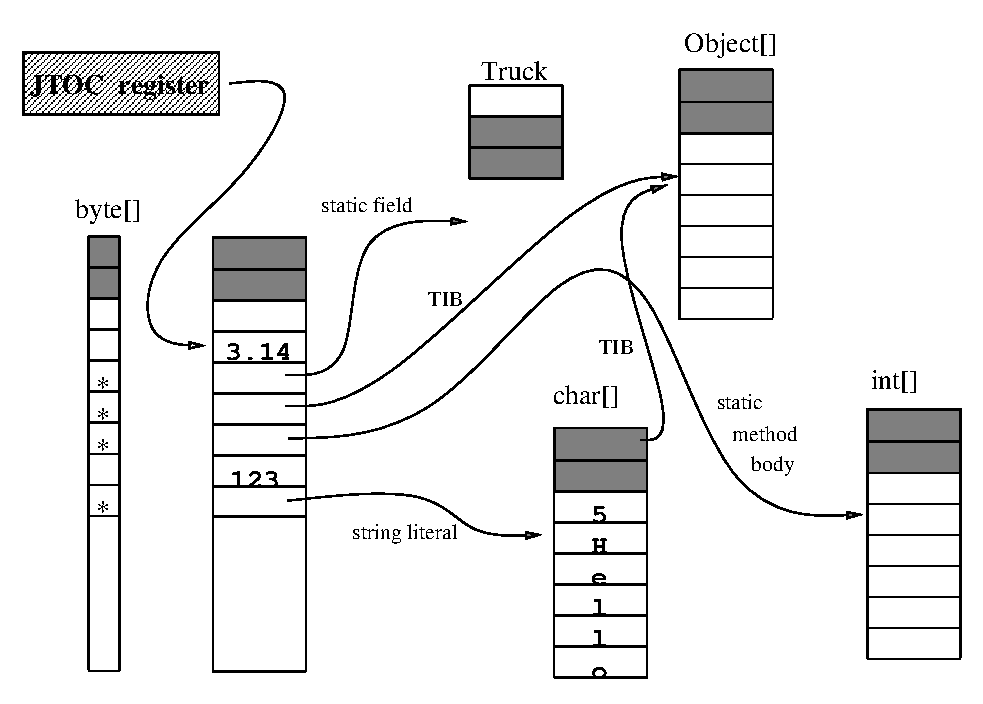
\psfig{file=jtoc.ps,height=3.5in}}
}\hfil
\end{gif}
\caption{The Jikes RVM Table Of Contents and other objects.}
\label{fig:jtoc}
\end{figure}
\index{literals}
\index{constants}
\index{dynamic type checking}
All of Jikes\trademark RVM's global data structures are stored in the JTOC. 
Literals, numeric
constants and references to String constants, are also stored there.
The JTOC also
contains references to the TIB for each class in the system.  
Since these 
structures can have many types and the JTOC is declared to be an array of 
{\tt int}s,  
Jikes RVM uses a descriptor array, co-indexed with the JTOC, 
to identify the entries containing references.
The JTOC
is depicted in figure~\ref{fig:jtoc}.  

\paragraph{Virtual Methods}
\index{virtual methods}
A TIB contains pointers to the compiled method 
bodies (executable code) for the virtual methods of its class. 
Thus, the TIB serves as Jikes RVM's virtual method table.
A virtual method dispatch entails loading the TIB pointer from 
the object reference, loading the address of the method
body at a given offset off the TIB pointer, and making an indirect
branch and link to it.

\paragraph{Static Fields and Methods} 
\index{static methods}
Static fields and methods are stored in the JTOC. Static method dispatch is 
simpler than virtual dispatch requiring only that the offset of method in the 
JTOC be read to find the address of the method. 

\paragraph{Lazy Method Compilation}
\index{lazy method compilation}
\index{deferred compilation}
\index{lazy method invocation stub}
The slots in the TIB or the JTOC may be filled in with 
a pointer to the compiled code for the method itself or if lazy method 
compilation is enabled and the method has not yet been compiled 
it may be filled in with
a pointer to the compiled code of the {\em lazy method invocation stub}.
If the lazy method invocation stub is invoked its action is to compile the 
method, substitute a pointer to the compiled code of the method in the slot in
the TIB or the JTOC from which it was invoked and then 
cause execution to jump to the start of the compiled method. 

\paragraph{Interface Methods}
\index{interface methods}
\index{IMT}
\index{conflict resolution stub}
Regardless of whether or not a method is overridden in a class that inherits it
virtual method dispatch is still very simple since the method body will be at
the same offset in the TIB in its defining class and in every class that 
inherits from it. 
However, where the method is an interface method, 
that is where it is invoked through an {\tt invoke\_interface} call rather than
an {\tt invoke\_virtual call}, its offset is not the same for every class that 
implements its interface and dispatch is more difficult.
The simplest, and least efficient way, of locating an interface method 
is to search all the virtual method entries in the TIB until a match is found.
Another way uses an {\em Interface Method Table} (IMT) which is much like the 
TIB. Any method that could be an interface method has a fixed offset into the 
IMT just as with the TIB. However, unlike in the TIB, two different methods may
share the same offset into the IMT. In this case, a {\em conflict resolution
stub} is inserted in the IMT. Conflict resolution stubs are
custom-generated machine code sequences that test the value of a
hidden parameter to dispatch to the desired interface method.
For more details, see
\xlink{{\tt VM\_InterfaceInvocation.java}}{\VMInterfaceInvocationURL}.

\JikesTMFooter

\subsection{VM Conventions}

%% footnotes not allowed in section headings, so we specialize
\htmlonly{\subsubsection{AIX\trademark VM Conventions}} 
\texonly{\subsubsection{AIX\trademark VM Conventions}} 
\label{aix-conventions}

\index{stack conventions}
\index{register conventions}
\index{calling conventions}

This section describes register, stack, and calling conventions that apply to 
Jikes RVM on PowerPC\PowerPCTMFootnote.

Stackframe layout and calling conventions may evolve as our understanding
of the Jikes RVM's performance improves.  Where possible API's should be used
to protect code against such changes.  In particular, we may move to
the AIX conventions at a later date.  Where code differs from the AIX
conventions, it should be marked with a comment to that effect containing
the string "AIX".

\noindent{\bf Register conventions}

Registers (general purpose, gp, and floating point, fp) can be roughly
categorized into four types:

\begin{description}
\item [Scratch]
     Needed for method prologue/epilogue.  Can be used by compiler between
     calls.

\item[Dedicated]
     Reserved registers with known contents:
\begin{description}
\item [JTOC - JikesRVM Table Of Contents]
        Globally accessible data: constants, static fields and methods.

\item [FP - Frame Pointer]
        Current stack frame (thread specific).

\item [TI - Thread (locking) Id]
        Used to set (and test) the locking field of light weight object
        locks.  Can also be shifted to get the index of an object
        representing the current thread in into a global array.

\item [PR - Processor register]
        An object representing the current virtual processor (the one
        executing on the CPU containing these registers).  A field in
        this object contains a reference to the object representing
        the VM\_Thread being executed.
\end{description}

\item [volatile ("caller save", or "parameter")]
     Like scratch registers these can be used by the compiler as
     temporaries, but they are not preserved across calls.  (Volatile
     registers differ from scratch registers in that volatiles
     can be used to pass parameters and result(s) to and from
     methods.)

\item [Nonvolatile ("callee save", or "preserved")]
     These can be used (and are preserved across calls), but they must be
     saved on method entry and restored at method exit.  Highest numbered
     registers are to be used first.  (At least initially, nonvolatile
     registers will not be used to pass parameters.)

\item[Condition Register's 4-bit fields]
\begin{description}
\item    [CR0 - CR1] scratch

\item    [CR2 - TSCR] dedicated (thread switching, bit 8 TSCRB) (this
     convention is being phased out, and in fact is not being used in RVM 2.0)

\item    [CR3 - CR7] scratch
\end{description}
\end{description}


\noindent{\bf Stack conventions}

Stacks grow from high memory to low memory.
The layout of the stackframe appears in a block comment in
\xlink{{\tt \$RVM\_ROOT/rvm/src/vm/arch/powerpc/VM\_StackframeLayoutConstants.java}}
{\PPCStackframeLayoutURL}.

\noindent{\bf Calling Conventions}

\begin{description}
\item[Parameters]

    All parameters (that fit) are passed in VOLATILE registers.  Object
    reference and int parameters (or results) consume one GP register; long
    parameters, two gp registers (low-order half in the first);  float and
    double parameters, one fp registers.  Parameters are 
    assigned to registers
    starting with the lowest volatile register through the highest volatile
    register to the highest nonvolatile of the required kind (gp or fp).

    Any additional parameters are passed on the stack in an parameter spill
    area of the caller's stack frame.  The first spilled parameter occupies
    the lowest memory slot.  Slots are filled in the order that parameters
    are spilled.

    An int, or object reference, result is returned in the first volatile
    gp register; a float or double result is returned in the first volatile
    fp register; a long result is returned in the first two volatile gp
    registers (low-order half in the first);

\item [Method prologue responsibilities] (some of these can be omitted for leaf
  methods):

\begin{enumerate}
\item Execute a stackoverflow check, and grow the thread stack if necessary.

\item Save the caller's next instruction pointer (callee's return address,
       from the Link Register).

\item Save any nonvolatile floating-point registers used by callee.

\item Save any nonvolatile general-purpose registers used by callee.

\item Store and update the frame pointer FP.

\item Store callee's compiled method ID 

\item Check to see if the Java\trademark thread must yield the VM\_Processor
(and yield if threadswitch was requested). 
\end{enumerate}

\item [Method epilogue responsibilities]

\begin{enumerate}
\item Restore FP to point to caller's stack frame.

\item Restore any nonvolatile general-purpose registers used by callee.

\item Restore any nonvolatile floating-point registers used by callee.

\item Branch to the return address in caller.
\end{enumerate}
\end{description}

\subsubsection{Linux/IA32 VM Conventions} \label{lintel-conventions}
\index{stack conventions}
\index{register conventions}
\index{calling conventions}

This section describes register, stack, and calling conventions that
apply to Jikes RVM on Linux/IA32.  {\em Linux/IA32 conventions are still
changing; be sure to check the relevant files for the most accurate
information!}

\noindent{\bf Register conventions}

\begin{description}
\item [EAX]
    First GPR parameter register, first GPR result value (high-order part
    of a long result), otherwise volatile (caller-save).

\item[ECX]
    Scratch.

\item[EDX]
    Second GPR parameter register, second GPR result value (low-order part
    of a long result), otherwise volatile (caller-save).

\item[EBX]
    Nonvolatile.

\item[ESP]
    Stack pointer.

\item[EBP]
    Nonvolatile.

\item[ESI]
    Processor register, reference to the VM\_Processor object for the current
    virtual processor.

\item[EDI]
    Nonvolatile.  (used to hold JTOC in baseline compiled code)

\end{description}

\noindent{\bf Stack conventions}

Stacks grow from high memory to low memory.
The layout of the stackframe appears in a block comment in
\xlink{{\tt
\$RVM\_ROOT/rvm/src/vm/arch/intel/VM\_StackframeLayoutConstants.java}}
{\LintelStackframeLayoutURL}.

\noindent{\bf Calling Conventions}

\begin{description}
\item[At the beginning of callee's prologue]
The first two areas of the callee's stackframe (see above) have been
     established.  ESP points to caller's return address.
     Parameters from caller to callee are as mandated by 
\xlink{{\tt
\$RVM\_ROOT/rvm/src/vm/arch/intel/VM\_RegisterConstants.java}}
{\LintelRegisterConstantsURL}.
\item[After callee's epilogue]
     Callee's stackframe has been removed.  ESP points to the word above where
     callee's frame was.  The framePointer field
     of the VM\_Processor object pointed to by ESI points to A's
     frame.  If B returns a floating-point result, this is at
     the top of the fp register stack.  If B returns a long, the
     low-order word is in EAX and the high-order word is in EDX.
     Otherwise, if B has a result, it is in EAX.

\end{description}

\JavaTMFooter

\AIXPPCTMFooter

\subsection{Class Loading} \label{sssec:classLoading}
\index{class loading}

Jikes\trademark RVM implements the Java\trademark programming
language's dynamic class 
loading. While a class is being loaded it 
can be in one of five states. These are
\begin{description}
\item[vacant] a forward reference exists to the class but loading has not yet 
begun.
\item[loaded] the class's bytecode file has been read and parsed successfully.
\item[resolved] the superclass of this class has been loaded and resolved and
the offsets (whether in the object itself, the JTOC, or the class's TIB) of its 
fields and methods have been calculated.
\item[instantiated] the superclass has been instantiated and pointers to the
compiled methods have been inserted into the JTOC(for static methods) and the
TIB (for virtual methods).
\item[initializing] the superclass has been initialized and the class
initializer is being run.
\item[initialized] the superclass has been initialized and the class
initializer has been run.
\end{description}

The class passes through these states in the following fashion.

\paragraph{Vacant}
The 
\xlink{{\tt VM\_Class}}{\VMClassURL} 
object for this class has been created and registered. 
A class can be in this state if a reference to the class exists in a constant
pool of some other class.

\paragraph{Loaded} 
\index{constant pool}
In this state the class file has been read and parsed.  The constant pool has 
been constructed. The declared methods and fields of the class have been loaded.
Loading a method or field consists of reading its modifiers and attributes.

\paragraph{Resolved}
In this state the superclass of this class has been loaded and resolved. 
A list of the virtual methods and instance fields of this class, including the 
methods and fields
inherited from its superclass has been constructed and the offsets for the 
instance fields have been calculated.  
Space has been allocated in the JTOC for all static fields of the class and for
static method pointers and the appropriate offsets calculated.
The TIB has been initialized and offsets for the virtual methods have been
calculated.

\paragraph{Instantiated}
In this state the superclass of this state has been instantiated. 
The slots in the TIB are filled in with pointers to the compiled code for the 
virtual methods. 
The slots in the JTOC are filled in with pointers to the compiled code for the 
static methods.

\paragraph{Initializing} 
\index{class initializer}
In this state the superclass has been initialized. The class
initializer is being run. 

\paragraph{Initialized} 
\index{class initializer}
In this state the superclass has been initialized. The class initializer has 
been run. 

\JavaTMFooter

\JikesTMFooter

\subsection{Thread System}\label{sec:threads}

This section provides some explanation of how Java\TMweb{} threads are
scheduled and synchronized by Jikes\TMweb{} RVM.\@

\index{threads}
\index{scheduling}
\index{locking}

\label{threads:single-virtual-processor}All Java threads (application threads, garbage collector threads, {\em
etc.})  derive from 
\xlink{{\tt VM\_Thread}}{\VMThreadURL}.  
These threads are multiplexed onto
one or more virtual processors (see 
\xlink{{\tt VM\_Processor}}{\VMProcessorURL}).  Normally, the
number of Jikes RVM virtual processors to use is a command line argument
({\it e.g.}\ {\tt -X:processors=4}) Generally, there should be one Jikes RVM
virtual processor for each CPU on an SMP.\@  Additional virtual
processors may be created to handle threads executing non-Java code
through the Java JNI.\@  Multiple virtual processors require a working
pThread library, each virtual processor being bound to a pThread.  It
is possible to build a system that only uses one virtual processor by
setting the preprocessor directive 
\varName{RVM\_\-FOR\_\-SIN\-GLE\_\-VIR\-TU\-AL\_\-PRO\-CES\-SOR} to 1.  This may give a minor
performance benefit on uniprocessors. See the configuration file
{\tt BaseBaseCopyMSUP} for examples of
using this preprocessor directive.

Threads that are not executing are either placed on thead queues
(deriving from 
\xlink{\texttt{VM\_\-Ab\-stract\-Thread\-Queue}}{\VMAbstractThreadQueueURL}
) or are proxied (see below).
Thread queues are either global or (virtual) processor local.  The
latter do not require synchronized access but global queues do.
Unfortunately, we did not see how to use Java monitors to provide
this synchronization.  (In part, because it is needed to implement
monitors, see below.)  Instead this low-level synchronization is
provided by 
\xlink{{\tt VM\_\-Pro\-ces\-sor\-Lock}}{\VMProcessorLockURL}s.

Transferring execution from one thread (A) to another (B) is a complex
operation negotiated by the {\tt yield} and {\tt morph} methods of
VM\_Thread and the {\tt dispatch} method of VM\_Processor.  {\tt
yield} places A on an indicated queue (releasing the lock on the
queue, if it is global).  {\tt morph} does some additional
housekeeping and transfers control to {\tt dispatch} which selects the
next thread to execute. Dispatch then invokes {\tt
VM\_Ma\-gic.thread\-Switch} to save the hardware context of A and restore
the hardware context of B.\@  It now appears as if B's previous call to
{\tt dispatch} has just returned and it continues executing. While
dispatching is proceeding (from the time A is enqueued until B's
hardware context is restored), the {\tt be\-ing\-Dis\-patched} field of A is
set to prevent it from being scheduled for execution on some other
virtual processor while it is still executing in {\tt morph } or {\tt
dispatch}. 

Beginning with version 2.0.1, Jikes RVM has a simple load balancing
mechanism. Every once in a while, a thread will move from one virtual
processor to the next.  Such movement happens when a thread is
interrupted by a timer tick (or garbage collection) or when it comes
off a global queue (such as, the queues waiting for a heavy-weight
lock, see \xlink{{\tt VM\_Lock}}{\VMLockURL}).  Such migration will be
inhibited if the thread is the last (non-idle) executable thread on
its current virtual processor.  

If a virtual processor has no other executable thread, its idle thread
runs.  This thread posts a request for work and then busy-waits for a
short time (currently 0.001 seconds).  If no work arrives in that
period, the virtual processor surrenders the rest of its time slice
back to the operating system.  If another virtual processor notices
that this one needs work, it will tranfer an extra runnable thread (if
it has one) to this processor.  When work arrives, the idle thread
yields to an idle queue, and the recently transferred thread begins
execution.

Currently, Jikes RVM has no priority mechanism, that is, all threads run at
the same priority.

If Jikes RVM detects that a thread is stuck executing native code (JNI)
for a long time, it temporarily prevents it from returning to Java code and
creates a new pThread (or recycles one previously created for this 
purpose) and transfers the stuck thread's virtual processor to the
new pThread.  When the stuck thread returns to Java code, the pThread
executing it is deactivated and added to a pool of available pThreads.
Currently, this mechanism does not work on Linux and is disabled there.

Jikes RVM uses a light-weight locking scheme to implement Java monitors (see
\xlink{{\tt VM\_Lock}}{\VMLockURL} and 
\xlink{{\tt VM\_\-Thin\-Lock}}{\VMThinLockURL}). The exact details of the
locking scheme are dependent on which variant of 
\xlink{{\tt VM\_\-Ja\-va\-Hea\-der.java}}{\VMJavaHeaderURL} is selected at
system build time.  If an object instance has a light weight lock,
then some bits in the object header are used for locking.  
If the top bit is set, the remainder of the bits 
are an index into an array of heavy-weight locks.
Otherwise, if the object is locked, these bits contain the id of the
thread that holds the lock and a count of how many times it is held.
If a thread tries to lock an object locked with a light-weight lock by
another thread, it can spin, yield, or inflate the lock.  Spinning is
probably a bad idea.  The number of times to yield before inflating is
a matter open for investigation (as are a number of locking
issues, see {\tt VM\_Lock}).  Heavy-weight locks contain an {\tt
enteringQueue} for threads trying to acquire the lock.

A similar mechanism is used to implement Java wait/notification
semantics.  Heavy-weight locks contain a {\tt waitingQueue} for
threads blocked at a Java {\tt wait}.  When a {\tt notify} is
received, a thread is taken from this queue and transferred to a ready
queue.  Priority {\tt wakeupQueue}s are used to implement Java sleep
semantics.  Logically, Java timed-wait semantics entail placing a
thread on both a {\tt waitingQueue} and a {\tt wakeupQueue}.  However, our
implementation only allows a thread to be on one thread queue at
a time.  To accommodate timed-waits, both {\tt wai\-ting\-Queue}s and
{\tt wake\-up\-Queue}s are queues of {\em proxies} rather than threads.
A \xlink{{\tt VM\_Proxy}}{\VMProxyURL} can represent the same thread
on more than one proxy queue.


\subsection{VM Callbacks}\label{sssec:callbacks}

\index{callbacks}

Jikes\TMweb{} RVM provides callbacks for many runtime events of
interest to the Jikes RVM 
programmer, such as classloading, VM boot image creation, and VM exit.  The
callbacks allow arbitrary code to be executed on any of the supported events.

The callbacks are accessed through the nested interfaces defined in the 
\xlink{{\tt VM\_\-Call\-backs}}{\VMCallbacksURL} 
class.  There is one interface per event type.  To be notified
of an event, register an instance of a class that implements the corresponding
interface with {\tt VM\_Callbacks} by calling the corresponding {\tt add...()}
method.  For example, to be notified \link{when a class is instantiated}[ (see section~\Ref)]{sssec:classLoading}, first implement the {\tt
VM\_Callbacks.ClassInstantiatedMonitor} interface, and then call {\tt
VM\_\-Call\-backs.add\-Class\-In\-stan\-ti\-a\-ted\-Mon\-i\-tor()} with an instance of your class.
When any class is instantiated, the {\tt notifyClassInstantiated} method in
your instance will be invoked.

\xlink{Jikes RVM supports callbacks for a number of events}[; see 
{\tt VM\_Callbacks} for the list of currently
supported callbacks]{\VMCallbacksURL}.

The appropriate interface names can be obtained by appending ``Monitor'' to the
event names (e.g. the interface to implement for the {\tt MethodOverride} event
is {\tt VM\_\-Call\-backs.Me\-thod\-Ov\-er\-ride\-Mo\-ni\-tor}).  Likewise, the method to
register the callback is ``add'', followed by the name of the interface (e.g.
the register method for the above interface is {\tt
VM\_\-Call\-backs.add\-Me\-thod\-O\-ver\-ride\-Mon\-i\-tor()}).

Since the events for which callbacks are available are internal to the VM,
there are naturally some limitations on the behavior of the callback code.  For
example, as soon as the exit callback is invoked, all threads are considered
daemon threads (i.e. the VM will not wait for any new threads created in the
callbacks to complete before exiting).  Thus, if the exit callback creates any
threads, it has to {\tt join()} with them before returning.  These limitations
may also produce some unexpected behavior.  For example, while there is an
elementary safeguard on any classloading callback that prevents recursive
invocation (i.e. if the callback code itself causes classloading), there is no
such safeguard across events, so, if there are callbacks registered for both
{\tt ClassLoaded} and {\tt Class\-In\-stan\-ti\-a\-ted} events, and the {\tt
Class\-In\-stan\-ti\-a\-ted} callback code causes dynamic class loading, the {\tt
ClassLoaded} callback will be invoked for the new class, but not the {\tt
Class\-In\-stan\-ti\-a\-ted} callback.

Examples of callback use can be seen in the {\tt VM\_Controller} class in the
adaptive system and the {\tt VM\_GCStatistics} class.

\subsubsection{An Example: Modifying SPECjvm98 to Report the End of a
                  Run}\label{sssec:callback-example}

The SPECjvm\Rboth{}98 benchmark suite is configured to run one or more
benchmarks 
a particular number of times.  For example, the following runs the
{\tt compress} benchmark for 5 iterations:
\begin{example}
 rvm SpecApplication -m5 -M5 -s100 -a \_201\_compress
\end{example}
It is sometimes useful to have the VM notified when the application
has completed an iteration of the benchmark.   This can be performed
by using the {\tt VM\_Callbacks} interface.  The specifics are
specified below:
\begin{enumerate}
\item Modify {\tt spec/harness/ProgramRunner.java} as follows:
	\begin{enumerate}

	\item add an import statement for the {\tt VM\_Callbacks} class:
        \begin{example}
        import com.ibm.JikesRVM.VM\_Callbacks;
        \end{example}

	\item before the call to {\tt runOnce} add the following:
        \begin{example}
        VM\_Callbacks.notifyAppRunStart(run);
        \end{example}

	\item after the call to {\tt runOnce} add the following:
        \begin{example}
        VM\_Callbacks.notifyAppRunComplete(run);
        \end{example}

	\end{enumerate}

\item Recompile the modified file using {\tt javac} or {\tt jikes}:
\begin{example}
javac -classpath 
   .:\$RVM\_\-BUILD/\-RVM.clas\-ses:\$RVM\_\-BUILD/\-RVM.clas\-ses/\-rvmrt.jar
   spec/\-har\-ness/\-Pro\-gram\-Run\-ner.java
\end{example}
or
\begin{example}
jbuild.tool spec/\-har\-ness/\-Pro\-gram\-Run\-ner.java
\end{example}

\item Run Jikes RVM as you normally would using the SPECjvm98 benchmarks.
\end{enumerate}

In the current system the {\tt VM\_Controller} class will gain control
when these callbacks are made and print a message into the AOS log
file (called AOSLog.txt, by default).



\subsection{Support for Soot-style Annotations}\label{sssec:annotations}
Jikes RVM optionally supports reading and using Soot-style class file
annotations.  Such annotations can specify that a null check or bounds
check is redundant for a particular byte code instruction.  These
annotations are produced by the {\bf Soot} class file optimizer
available from
\xlink{\SOOTURL}{\SOOTURL}.  

When the annotations command-line option is true, class file
annotations are processed by \xlink{{\tt
VM\_Method.java}}{\VMMethodURL} and stored internally in Jikes RVM.
During compilation (either baseline or optimizing), the compiler 
queries the {\tt VM\_Method} class for a particular bytecode to
determine if the generation of a null or bounds check can be
surpressed. 

Processing Soot-style annotations is not enabled, by default.  To
enable this support specify {\tt ``annotations=true''} to the
appropriate compiler.  For example, use {\tt -X:irc:annotations=true}
for non-adaptive images and {\tt -X:aos:irc:annotations=true} for
adaptive images.





\T \newpage
\section{Optimizing Compiler Implementation Details}
\label{section:optdetails}
This section provides some information on various
implementation details for the Jikes\trademark RVM optimizing compiler.

%%%%%%%%%%%%%%%%%%%%
\subsection{Options}
\label{section:optdetails:options}

\index{command-line options}
\index{OPT\_Options class}
The Jikes RVM stores command-line options to the optimizing compiler 
as fields in an object of type {\tt OPT\_Options}.
The Jikes RVM build process generates the {\tt OPT\_Options.java} 
file automatically from a template.  

\index{BooleanOptions.dat}
\index{ValueOptions.dat}
To add or modify the command-line options in {\tt OPT\_Options.java},
you must modify either {\tt BooleanOptions.dat} or 
{\tt ValueOptions.dat}.  You should describe your desired
command-line option in a format described below.
Your option will be generated the next time you build the
system.

%%%%%%%%%%%%%%%%%%%%%%%%%%%%%%%%%%
\subsubsection{BooleanOptions.dat}
\index{BooleanOptions.dat}

The {\tt BooleanOptions.dat} file defines boolean options for
the optimizing compiler.  The file describes each command-line option 
by a two-line record, and each record is separated
by a blank line.  Long lines can be continued using ``$\backslash$''.
{\bf NOTE:} blank lines {\em are} important!
Lines starting with ``\#'' are ignored.

The first line must have the following format
\begin{quote}
\begin{verbatim}
FULL_NAME OPT_LEVEL DEFAULT_VALUE {SHORT_NAME}
\end{verbatim}
\end{quote}
where
\begin{itemize}
\item {\tt FULL\_NAME} gives the name of the boolean field in {\tt OPT\_Options.java}
\item {\tt OPT\_LEVEL} gives the minimum optimization level that automatically sets this field true
\item {\tt DEFAULT\_VALUE} of {\tt true} or {\tt false}
\item {\tt SHORT\_NAME} is an optional field which defines a mnemonic by which the command-line processor recognizes this option.
\end{itemize}

The second line of each record must hold a short textual description of
the semantics of the option. 
The system will print this description 
when so instructed 
by the command-line option {\tt -X:irc:help} (see Appendix~\ref{appendix:nonadaptive:cmdline}).

For example, the two line record in {\tt BooleanOptions.dat}
that defines the option of whether
to perform local scalar replacement is
\begin{verbatim}
LOCAL_SCALAR_REPLACEMENT 1 true local_sr
Perform local scalar replacement
\end{verbatim}

%%%%%%%%%%%%%%%%%%%%%%%%%%%%%%%%
\subsubsection{ValueOptions.dat}
\index{ValueOptions.dat}

The {\tt ValueOptions.dat} file defines non-boolean options for
the optimizing compiler.  The file describes each command-line option 
with a three-line record, and each record is separated
by a blank line.  As with {\tt BooleanOptions.dat},
long lines can be continued using ``$\backslash$'' and
blank lines are once again significant.
Lines starting with ``\#'' are ignored.

The first line must have the following format
\begin{quote}
\begin{verbatim}
TAG FULL_NAME TYPE DEFAULT_VALUE {SHORT_NAME}
\end{verbatim}
\end{quote}
where
\begin{itemize}
\item {\tt TAG} is 'E' for an Enumeration type, and 'V' for a value type.  Further instructions for Enumeration types appear below.
\item {\tt FULL\_NAME} gives the name of the field in {\tt OPT\_Options.java}
\item {\tt TYPE} is one of 'byte', 'int', or 'String', and gives the primitive datatype for the value in OPT\_Options.java
\item {\tt DEFAULT\_VALUE} is the default value for the option
\item {\tt SHORT\_NAME} is an optional field which defines a mnemonic by which the command-line processor recognizes this option.
\end{itemize}

The second line of each record must hold a short textual description of
the semantics of the option.  
The system will print this description 
when so instructed 
by the command-line option {\tt -X:irc:help} (see Section~\ref{appendix:nonadaptive:cmdline}).

The third line of each record is used for enumeration options, and must
be left blank for non-enumeration options.

For example, the three-line record in {\tt ValueOptions.dat}
that defines the maximum inlining depth when using static inlining
heuristics is
\begin{verbatim}
V IC_MAX_INLINE_DEPTH int 5
Static inlining heuristic: Upper bound on depth of inlining
<blank line>
\end{verbatim}

Enumeration options provide a mechanism to define an option in terms of 
a small fixed set of choices.  For an enumeration option, the third line
of the record must contain a specification for each value that the
enumeration can take.  Each such specification must have the following
format:
\begin{verbatim}
"ITEM_NAME QUERY_NAME CMD_NAME"
\end{verbatim}
where
\begin{itemize}
\item {\tt ITEM\_NAME} gives the name of the enumeration value in {\tt OPT\_Options.java}
\item {\tt QUERY\_NAME} gives the name of an accessor function which returns {\tt true} iff the enumeration takes the value {\tt ITEM\_NAME}.
\item {\tt CMD\_NAME} is the name to pass on the command-line to set the enumeration to this value.
\end{itemize}
The quotes are important, and the specifications should be
space-separated.

For example, Jikes RVM supports a choice of three options for floating-point
optimization rules.  The three-line record describing these options is:
\begin{verbatim}
E FP_MODE byte FP_STRICT
Selection of strictness level for floating point computations
"FP_STRICT strictFP strict" \
"FP_ALLOW_FMA allowFMA allow_fma" \
"FP_LOOSE allowAssocFP allow_assoc"
\end{verbatim}
Notice how the third line was broken up by using ``$\backslash$''.

So, by default, Jikes RVM uses the {\em strict} floating-point
semantics.  To use 
the option that allows fused multiply-add instructions, 
specify {\tt -X:irc:allow\_fma} on the command-line.
Given an {\tt OPT\_Options} object called {\tt options}, your code can
query if fma is allowed by testing {\tt options.allowFMA()}.

%%%%%%%%%%%%%%%%%%%%%%%%%%%%%%%
\subsection{Method Compilation}
\label{sec:optdriver}
\index{compilation}
\index{optimizations}
\index{IR}
\index{HIR}
\index{LIR}
\index{MIR}
The fundamental unit for optimization in the Jikes RVM is a single method. 
The optimization of a method consists of a series of 
compiler phases performed on the method. These 
phases transform the  
IR (intermediate representation) from bytecodes through 
HIR (high-level intermediate representation), 
LIR (low-level intermediate representation), and 
MIR (machine intermediate representation) and finally into machine code. 
Various optimizing transformations are performed at each level of IR.

\index{OPT\_CompilationPlan class}
\index{VM\_Method class}
\index{OPT\_OptimizationPlanElement class}
An object of the class 
\xlink{{\tt OPT\_CompilationPlan}}{\OPTCompilationPlanURL} 
contains all the  
information necessary to generate machine code for a method. 
An instance of this class includes, among other fields, 
the 
\xlink{{\tt VM\_Method}}{\VMMethodURL} 
to be compiled and the array of 
\xlink{{\tt OPT\_OptimizationPlanElements}}{\OPTOptimizationPlanElementURL} 
which define the compilation steps.
The {\tt execute} method of an
\xlink{{\tt OPT\_CompilationPlan}}{\OPTCompilationPlanURL} 
invokes the optimizing compiler to generate machine code for the method,
executing the compiler phases as listed in the plan's
{\tt OPT\_OptimizationPlanElement}s.

\index{OPT\_OptimizationPlanner class}
The 
\xlink{{\tt OPT\_OptimizationPlanner}}{\OPTOptimizationPlannerURL} 
class defines the standard phases used in a compilation.
This class
contains a static field, called {\tt masterPlan}, which contains all
possible {\tt OPT\_OptimizationPlanElement}s.
The structure of the master plan is 
a tree. Any element may either be an atomic element (a leaf of the 
tree), or an aggregate element (an internal node of the tree).
The master plan has the following general structure:

\begin{itemize}
\item elements which convert bytecodes to HIR
\item elements which perform optimization transformations on the HIR
   \begin{itemize}
   \item elements which perform optimization transformations using SSA form
   \end{itemize}
\item elements which convert HIR to LIR
\item elements which perform optimization transformations on the LIR
   \begin{itemize}
   \item elements which perform optimization transformations using SSA form
   \end{itemize}
\item elements which convert LIR to MIR
\item elements which perform optimization transformations on MIR 
\item elements which convert MIR to machine code
\end{itemize}


\index{optimization plan}
A client (compiler driver) constructs a specific optimization plan by including all the 
{\tt OPT\_OptimizationPlanElement}s contained in the master plan which are 
appropriate for this compilation instance. 
Whether or not an element should be part of a compilation plan is determined 
by its {\tt shouldPerform} method. For each atomic element, the values in the
{\tt OPT\_Options} object are generally used to determine whether the element
should be included in the compilation plan. Each aggregate element must be 
included when any of its component elements must be included. 

Each element must have a {\tt perform} method defined which takes the IR as
a parameter. It is expected, but not required, that the {\tt perform}
method will modify the IR. 
The perform method of an aggregate element will invoke the 
perform methods of its elements.

\index{OPT\_CompilerPhase class}
Each atomic element is an object of the final class 
{\tt OPT\_OptimizationPlanAtomicElement}. The main work of this class
is performed by its {\em phase}, an object of type 
\xlink{{\tt OPT\_CompilerPhase}}{\OPTCompilerPhaseURL}. The
{\tt OPT\_CompilerPhase} class is not final; each phase overrides this class,
in particular it overrides the {\tt perform} method, which is invoked by its 
enclosing element's {\tt perform} method. All the state associated with 
the element
is contained in the {\tt OPT\_CompilerPhase}; no
state is in the element.

Every optimization plan consists of a selection of elements from the master 
plan;
thus two optimization plans associated with different methods 
will share the same component element objects. 
Clearly, it is undesirable to share state 
associated with a particular compilation phase between two
different method compilations. In order to prevent this, the {\tt perform}
method of an atomic element creates a new instance of its phase immediately 
before calling the phase's {\tt perform} method. 
In the case where the phase
contains no state the {\tt newExecution} method of 
{\tt OPT\_CompilerPhase} can be overridden to return the phase itself rather 
than a clone of the phase~\footnote{Since this coding pattern may result
in unintended memory leaks, overriding {\tt newExecution} may be
disallowed in future releases.}.


%%%%%%%%%%%%%%%%%%%%%%%%%
\subsection{IR Operators}
\index{IR}
\index{instructions}
\index{operators}

The optimizing compiler intermediate representation (IR) includes a list
of instructions.  Each instruction includes an operator and zero or
more operands.

\index{OPT\_Operators class}
\index{OperatorList.dat}
The IR operators are defined by the class {\tt OPT\_Operators}, which in
turn is automatically generated from a template by a driver.  The input to the
driver are two files, both called {\tt OperatorList.dat}.  One input
file resides in {\tt \$RVM\_ROOT/rvm/src/vm/compilers/optimizing/ir/instruction} and defines machine-independent
operators.  The other resides in {\tt \$RVM\_ROOT/rvm/src/vm/arch/\{arch\}/compilers/optimizing/ir/instruction}
and defines machine-dependent operators, where \{arch\} is the
specific architecture of interest, such as PowerPC\PowerPCTMFootnote.

Each operator in {\tt OperatorList.dat} is defined by a five-line record,
consisting of:
\begin{itemize}
\item {\tt SYMBOL}: a static symbol to identify the operator
\item {\tt INSTRUCTION\_FORMAT}: the instruction format class that accepts this operator.  See Section~\ref{iformats} for more information.
\item {\tt TRAITS}: a set of characteristics of the operator, composed with a bit-wise or ($|$) operator.  See {\tt OPT\_Operator.java} for a list of valid traits.
\item {\tt IMPLDEFS}: set of registers implicitly defined by this operator; usually applies only to machine-dependent operators
\item {\tt IMPLUSES}: set of registers implicitly used by this operator; usually applies only to machine-dependent operators
\end{itemize}

For example, the entry in {\tt OperatorList.dat} that defines the integer
addition operator is
\begin{verbatim}
INT_ADD
Binary
none
<blank line>
<blank line>
\end{verbatim}

The operator for a conditional branch based on values of two references is
defined by
\begin{verbatim}
REF_IFCOMP
IntIfCmp
branch | conditional
<blank line>
<blank line>
\end{verbatim}

Additionally,  the machine-specific {\tt OperatorList.dat} file contains 
another line of information for use by the assembler.  See the file
for details. 

\PowerPCTMFooter

%%%%%%%%%%%%%%%%%%%%%%%%%%%%%%%%
\subsection{Instruction Formats}\label{iformats}
\index{instructions}
\index{instructionFormats.java}

Every IR instruction fits one of the pre-defined {\em Instruction Formats}.
The Java package {\tt instructionFormats} defines roughly 75 architecture-independent
instruction formats.  For each instruction format, the package includes a class
that defines a set of static methods by which optimizing compiler
code can access an instruction of that format.

For example, {\tt INT\_MOVE} instructions conform to the {\tt Move}
instruction format.  The following code fragment shows code that uses the
{\tt OPT\_Operators} interface and the {\tt Move} instruction format:
\begin{verbatim}
import instructionFormats.*;
class X {
  void foo(OPT_Instruction s) {
    if (Move.conforms(s)) {     // if this instruction fits the Move format
      OPT_RegisterOperand r1 = Move.getResult(s);
      OPT_Operand r2 = Move.getVal(s);
      System.out.println("Found a move instruction: " + r1 + " := " + r2);
    } else {
      System.out.println(s + " is not a MOVE");
    }
  }
}
\end{verbatim}

This example shows just a subset of the access functions defined for the
Move format.  Other static access functions can set each operand 
(in this case, {\tt Result} and {\tt Val}), query each operand for
nullness, clear operands, create Move instructions, mutate other
instructions into Move instructions, and check the index of a particular
operand field in the instruction.  See the javadoc reference for a complete
description of the API.

\index{InstructionFormatList.dat}
Each fixed-length instruction format is defined in the text file 
{\tt \$RVM\_ROOT/rvm/src/vm/compilers/optimizing/ir/instruction/InstructionFormatList.dat}.
Each record in this file has four lines:
\begin{itemize}
\item {\tt NAME}: the name of the instruction format
\item {\tt SIZES}: the number of operands defined, defined and used, and used 
\item {\tt SIG}: a description of each operand, each description given
by
\begin{itemize}
\item {\tt D/DU/U}: Is this operand a def, use, or both?
\item {\tt NAME}: the unique name to identify the operand
\item {\tt TYPE}: the type of the operand (a subclass of {\tt OPT\_Operand}
\item {\tt [opt]}: is this operand optional?
\end{itemize}
\item {\tt VARSIG}: a description of repeating operands, used for
variable-length instructions.
\end{itemize}

So for example, the record that defines the {\tt Move} instruction format
is
\begin{verbatim}
Move
1 0 1
"D Result OPT_RegisterOperand" "U Val OPT_Operand"
<blank line>
\end{verbatim}

This specifies that the {\tt Move} format has two operands, one def and one
use.  The def is called {\tt Result} and must be of
type {\tt OPT\_RegisterOperand}.
The use is called {\tt Val} and must be of type {\tt OPT\_Operand}.

A few instruction formats have variable number of operands.  The
format for these records is given at the top of {\tt InstructionFormatList.dat}.
For example, the record for the variable-length {\tt Call} instruction
format is: 
\begin{verbatim}
Call
1 0 3 1 U 4
"D Result OPT_RegisterOperand" \
"U Address OPT_Operand" "U Method OPT_MethodOperand" "U Guard OPT_Operand opt"
"Param OPT_Operand"
\end{verbatim}
This record defines the {\tt Call} instruction format.  The second line
indicates that this format always has at least 4 operands (1 def and 3 uses),
plus a variable number of uses of one other type.  The trailing
4 on line 2 tells the template generator to generate special constructors
for cases of having 1, 2, 3, or 4 of the extra operands.
Finally, the record names the {\tt Call} instruction operands and
constrains the types.  The final line specifies the name and
types of the variable-numbered operands.  In this case, a {\tt Call}
instruction has a variable number of (use) operands called {\tt Param}.
Client code can access the {\tt i}th parameter operand of a {\tt Call}
instruction {\tt s} by calling {\tt Call.getParam(s,i)}.

A number of instruction formats share operands of 
the same semantic meaning and name.  For convenience in accessing
like instruction formats, the template generator supports four
common operand access types:
\begin{itemize}
\item {\tt ResultCarrier}: provides access to an operand of type {\tt OPT\_RegisterOperand} named {\tt Result}.
\item {\tt GuardResultCarrier}: provides access to an operand of type {\tt OPT\_RegisterOperand} named {\tt GuardResult}.
\item {\tt LocationCarrier}: provides access to an operand of type {\tt OPT\_LocationOperand} named {\tt Location}.
\item {\tt GuardCarrier}: provides access to an operand of type {\tt OPT\_Operand} named {\tt Guard}.
\end{itemize}

For example, for any instruction {\tt s} that carries a {\tt Result} operand
(eg. {\tt Move}, {\tt Binary}, and {\tt Unary} formats), client code can call
{\tt ResultCarrier.conforms(s)} and {\tt ResultCarrier.getResult(s)} to access
the {\tt Result} operand.

Finally, a note on rationale.  Religious object-oriented philosophers
will cringe at the InstructionFormats.  Instead, all this
functionality could be implemented more cleanly with a hierarchy of
instruction types exploiting (multiple) inheritance.  We rejected the
class hierarchy approach due to efficiency concerns of frequent
virtual/interface method dispatch and type checks.  Recent
improvements in our interface invocation sequence and dynamic type
checking algorithms may alleviate some of this concern.

%%%%%%%%%%%%%%%%%%%%%%%
\subsection{BURS Rules}\label{burs}
\index{BURS}
\index{instruction selection}

The optimizing compiler uses the Bottom-Up Rewrite System (BURS) for
instruction selection.  BURS is essentially a tree pattern matching
system derived from Iburg by David R.\ Hanson.   (See ``Engineering a
Simple, Efficient Code-Generator Generator'' by Fraser, Hanson, and
Proebsting, LOPLAS 1(3), Sept.\ 1992.)
The instruction selection rules for each architecture are specified in an
architecture-specific file called {\tt LIR2MIR.rules}, which resides in
{\tt \$RVM\_ROOT/rvm/src/vm/arch/\{arch\}/compilers/optimizing/ir/conversions/lir2mir}, where \{arch\} is the
specific architecture of interest, such as PowerPC\PowerPCTMFootnote.
The rules are 
used in generating a parser, which transforms the IR.

Each rule in {\tt LIR2MIR.rules} is defined by a four-line record,
consisting of:
\begin{itemize}
\item {\tt PRODUCTION}: the tree pattern to be matched.  The format of each
pattern is explained below.
\item {\tt COST}: the cost of matching the pattern as opposed to skipping
it.  It is a Java\trademark expression that evaluates to an integer.
\item {\tt FLAGS}: specifies whether the rule actually represents a sequence
of instructions (EMIT\_INSTRUCTION) or a transformation of operands
(NOFLAGS). Other flags can be used to control the order of code
generation of a node's children.
\item {\tt TEMPLATE}: Java code to emit
\end{itemize}

Each production has a {\em non-terminal}, which denotes a value, followed
by a colon (``:''), followed by a dependence tree that produces that value.
For example, the rule resulting in memory add on the INTEL architecture is
expressed in the following way:
\begin{verbatim}
stm:    INT_STORE(INT_ADD_ACC(INT_LOAD(r,riv),riv),OTHER_OPERAND(r, riv))
ADDRESS_EQUAL(P(p), PLL(p), 17)
EMIT_INSTRUCTION
EMIT(MIR_BinaryAcc.mutate(P(p), IA32_ADD, MO_S(P(p), DW), \
                          BinaryAcc.getValue(PL(p))));
\end{verbatim}
The production in this rule represents the following tree:
\begin{verbatim}
         r     riv
          \    /
         INT_LOAD  riv
             \     /
           INT_ADD_ACC  r  riv
                    \   |  /
                   INT_STORE
\end{verbatim}
where {\tt r} is a non-terminal that represents a register or a tree
producing a register, {\tt riv} is a non-terminal that represents a register
(or a tree producing one) or an immediate value, and {\tt INT\_LOAD},
{\tt INT\_ADD\_ACC} and {\tt INT\_STORE} are operators ({\em terminals}).
{\tt OTHER\_OPERAND} is just an abstraction to make the tree binary.

There are multiple helper functions that can be used in Java code (both cost
expressions and generation templates).  In all code sequences the name
{\tt p} is reserved for the current tree node.  Some of the helper methods
are shortcuts for accessing properties of tree nodes:
\begin{itemize}
\item {\tt P(p)} is used to access the instruction associated with the
current (root) node,
\item {\tt PL(p)} is used to access the instruction associated with the left
child of the current (root) node (provided it exists),
\item {\tt PR(p)} is used to access the instruction associated with the
right child of the current (root) node (provided it exists),
\item similarly, {\tt PLL(p)}, {\tt PLR(p)}, {\tt PRL(p)} and {\tt PRR(p)}
are used to access the instruction associated with the
left child of the left child, right child of the left child, left child of
the right child and right child of the right child, respectively, of the
current (root) node (provided they exist).
\end{itemize}

What the above rule basically reads is the following:\\
If a tree shown above is seen, evaluate the cost expression (which, in this
case, calls a helper function to test whether the addresses in the
{\tt STORE} ({\tt P(p)}) and the {\tt LOAD} ({\tt PLL(p)}) instructions are
equal.  The function returns 17 if they are, and a special value
{\tt INFINITE} if not), and if the cost is acceptable, emit the {\tt STORE}
instruction ({\tt P(p)}) mutated in place into a machine-dependent
add-accumulate instruction ({\tt IA32\_ADD}) that adds a given value to the
contents of a given memory location.

The rules file is used to generate a file called {\tt ir.brg}, which, in
turn, is used to produce a file called {\tt OPT\_BURS\_STATE.java}.

For more information on helper functions look at
{\tt \$RVM\_ROOT/rvm/src/vm/arch/\{arch\}/compilers/optimizing/ir/conversions/lir2mir/OPT\_BURS\_Helpers.java}.
For more information on the BURS algorithm see
{\tt \$RVM\_ROOT/rvm/src/vm/compilers/optimizing/ir/conversions/lir2mir/OPT\_BURS.java}.

\JavaTMFooter

\PowerPCTMFooter


\subsection{OptTestHarness}\label{opttestharness}

For optimizing compiler development, it is sometimes useful to exercise
careful control over which classes are compiled, and with which
optimization level.  In many cases, a {\tt BaseOptSemiSpace} image will
suit this process.  This configuration invokes the optimizing compiler on
each method run.  Since the optimizing compiler is not in the boot image, 
you can modify its classes without re-linking the boot image.  Instead,
{\tt jbuild -nolink} will recompile the source files you edit, without
invoking the time-consuming boot image writing step.

The {\tt OptTestHarness} program provides even more control over the
optimizing compiler.  This driver program allows you to invoke the
optimizing compiler as an ``application'' running on top of the VM.
The most useful configuration for this is probably {\tt
BaseBaseOTHSemiSpace}; this image provides a BaseBase configuration with just
enough support to invoke the optimizing compiler through {\tt
OptTestHarness}.  Like the {\tt BaseOpt} images, you can use {\tt jbuild
-nolink} to skip a time-consuming boot image writing during development.

To use the {\tt OptTestHarness} program:
\begin{verbatim}
% rvm OptTestHarness -class Foo
\end{verbatim}
will invoke the optimizing compiler on all methods of class {\tt Foo.}

\begin{verbatim}
% rvm OptTestHarness -method Foo bar - 
\end{verbatim}
will invoke the optimizing compiler on the first method {\tt bar} of class
{\tt Foo} it loads.

\begin{verbatim}
% rvm OptTestHarness -method Foo bar (I)V; 
\end{verbatim} 
will invoke the optimizing compiler on method {\tt Foo.bar(I)V;}.

You can specify any number of {\tt -method} and {\tt -class} options on
the command line.  Any arguments passed to {\tt OptTestHarness} via {\tt
-oc} will be passed on directly to the optimizing compiler.  So:

\begin{verbatim}
% rvm OptTestHarness -oc:O1 -oc:print_final_hir=true -method Foo bar -
\end{verbatim} 
will compile {\tt Foo.bar} at optimization level {\tt O1} and print
the final HIR.

One other useful option to {\tt OptTestHarness} is {\tt -longcommandline
<filename>}. With this option, {\tt OptTestHarness} reads the command line
from a file.

The source to the {\tt OptTestHarness} resides in 
{\tt \$RVM\_ROOT/rvm/src/tools/optTestHarness}.


\T \newpage
\section{Memory Management Details}
This section provides additional information on the implementation
of the memory management component of Jikes\trademark RVM runtime system.
 
\subsection{Directory Structure} \label{sssec:directories}
The classes related to memory management are contained in the 
{\tt \$RVM\_ROOT/rvm/src/vm/memoryManagers}  directory.
The  {\tt watson}  sub-directory of  {\tt memoryManagers}  contains
the memory managers provided with the Jikes RVM
and are described in this section.  

In {\tt watson}, the {\tt common} subdirectory contains classes used by multiple
memory managers, such as the load balancing work queue
(see \xlink{{\tt VM\_GCWorkQueue.java}}{\VMGCWorkQueueURL})
and write buffers {\tt VM\_WriteBuffer}.
Other sub-directories of {\tt watson} 
contain classes specific to a particular memory management strategy.
Currently, there are 4 collectors supported: 
a semi-space copying collector (in {\tt semispace}),
a generational copying collector (in {\tt copyGen}), 
a non-generational mark-sweep collector (in {\tt markSweep}), 
and a generational hybrid collector in which the nursery is managed by copying collection
and the older generation is managed by mark-sweep collection (in {\tt hybrid}).

Each Jikes RVM configuration specifies a memory management strategy, 
and the  {\tt jconfigure}   command will include in the build all the
common classes in the {\tt memoryManagers/watson} directory and 
all the classes in the sub-directory comprising the specified memory management strategy.

\subsection{Choosing a Garbage Collector} \label{ssec:choosinggc}
Depending on your purposes, you may choose to build Jikes RVM with a
semispace copying, mark-sweep noncopying, or hybrid collector.  For
programs that do not perform many collections, the copying collector
will most likely perform best, since object allocation path lengths
are shortest for this collector.  On the other hand, a copying
collector will generally require more memory than a mark-sweep
collector to achieve the same overhead. For minimizing garbage
collection delays, the hybrid collector may be used, since it allows a
small nursery for which minor collections can be quite fast, and major
collections are non-copying.  The best performance for a particular
application should be determined by experiment.

All of the memory managers provided in the {\tt watson} directory
% except for the concurrent (reference counting) collector, 
support finalization.  Moreover, a collection can proceed even 
when some threads are executing in native code. When a collection 
starts, threads in native code are blocked from returning to Java code
for the duration of that collection.

\subsection{Writing A New Garbage Collector} \label{sssec:newalloc}
\index{garbage collection}
\index{stop-the-world garbage collection}
It is not difficult to add your own memory manager (allocator and collector) to Jikes RVM,
especially if it uses the same ``stop the world'' parallel collection
strategy used by all the collectors in this release.  The basic steps
are:
\index{jconfigure script}
\index{VM\_Allocator class}
\begin{enumerate}
\item Create a new directory for the collector, such as ``NewGC''.
\item Add a new configuration in {\tt \$RVM\_ROOT/rvm/config/build}
which includes your new directory in the build.  Name it appropriately, such as
``BaseBaseNewGC''.
\item Modify {\tt \$RVM\_ROOT/rvm/bin/jconfigure} to handle the new collector sub-directory.
\item Copy some existing {\tt VM\_Allocator.java} file into your new directory,
and modify it, choosing one that has similar properties, such as copying or
non-copying.  If you want to start from scratch, use {\tt VM\_Allocator.java} in noGC.
This file provides simple implementations of the required object allocation
methods, and stubs for the other fields and methods expected by the rest
of the Jikes RVM runtime (not all will be needed in any one implementation).
A single class {\tt VM\_Allocator} implements both
the methods that perform object allocation and the methods that perform
garbage collections.
\end{enumerate}

\subsection{Load Balancing Work Queue} \label{sssec:workqueue}
\index{VM\_GCWorkQueue class}
\index{finalizable objects}
\index{finalizer method}
The class {\tt VM\_GCWorkQueue} implements a load balancing work-queue
which is used by all the collectors to find all references reachable from
some initial set of references.  After the initial root scan, the work queue
should hold all gray objects ({\it i.e.} objects that require scanning or further
processing).

The work queue consists a pair of local buffers (``get'' and ``put'') for each GC thread
and a globally shared pool of buffers containing objects that need to be processed.  
The performance of the work queue is affected by the size of these buffers.  
The default size is 1024 entries, but can be altered by the command line argument ``{\tt -X:wbsize=nnn}'' 
where {\tt nnn} is the maximum number of entries in the buffer.  When running with multiple
processors, better load balancing has been observed with smaller buffer sizes ({\it e.g}. 256).

\subsection{Generational Write Barrier} \label{sssec:writebarrier}
\index{VM\_WriteBuffer class}
\index{write buffer}
\index{write barrier}
\index{object header}
Jikes RVM provides a class {\tt VM\_WriteBarrier} to support generational garbage collection.
When the static final field {\tt VM\_Allocator.writeBarrier} is true,
the Jikes RVM compilers will generate write barriers by calling or inlining the methods in
{\tt VM\_WriteBarrier}.

Currently, the generational collectors are the only ones requiring a write barrier
and they all use the same one.  Examination of {\tt VM\_WriteBarrier.java} shows
that the write barrier consists of conditionally storing the address of the modified object
into a per-processor sequential write buffer.  For optimization, a {\it barrier bit} in the object header
has been reserved to help eliminate unnecessary write buffer entries.
When an object is allocated or processed during collection, the barrier bit is set.
When an object is modified, the write barrier checks to see if the barrier bit is set.
If so, the object is added into the write buffer entry and the barrier bit is cleared.
Otherwise, the object has already been added to some write buffer and no action is required.
It is important for a garbage collector to set the barrier bits so that
subsequent stores into the object will not be lost.

The Jikes RVM generational collectors treat all objects which survive one garbage collection as old
and performs {\it en masse} promotion.  Thus, they do not need to maintain ``remembered sets''
of old objects to record intergenerational references between collections.

%Alternative write barriers can be implemented. For example, the concurrent
%reference counting collector uses a barrier that records both old and new
%references for each store of a reference into an object. It does this
%by building with its own version of VM\_WriteBarrier.


\subsection{Starting Garbage Collection} \label{sssec:startgc}
\index{VM\_Handshake class}
\index{VM\_CollectorThread class}
\index{stop-the-world garbage collection}
\index{concurrent garbage collection}
Collector scheduling and suspension of mutator threads is
handled by the classes {\tt VM\_Handshake} and {\tt VM\_CollectorThread}.
A mutator thread initiates collection by calling the {\tt collect} method
of {\tt VM\_CollectorThread} which causes all collector threads to be scheduled
on the {\tt VM\_Processor}'s, and then yields to allow the collector thread
on the executing processor to be scheduled.  During garbage collection, thread
switching is disabled so the mutator does not execute until collection is completed.
Parallel execution of collector threads is synchronized by barrier synchronization or
rendezvous.  During the initial rendezvous, one of the collector threads detects
processors whose executing thread is blocked in native code, and makes
these processors ``non-participating'' for that collection.
Collection begins when all ``participating'' collector threads
have arrived at the initial rendezvous.  At all but the first rendezvous,
it is known how many processors are expected to arrive at the barrier.
Collection proper begins when the participating collector threads
call the {\tt collect} method of {\tt VM\_Allocator}.  They execute
in parallel in this method until collection is complete.  By default,
there is one collector thread for each {\tt VM\_Processor} (system thread).

Note that to implement a non-parallel collector, 
the configuration must define the variable {\tt RVM\_WITH\_SINGLE\_VIRTUAL\_PROCESSOR}.
Also, to implement a concurrent or incremental collector,
% (such as was done with the concurrent collector) 
it will be necessary to modify or extend the {\tt VM\_Handshake} and {\tt VM\_CollectorThread} classes.

\subsection{Measuring Collector Performance} \label{sssec:verbosegc}
\index{command-line arguments}
\index{VM\_Allocator class}
When the ''{\tt -verbose:gc}'' command line argument is specified, the time
spent in each collection will be written out after each collection.
In addition, summary statistics are generated when VM exits.  These include
the number of collections, and the average and maximum collection times.
For generational collectors, the times are grouped by minor and major collections.
Some collectors provide additional information.  For example,
the copying collectors include the number of bytes copied.
For more information, one can use the ''{\tt -verbose:gc=nnn}'' where {\tt nnn} indicates the level of 
verbosity.  When no level is given, level 1 is assumed.
Note that the more output there is, the more skewed the time measurements may become.

At verbosity level 2, the collector will show the time spent in each
of the phases of garbage collection, such as stopping mutators,
finding roots, marking reachable objects, and finalization.  For each
phase the time is shown at the end of each collection and the summary
statistics shown when the VM exits.  Since the cost of timing phases
is minimal, it is always performed.

Compile-time flags can be set to cause additional information, at additional
cost, to be measured and reported.  Some of the more useful ones are
described here, others are described in the various {\tt VM\_Allocator}
source files.

\begin{description}
\item[MEASURE\_WAIT\_TIMES]
When this flag, which is in {\tt VM\_CollectorThread}, is enabled, 
the collector will measure the time each collector thread
spends waiting during a collection.  This includes time waiting for buffers while
processing the work queue, and time waiting in rendezvous between phases of the
collection process. Turning on this flag will cause
the summary statistics, with average wait times, to be generated when VM exits.  
If ``{\tt -verbose:gc}'' is specified the output is generated after each collection.
% will cause necessary flags in {\tt VM\_Allocator} and {\tt VM\_GCWorkQueue} to be set.

\item[COUNT\_BY\_TYPES and COUNT\_BY\_ALLOCATIONS]
These two flags control GC profiling and both flags have significant runtime cost.
When {\tt COUNT\_BY\_ALLOCATIONS} is enabled, the allocation code will track the number
of bytes allocated, the number of objects allocated, and the number of objects that have
lock fields.  When {\tt COUNT\_BY\_TYPES} is set, a group of per-type counters are enabled
tracking both allocation and GC processing.

\item[WORKQUEUE\_COUNTS]
This flag is located in {\tt VM\_GCWorkQueue} and controls the counting of work queue buffers
processed by each collector thread.

\item[COUNT\_GETS\_AND\_PUTS]
This flag is located in {\tt VM\_GCWorkQueue} and controls the counting of object references 
processed by each collector.

\end{description}



\T \newpage
\section{Magic}
This section provides information on ``magic'' which is an escape
hatch that Jikes\trademark RVM provides to implement
functionality that is not 
possible in pure Java\trademark.  For example, the Jikes RVM garbage
collectors and 
runtime system must, on occasion, access memory or perform unsafe
casts.  Users are {\it strongly} discouraged from using magic in their code
except where absolutely necessary.  

There are currently three types of magical operations which are
described in the remainder of this section.  The first is a collection
of magical methods that are static methods of the class {\tt
VM\_Magic}.  The second is the magical class {\tt VM\_Address} used in
parts of the runtime and garbage collector. The third is various
mechanisms to declare code {\em uninterruptible}.

\subsection{VM\_Magic}
\index{magic methods}
\index{VM\_Magic}
\index{semantic inlining}
Certain methods in the class \xlink{{\tt VM\_Magic}}{\VMMagicURL} are
treated differently by the compiler. Because these methods access raw
memory or other machine state, perform unsafe casts, or are operating
system calls, they cannot be implemented in Java code.  A
Jikes\trademark RVM implementor must be {\em extremely careful} when
writing code that uses {\tt VM\_Magic} to circumvent the Java type
system.  The use of {\tt VM\_Magic.objectAsAddress} to perform various
forms of pointer arithmetic is especially hazardous, since it can
result in pointers being ``lost'' during garbage collection.  All such
uses of magic must either occur in uninterruptible methods (see below)
or be guarded by calls to {\tt VM.disableGC} and {\tt VM.enableGC}.
The optimizing compiler performs aggressive inlining and code motion
and not explictly marking such dangerous regions in one of these two
manners will lead to disaster.

Since magic is inexpressible in Java, it is unsurprising that the
bodies of {\tt VM\_Magic} methods are undefined.  Instead, for each of
these methods, the Java instructions to generate the code is stored in
\xlink{{\tt OPT\_GenerateMagic}}{\OPTGenerateMagicURL} and 
\xlink{{\tt OPT\_GenerateMachineSpecificMagic}}{\OPTGenerateMachineSpecificMagicURL} (to generate HIR) and 
\xlink{{\tt VM\_MagicCompiler}}{\VMMagicCompilerURL} (to generate assembly code)\footnote{The optimizing
compiler always uses the set of instructions that generate HIR; the
instructions that generate assembly code are only invoked by the
baseline compiler.}.  Whenever the compiler encounters a call to one of these
magic methods, it inlines appropriate code for the magic method into the caller method.

\JikesTMFooter

\subsection{VM\_Address}
\index{VM\_Address}
The type {\tt VM\_Address} is used to represent a machine-dependent address type.
In the past, the base type {\tt int} was used to represent addresses but this approach
had several shortcomings.  First, the lack of abstraction makes porting
nightmarish.  Equally important is that Java type {\tt int} is signed whereas address are 
more appropriately considered unsigned.  The difference is problematic since an
unsigned comparison on {\tt int} is inexpressible in Java.

To overcome these problems, instances of {\tt VM\_Address} are used to
represent addresses.  The class supports
the expected well-typed methods like adding an integer offset to an address to
obtain another address, computing the difference of two addresses, and
comparing addresses.  Other operations that make sense on {\tt int} but not on
addresses are  excluded like multiplication of addresses.  Two methods
deserve special attention: converting an address into an integer and the inverse.
These methods should be avoided where possible.

Without special intervention, using a Java object to represent an address would
be at best abysmally inefficient.  Instead, when the Jikes compiler encounters creation
of an address object, it will return the primitive value that represents an address
for that platform.  Currently, the address type maps to a 32-bit unsigned
integer.  Since an address is not really an object, the following must
be kept in mind:

\begin{enumerate}
\item{} Do not pass a {\tt VM\_Address} instance where an {\tt Object} is expected. This will
type-check but it not what you want.  A corollary is to avoid overloading a method on
both {\tt Object} or a {\tt VM\_Address}.
\item{} Do not synchronize on a {\tt VM\_Address} instance.
\item{} Due to a current shortcoming in the way {\tt VM\_Address} works, do not make an
array of {VM\_Address} values.  This restriction may be removed in the future.
\end{enumerate}


\subsection{What are the Semantics of Uninterruptible Code?}
\index{uninterruptible}
\index{interruptible}
\index{VM\_Uninterruptible}
\index{VM\_PragmaInterruptible}
\index{VM\_PragmaUninterruptible}
\index{VM\_PragmaLogicallyUninterruptible}
\index{yield point}
Declaring a method uninterruptible enables a Jikes RVM developer to
prevent the Jikes RVM compilers from inserting ``hidden'' thread
switch points in the compiled code for the method.  As a result, the
code can be written assuming that it cannot involuntarily ``lose
control'' while executing due to a timer-driven thread switch. In
particular, neither yield points nor stack overflow
checks will be generated for uninterruptible methods. 

When writing uninterruptible code, the programmer is restricted to a
subset of the Java language.  The following are the restrictions on
uninterruptible code.
\begin{enumerate}
\item{} Because a stack overflow check represents a potential yield
point (if GC is triggered when the stack is grown), stack overflow
checks are omitted from the prologues of uninterruptible code.  As a
result, all uninterruptible code must be able to execute in the
stack space available to them when the first uninterruptible method on
the call stack is invoked.  This is typically about 8K for
uninterruptible regions called from mutator code.  The collector
threads must preallocate enough stack space, since all collector code
is uninterruptible. As a result, using recursive methods in the GC
subsystem is a bad idea.
\item{} Since no yield points are inserted in uninterruptible code,
there will be no timer-driven thread switches while executing it.  So,
if possible, one should avoid ``long running'' uninterruptible methods
outside of the GC subsystem.
\item{} Certain bytecodes are forbidden in uninterruptible code,
because Jikes RVM cannot implement them in a manner that ensures
uninterruptibility. The forbidden bytecodes are: aastore,
invokeinterface, new, newarray, anewarray, athrow, checkcast and
instanceof unless the LHS type is a final class, monitorenter,
monitorexit, mulitanewarray. 
\item{} Uninterruptible code cannot cause class loading and thus must
not contain unresolved getstatic, putstatic, getfield, putfield,
invokevirtual, or invokestatic bytecodes. 
\item{} Uninterruptible code cannot contain calls to interruptible
code. As a consequence, it is illegal to override an uninterruptible
virtual method with an interruptible method.
\item{} Uninterruptible methods cannot be synchronized. 
\end{enumerate}
We have augmented the baseline compiler to print a warning message
when one of these restrictions is violated.  Because there are still a
small number of violations in Jikes RVM, this checking is not enabled
by default, but can be enabled by setting {\tt
VM\_Configuration.VerifyUnint} to  true. 
If uninterruptible code were to raise a runtime exception such
as NullPointerException, ArrayIndexOutOfBoundsException, or
ClassCastException, then it could be interrupted.  We assume that such
conditions are a programming error and do not flag bytecodes that
might result in one of these exceptions being raised as a violation of
uninterruptibility. Checking for a particular method can be disabled
by having the method throw the exception {\tt
VM\_PragmaLogicallyUninterruptible}. This should be done with extreme
care, but in a few cases is necessary to avoid spurious warning
messages. 

The following rules determine whether or not a method is
uninterruptible.
\begin{enumerate}
\item{} All class initializers are interruptible, since they
can only be invoked during class loading.
\item{} All object constructors are interruptible, since they an
only be invoked as part of the implementation of the new bytecode.
\item{} If a method throws the exception {\tt
VM\_PragmaInterruptible} then it is interruptible.
\item{} If none of the above rules apply and a method throws the
exception {\tt VM\_PragmaUninterruptible}, then it is uninterruptible.
\item{} If none of the above rules apply and the declaring class of
the method directly implements the interface {\tt VM\_Uninterruptible}
then it is uninterruptible.
\end{enumerate}
Whether to use {\tt VM\_Uninterruptible} or the {\tt
VM\_PragmaUninterruptible} is a matter of taste and mainly depends on
the ratio of interruptible to uninterruptible methods in a class.  If
most methods of the class should be uninterruptible, then implementing
{\tt VM\_Uninterruptible} is preferred. 

\JavaTMFooter


\T \newpage
\section{Adaptive Optimization System}
\label{section:aosdetails}
A comprehensive discussion of the design and implementation of the
adaptive optimization system is given in the
\xlink{OOPSLA 2000 paper by Arnold, Fink, Grove, Hind and
Sweeney}{\OOPSLAPaperURL}.  
Since the writing of the OOPSLA paper the following major changes
have been made to the adaptive system:
\begin{itemize}
\item To improve the accuracy of the sampling mechanism, we insert
yield points at method epilogues, as well method entries and loop
backedges. 

\item The method samples are no longer decayed by the decay
organizer.  However, the call edge samples are still decayed.

\end{itemize}

The remainder of this section provides a road map to the key
classes that comprise the adaptive optimization system.
Most of the code for the adaptive system lives under
{\tt \$RVM\_ROOT/rvm/src/vm/adaptive}.   One exception is the class
\xlink{{\tt VM\_RuntimeCompiler}}{\VMRuntimeCompilerURL}, which lives in
{\tt \$RVM\_ROOT/\-rvm/\-src/\-vm/\-compilers/harness/runtime/adaptive}.  
This file contains the {\tt compile} method that is called when a
method needs to be {\em initially\/} compiled.  

The files under {\tt \$RVM\_ROOT/rvm/src/vm/adaptive} are organized
into the following five directories:
\begin{description}
\item[controller:] classes related to the controller thread, which is
the decision-making component in the adaptive system

\item[database:] classes that contain information related to decisions
made by the adaptive system, as well as cumulative profile data

\item[recompilation:]  classes related to the recompilation thread

\item[runtimeMeasurements:] classes related to gathering online
profile information

\item[utility:]  miscellaneous adaptive system classes, such as
options, logging facilities, and data structures.
\end{description}
Further details are provided in the following subsections.

\subsection{Controller Directory}
This directory contains classes related to 
the decision-making component of the adaptive system.
Two key classes are 
\xlink{{\tt VM\_Controller}}{\VMControllerURL} and 
\xlink{{\tt VM\_ControllerThread}}{\VMControllerThreadURL}.  
The former contains static data that
is relevant to many components of the adaptive system.  Some data
items are references to controller, organizer, and
(re-)compilation threads, the queues which these thread use to 
communicate, and command-line options.  The boot method of this class
boots the adaptive system and creates the \xlink{{\tt
VM\_ControllerThread}}{\VMControllerThreadURL} 
object. 

The \xlink{{\tt VM\_ControllerThread}}{\VMControllerThreadURL} creates
the other adaptive system 
threads, related to profiling and recompilation.  It then remains in a
loop looking for events placed on the {\tt controllerInputQueue} by
the one or more organizers.  The processing of these events is
performed by other classes in this directory.

\subsection{Database Directory}
This directory contains classes that store information related to the
adaptive system.  We use the term ``database'' to mean an online
repository, not a full-fledged database. This directory contains two
subdirectories: 
{\tt callGraph} and {\tt methodSamples}, which contain information
about a partial call graph (used by adaptive inlining) and a history
of methods that are sampled.  Both classes are populated with data based
on the yield-point sampling mechanism.

\subsection{Recompilation Directory}
This directory contains the \xlink{{\tt
VM\_CompilationThread}}{\VMCompilationThreadURL}, which 
processes
events placed on {\tt compilationQueue} by the {\tt
VM\_ControllerThread}, and invokes the optimizing compiler using the
information passed in the event.  Another class in this directory is
\xlink{{\tt VM\_CompilerDNA}}{\VMCompilerDNAURL}, which contains the cost/benefit
parameters that drive the \xlink{{\tt
VM\_ControllerThread}}{\VMControllerThreadURL}'s recompilation 
decisions. This directory also contains a subdirectory called {\tt
instrumentation}, which contains classes related to inserting
instrumentation into an optimized method.  This enables the gathering
of more detailed profile information, in addition to the
yieldpoint-based profile.

\subsection{RuntimeMeasurements Directory}
In addition to two interfaces and a static class ({\tt
VM\_RuntimeMeasurements}),
this directory contains three subdirectories:
\begin{description}
\item[instrumentation:] miscellaneous classes related to
data collected from the instrumentation of methods.  

\item[listeners:] classes that contain methods that 
are called when application samples,
based on yield points, are taken.  These samples occur when a Java
thread calls into the Jikes RVM scheduler to perform a context switch
to another Java thread.  The sample is taken before the thread switch occurs.
See the 
\xlink{{\tt threadSwitch}}{\VMThreadthreadSwitchURL} method in
{\tt \$RVM\_ROOT/rvm/src/vm/scheduler/VM\_Thread} for details.
There may be many active listeners at one
time.  For example, we may take regular method samples to determine
recompilation candidates (\xlink{{\tt
VM\_MethodListener}}{\VMMethodListenerURL}) and call edge 
samples to aid in inlining decisions (\xlink{{\tt
VM\_EdgeListener}}{\VMEdgeListenerURL}).  

\item[organizers:]  classes related to separate Java threads that
process samples or other raw profile data.  There may be many
organizers active at the same time.
For example, one organizer may process method samples 
(\xlink{{\tt
VM\_MethodSampleOrganizer}}{\VMMethodSampleOrganizerURL}) while
another is processing 
call edge samples (\xlink{{\tt
VM\_AIByEdgeOrganizer}}{\VMAIByEdgeOrganizerURL}). 
\end{description}

\JikesTMFooter

\subsection{Utility Directory}
The adaptive system contains a logging mechanism that allows it to
record actions it takes to a log file.  The file \xlink{{\tt
VM\_AOSLogging}}{\VMAOSLoggingURL} 
contains a series of methods that provide the ability to log
decisions.  The level of logging is controllable on the command line.

\index{AOS command-line options}
\index{VM\_AOSOptions class}
\index{BooleanOptions.dat}
\index{ValueOptions.dat}
Option processing for the adaptive system is also found in this
directory.  It is similar to the option processing for the optimizing
compiler.  The command-line options to AOS are
stored as fields in an object of type {\tt VM\_AOSOptions}; this file
is mechanically generated from a template.
To add or modify the command-line options in {\tt
VM\_AOSOptions.java}, you must modify either {\tt BooleanOptions.dat},
{\tt ValueOptions.dat}, {\tt ShareBooleanOptions.dat}, or {\tt
ShareValueOptions.dat}.  You should describe your desired command-line
option in a format described in
Section~\ref{section:cmdline}.  The options in the {\tt
ShareBooleanOptions.dat} and {\tt ShareValueOptions.dat} files are
defined as both AOS and optimizing compiler options.




\T \newpage
\section{JDP: the \jrvm\ debugger}
This section provides information regarding {\tt jdp}, the RVM
debugger.
\index{debugging}
\index{jdp}

\subsection{About {\tt jdp}}

\index{Remote Reflection}
  {\tt jdp}, the RVM Debugger Primitive, is a low-level symbolic debugger 
developed to support the
RVM effort.  Because no existing debugger satisfactorily meets the
needs of our RVM, {\tt jdp} was written essentially from scratch, hence the
name primitive.  {\tt jdp} uses a technique called Remote
Reflection (see the related paper on the RVM 
\remark{TODO: update the URL}
\xlink{web page}{http://www.research.ibm.com/jalapeno}.  This
allows {\tt jdp} to run out-of-process, yet it uses reflection extensively to
access the internal data structures as if it resides inside the RVM.

   {\tt jdp} is written in Java\trademark and JNI with native code in C.  {\tt jdp}
uses the
AIX {\tt ptrace} interface and the standard Unix process support (fork,
wait, ...).  When porting to another platform, this native portion
(called from Platform.java) will have to be rewritten.  Since {\tt jdp} and
the RVM being debugged are two separate processes, an interpreter is
used to connect {\tt jdp} with the RVM:  it maps the access bytecodes in the
reflection methods to obtain the internal values in the RVM.
  
  {\tt jdp} is not intended to be a general purpose debugger; it is driven
by the needs of the RVM group.  

   Because the optimizing compiler does not currently provide all of
   the mapping support required, {\tt jdp} functionality is limited in
   opt-compiled code. 

\subsection{Getting started}

   You can use {\tt jdp} in one of three modes: debugging the boot image only, 
general debugging, and debugging a RVM that is already running:

\begin{enumerate}
\item Use the boot image only mode if you are only debugging code
in the boot image since this is faster and the debugger is more stable
(even when the RVM becomes corrupted):
\begin{verbatim}
jdp -jdpbootonly myProgram myArguments
\end{verbatim}
   In this mode, methods of classes outside the boot image appear
as "unknown method" and you cannot set breakpoint for these methods.


\item Use the general mode if you are debugging codes in classes that are 
dynamically loaded:
\begin{verbatim}
jdp myProgram myArguments
\end{verbatim}
   This mode is slower because there are two levels of interpretation
and the debugger can get lost if the dictionaries in the RVM become 
corrupted.


\item If the RVM is already running and appears to be hung, you can attach 
{\tt jdp} to this RVM by:
\begin{verbatim}
jdp -jdpattach<processID>
\end{verbatim}
   The process ID is obtained from the "ps" command.  
   The option "{\tt -jdpbootonly}" can be used in conjunction with 
   "{\tt -jdpattach}".  The effect is that the debugger is faster and more
   stable, but it will only show methods in the boot image.

\end{enumerate}


\subsection{{\tt jdp} environment}

   This section describes the files and settings that the debugger
needs.  The {\tt jdp} command is a {\tt ksh} script that does some preliminary
argument parsing and fills in default arguments before invoking the
debugger in the appropriate mode.

The debugger requires the following files:

\begin{enumerate}
\item The RVM boot image:
   This file is typically {\tt \$RVM\_BUILD/RVM.image} but it could
   have other names with the {\tt .image extension}.  You can specify a
   different boot image name.
\begin{itemize}
\item    {\tt jdp} argument:    {-i bootImageName}
\item   Default value:          {\tt \$RVM\_BUILD/RVM.image}
\end{itemize}

\index{JTOC}
\index{symbol map}
\index{jconfigure script}
\index{configurations}
\item The symbol map:
   This file is a symbol map of the boot image.  It contains a listing of the 
   JTOC and the compiled methods.  It is generated when the build configuration 
   in {\tt \$RVM\_ROOT/tools/builder/jconfigure} contains the flag:
        {\tt export GENERATE\_MAP=1}

   {\tt jdp} uses offset 
   values from this file to find all symbols in the boot image.
   In the dynamic mode, the interpreter also uses this file to find the base 
   offset for the dictionaries for the remote reflection feature.
\begin{itemize}
\item   {\tt jdp} argument:     (none)
\item    Default value: {\tt \$RVM\_BUILD/RVM.map}
\end{itemize}

\item The list of classes in the boot image:
   {\tt jdp} looks for the file {\tt \$RVM\_BUILD/RVM.primordials}

\begin{itemize}
\item   {\tt jdp} argument:     {\tt -n classListName}
\item   Default value:  {\tt \$RVM\_BUILD/RVM.primordials}
\end{itemize}

\item The program to load and run the RVM boot image:
   This file is typically {\tt \$RVM\_BUILD/RVM}.
   Normally you don't have to be concerned about this file since it rarely
   changes.
\begin{itemize}
\item   {\tt jdp} argument:     {\tt -jdpbootrunner booterName}
\item   Default value:  {\tt \$RVM\_BUILD/RVM}
\end{itemize}
\end{enumerate}

In addition to these files, the following setting can be made:

\begin{enumerate}
\index{breakpoints}
\item Initial breakpoint:  
   This is where the RVM will stop first.  By default, {\tt jdp}
   stops at line 24 in the assembler procedure:
        {\tt \$RVM\_ROOT/src/tools/bootImageRunner/bootThread.s}.
   This is after the RVM boot image has been loaded into memory and
   the 4 registers jtoc, proc, thread index and FP have been initialized.
   At this point, only one thread is running and the stack has only 
   one frame pointing to the booting C code.
\begin{itemize}
\item   {\tt jdp} argument:     {\tt -jdpbreakpoint breakpointHexValue}
\item    Default value:         bootThread
\end{itemize}

\item Process ID:
   This is used for attaching {\tt jdp} to a currently running RVM.  After 
   initializing itself, {\tt jdp} will send an interrupt to the running process 
   to gain control.  The process ID is from the "{\tt ps}" command in AIX.
\begin{itemize}
\item   {\tt jdp} argument:     {\tt -jdpattachXXXX} where XXXX is the process ID
\item    Default value:         (none)
\end{itemize}
\end{enumerate}


Finally, jdp assumes the following conventions in navigating within the 
boot image (they arise from the base line compiler):

\begin{enumerate}
\item The method ID is saved a the end of the instruction block for each
   method.

\item The end of the prolog of the instruction block is marked by a code pattern.
For AIX/PowerPC, it is:
\begin{verbatim}
          4ffffb82      
\end{verbatim}
   which is the instruction:

\begin{verbatim}
         cror   0x1f,0x1f,0x1f
\end{verbatim}
For Linux/Intel, it is:
\begin{verbatim}
          90
\end{verbatim}
   which is the NOP instruction:
\end{enumerate}


\subsection {{\tt jdp} commands}

\begin{tabular}{|l|l|l|} \hline
Command       & Shortcut & Description     \\ \hline
step          & s   & step current thread by instruction, into method           \\ 
stepbr        & sbr & step current thread by instruction, over method           \\ 
stepline      & sl  & step current thread by source line, into method   \\ 
steplineover  & slo & step current thread by source line, over method   \\ 
creturn       & cr  & continue to calling method (up one stack frame)           \\ 
cont          & c   & continue all threads                                      \\ 
kill          & k   & terminate program                                         \\ 
run           & run & start new program                                         \\ 
break         & b   & list/set breakpoint                                       \\ 
clearbreak    & cb  & clear breakpoints                                         \\ 

thread        & th  & select or turn off thread context                         \\ 
where         & w   & print short stack trace                                   \\ 
whereframe    & wf  & print full stack trace                                    \\ 
stack         & f   & display formatted stack                                   \\ 
mem           & m   & display memory                                            \\ 
memraw        & mraw & display actual memory (jdp breakpoints are visible)      \\ 
wmem          & wm  & write memory                                              \\ 
reg           & r   & display registers                                         \\ 
wreg          & wr  & write register                                            \\ 
printclass    & pc  & print the class statics or the type of an object address  \\ 
print         & p   & print local variables or cast an address as an object     \\ 
listi         & li  & list machine instruction                                  \\ 
listt         & lt  & list threads                                              \\ \hline 

quit          & q   & exit debugger                                             \\ 
preference    & pref & set user preference                                      \\ 
verbose       & v   & toggle verbose mode                                       \\ 
(macro name)  &   & load and execute this macro (a text file with suffix .jdp)  \\ 
(enter)       &   & repeat last command                                         \\ \hline 
\end{tabular}

To get more information on a specific command, type: 
\begin{verbatim}
        help thiscommand
\end{verbatim}


\subsection{ {\tt jdp} Macros}
A jdp macro is a text file that has the {\tt .jdp} suffix and contains a sequence of normal {\tt jdp} commands

\begin{itemize}
\item When you type {\tt mymacro} at the command line, {\tt jdp} will look for 
{\tt mymacro.jdp}
 in the normal class path and execute each line in the macro file as if 
 they are entered at the command line.
\item On entry to {\tt jdp}, if the file {\tt startup.jdp} exists in the current directory, 
 it will be loaded and executed automatically.
\end{itemize}

This should be convenient for:
\begin{itemize}
\item Short cut to repeat a series of commands to get a debugging point
\item Regression testing:  redirect the output and compare with previous 
 results.  This is specifically intended for regression testing of {\tt jdp} 
 itself but  may be useful for other tests as well, especially if the test 
 needs to inspect specific runtime values in registers, memory.
\end{itemize}

\subsection{Debugging tips}

\begin{itemize}
\item Compiling the system with local variables:
  The default boot image is built without the local variable tables.
  To get local variables, set this flag to true in your local shadow:
\begin{verbatim}
        VM_Control.LoadLocalVariableTables
\end{verbatim}
  This will increase the boot image size by about 10\%.

\index{breakpoints}
\item Setting breakpoint:
  Sometimes a breakpoint cannot be set.  In the boot image only mode, {\tt jdp}
  cannot find code outside the boot image.  In the general mode, {\tt jdp} cannot
  find codes for classes that have not been loaded and compiled, simply
  because they don't exist yet.  To get around these
  situations, the boot image contains a dummy method which {\tt jdp} can always
  find:
        {\tt VM.debugBreakpoint}.  
  You can insert a call to this method in the code where you want to stop.
  Then set a breakpoint on this method, proceed to this breakpoint, then
  continue to the caller to reach your method:
\begin{verbatim}
        b VM.debugBreakpoint
        c
        cr
\end{verbatim}
  In the general debugging mode, when {\tt jdp} stops at this breakpoint, the 
  class containing the calling method has been loaded and you can set then
  breakpoints in any method of this class.


\index{breakpoints}
\item Setting breakpoint in the prolog:
  Normally, {\tt jdp} skips past the prolog code when it sets a breakpoint in
  a method.  To force {\tt jdp} to set a breakpoint at the beginning of the
  method prolog, specify 0 as the line number:
\begin{verbatim}
        b myclass.mymethod:0
\end{verbatim}


\item Expanding expression:
  Symbolic expression for printing class static variable and stack local
  variable can be nested arbitrarily
\begin{verbatim}
        pc VM_Scheduler.threads[1].contextRegisters
        p 0:myLocalVar.field1.field2
\end{verbatim}


\item Casting an address as an object:
  If you have the address of an object and you know the class name,
  you can cast the address to print the object:
\begin{verbatim}
        p (className) xxxxxxxx
\end{verbatim}
  This can also be used to print a concrete object of an abstract class.
  If the casting is not correct, you will see messages such as:
\begin{verbatim}
        CAUTION, address not accessible: 0x80620420
\end{verbatim}


\item Getting the class name of an object address:
  If you have the address of an object and want to know the type:
\begin{verbatim}
        pc xxxxxxxx
\end{verbatim}


\item Getting to low level string:
  Strings are stored as {\tt VM\_Atom}s in the RVM.     
  To print the string as character, print the memory at the address of
  the field {\tt VM\_Atom.val}:

\begin{verbatim}
        jdp:0>p (VM_Atom) 30266638
        VM_Atom = 
          VM_Atom @0x30266638
            val = {100, 101, 98, 117, 103, 66, 114, 101, 97, 107, 112, 111, 105, 110, 116} @0x30269628
            hash = 1544209252  @0x30266624

        jdp:0>m 30269628
          0x30269628: 64 65 62 75    d e b u
          0x3026962c: 67 42 72 65    g B r e
          0x30269630: 61 6b 70 6f    a k p o
          0x30269634: 69 6e 74 00    i n t .
          0x30269638: 30 05 67 90    0 . g .
\end{verbatim}


\item Restarting your program:
  If your program runs to completion and you want to reexecute it,
  type "run" in {\tt jdp}.  A new RVM will be loaded and started in a new
  process.  The existing breakpoints will be saved and set again 
  when the boot image has been loaded.


\item Display number in hex or decimal:
  Integers are normally displayed in decimal for variables and
  in hex for stack.  Sometimes variables contain addresses as 
  integer and stack entries contain small integer values.    In
  these cases, it may be more convenient to view in the alternate
  format.
  To change the display format for variables to hex:
\begin{verbatim}
        pref int x
\end{verbatim}
  To change the display format for stack to decimal:
\begin{verbatim}
        pref stack d
\end{verbatim}
  Likewise, floating point registers are displayed as float, but
  to compare the actual values without any rounding, it may be more
  convenient to view the hex values.  To change the format to hex:
\begin{verbatim}
        pref fpr x
\end{verbatim}

  The format preference can be changed back by specifying x, d or f
  as appropriate.

\item Interrupting a hung RVM:  If the RVM is running under the debugger
  and appears to be hung, you can interrupt it by going to a different
  window and killing the RVM process.  This will send a signal to the
  RVM process and {\tt jdp} will catch the signal before it gets to
  the RVM process.  Hitting control-c in the jdp window will kill 
  {\tt jdp} itself.


\index{JNI}
\item Debugging with native code:  {\tt jdp} provides limited debugging
  for native codes that are interspersed via JNI.  {\tt jdp}
  displays the C procedure names in the stack traceback and stepping by 
  machine code is possible.  You can also view the raw C stack frame and 
  its registers, but native variables and line numbers are not available.




\item Debugger error messages:
  What these messages mean:

\begin{itemize}
\item {\tt "CAUTION, address not accessible: 0x80620420"}
        This means that {\tt jdp} got an error when it reads an address
        in the RVM space.  This may have occurred because {\tt jdp} is 
        dereferencing an object from a bad address, or the RVM has
        become corrupted.  This message does not mean that {\tt jdp}
        has crashed; you should be able to continue debugging.

\item {\tt jid}:
        In the general debugging mode (running with the interpreter),
        this means that the interpreter has encountered an internal 
        error and has entered its own internal debugging mode.  At this 
        point, you can type "w" to see the interpreter stack and report
        the problem.
\end{itemize}
\end{itemize}



\T \newpage
\section{Using the \jrvm\ to Profile an Application}
This section contains information on how an adaptive configuration of
RVM can be used to profile an application and the VM.  The first
mechanism provides a coarse-grain profile, giving the percentage of
execution time spent in the hottest methods.  The second method
provides a mechansim to insert counters to count the frequency of 
specific events. 

%%%%%%%%%%%%%%%%%%%%%%%%%%%%%%%%%%%%%%%%%%%%%%%%%%%%%%%%%%%
\subsection{Profiling An Application}
One component of the adaptive optimization system is a low-overhead
time-based sampling mechanism.  This information can be used to drive
recompilation decisions\T~\cite{jalapeno-adaptive-00}.
It can also be used to produce an aggregrate
profile of the execution of an application.  
Here's how.

\begin{enumerate}
\item Create an adaptive configuration.  For the most accurate profile use
{\tt FastAdaptiveSemispace}.  See Section~\ref{section:installation}
\begin{verbatim}
% jconfigure FastAdaptiveSemispace
% cd $RVM_BUILD
% jbuild
\end{verbatim}

\item Run the application using the opt compiler as the runtime compiler and
instructing RVM to gather profile data.
\begin{verbatim}
% rvm -X:aos:primary_strategy=optonly -X:aos:gather_profile_data=true <classfile>
\end{verbatim}
\end{enumerate}

%%%%%%%%%%%%%%%%%%%%%%%%%%%%%%%%%%%%%%%%
\subsection{Instrumented Event Counters}
\label{counting_events}
This section describes how the RVM optimizing compiler can be used to
insert counters in the optimized code to count the frequency of
specific events.  Infrastructure for counting events is in place that
hides many of the implementation details of the counters, so that
(hopefully) adding new code to count events should be easy.  All of
the instrumentation phases described below require an adaptive boot
image (any one should work).  Most of the code regarding
instrumentation lives in {\tt
\$RVM\_ROOT/rvm/src/vm/adaptive/runtimeMeasurements/instrumentation} and {\tt
adaptive/recompilation/instrumentation}.

Section~\ref{existing_phases} describes existing instrumentation
phases and how to run them, and Section~\ref{adding_phases}
describes the details of how a new phase can be added.
\subsubsection{Existing instrumentation phases}
\label{existing_phases}
There several existing instrumentation phases.  For now,
turning on each phase requires setting two flags, one for the AOS
system, and one for the opt compiler.  These counters are {\em not}
synchronized (as discussed in Section~\ref{adding_phases}), so they
should not be considered precise.
\begin{enumerate}
\item {\bf Method Invocation Counters} 

Inserts a counter in each method prologue.  Prints counters to stderr
at end.

Parameters: \\
{\tt
-X:aos:primary\_strategy=optonly \\
-X:aos:share:insert\_method\_counters\_opt=true}

\item {\bf Yieldpoint Counters}  

Inserts a counter after each yieldpoint instruction.  Maintains a
separate counter for backedge and prologue yieldpoints.

Parameters:\\
{\tt -X:aos:primary\_strategy=optonly \\
-X:aos:share:insert\_yieldpoint\_counts=true}




\item {\bf Instruction Counters}  

Inserts a counters on each instruction.  A separate count is
maintained for each opcode, and results are dumped to stderr at end of
run. The results look something like:

\begin{verbatim}
Printing Instruction Counters:
------------------------------
109.0 call
0.0 int_ifcmp
30415.0 getfield
20039.0 getstatic
63.0 putfield
20013.0 putstatic
Total: 302933
\end{verbatim}

This is useful for debugging or assessing the effectiveness
of an optimization because you can see a dynamic execution count, rather
than relying on timing.  

NOTE: Currently the counters are inserted at the end of HIR, so the
counts {\em will} capture the effect of HIR optimizations, and will
{\em not} capture optimization that occurs in LIR or later.  

\item {\bf Debugging Counters}  

This flag does not produce observable behavior by itself, but is
designed to allow debugging counters to be inserted easily in
opt-compiler to help debugging of opt-compiler transformations.
If you would like to know the dynamic frequency of a particular
event, simply turn on this flag, and you can easily count dynamic
frequencies of events by calling the method
 {\tt VM\_AOSDatabase.debuggingCounterData.
getCounterInstructionForEvent(String eventName);}.  This method
returns an OPT\_Instruction that can be inserted into the
code.  The instruction will increment a counter associated with
the String name ``eventName'', and the counter will be printed at the
end of execution.

For an example, see {\tt OPT\_Inliner.java}.  Look
for the code guarded by the flag {\tt COUNT\_FAILED\_METHOD\_GUARDS}.
 
Parameters:\\
{\tt -X:aos:primary\_strategy=optonly \\
-X:aos:share:insert\_debugging\_counters=true}

\end{enumerate}

%%%%%%%%%%%%%%%%%%%%%%%%%%%%%%%%%%%%%%%%%%%%%%%%%%
\subsubsection{Writing new instrumentation phases}
\label{adding_phases}
This subsection describes the event counting infrastructure.  It is
not a step-by-step for writing new phases, but instead is a
description of the main ideas of the counter infrastructure.
This description, in combination with the above examples, should be
enough to allow new users to write new instrumentation phases.

\paragraph{Counter Managers:}  Counters are created and inserted into
the code using the {\tt OPT\_InstrumentedEventCounterArrayManager} interface.
The purpose of the counter manager interface is to abstract away the
implementation details of the counters, making instrumentation
phases simpler and allowing the counter implementation to be changed
easily (new counter managers can be used without changing any of the
instrumentation phases).  Currently there exists only one counter
manager, {\tt VM\_CounterArrayManager}, which implements unsynchronized
counters using {\tt VM\_CounterArray.java}.  When instrumentation options
are turned on in the adaptive system, {\tt VM\_Instrumentation.boot()}
creates an instance of a {\tt VM\_CounterArrayManager}.

\paragraph{Managed Data:} The class {\tt VM\_ManagedCounterData} is used to
keep track of counter data that is managed using a counter
manager. This purpose of the data object is to maintain the mapping
between the counters themselves (which are indexed by number) and the
events that they represent.  For example, {\tt
VM\_StringEventCounterData} is used record the fact that counter \#1
maps to the event named ``FooBar''.  

\ignore{ {\tt VM\_InstrumentedControlFlowEdgeData} is used during edge counting to
record the fact that counter \#1 maps to the ``fallthrough'' edge of
the branch instruction at bytecode offset \#5 at inline context
FooBar.  }

Depending on what you are counting, there may be one data object for
the whole program (such as {\tt VM\_YieldpointCounterData} and
{\tt VM\_MethodInvocationCounterData}), or one per method (such as
{\tt VM\_InstrumentedControlFlowEdgeCounterData}).  There is also a
very generic data object called {\tt VM\_StringCounterData} that
allows events to be give string names (see Debugging Counters above).

\paragraph{Instrumentation Phases:}  The instrumentation itself is
inserted by a compiler phase.  (see
{\tt OPT\_InsertBasicBlockCounters.java,
OPT\_InsertYieldpointCounters.java,
OPT\_InsertMethodInvocationCounters.java}).  The instrumentation phase
inserts high level ``count event'' instructions (which are obtained by
asking the counter manager) into the code.  It also updates the
instrumented counter to remember which counters correspond to which
events.

\paragraph{Lower Instrumentation Phase:}  This phase 
converts the high level ``count event'' instruction into the actual
counter code by using the counter manager.  It currently occurs at the
end of LIR, so instrumentation can not be inserted using this
mechanism after LIR.  This phase does not need to be modified if you
add a new phase, except that the {\tt shouldPerform()} method needs to
have your instrumentation listed, so this phase is run when your
instrumentation is turned on.




\T \newpage
\section{Experimental Guidelines}
This section provides some tips on collecting performance numbers with
Jikes RVM.

\index{boot image}
\index{configurations}
\subsection{Which boot image should I use?}

To make a long story short the best performing configuration of Jikes
RVM will almost always be {\tt production}.  Unless you really know
what you are doing, don't use any other configuration to do a
performance evaluation of Jikes RVM. 

Any boot image you use for performance evaluation must have the
following characteristics for the results to be meaningful:
\begin{itemize} 
\item {\tt RVM\_WITHOUT\_ASSERTIONS=1}. Unless this is set, the runtime
system and optimizing compiler will perform fairly extensive assertion
checking. This introduces significant runtime overhead. By convention,
a configuration with the {\tt Fast} prefix disables assertion
checking.
\item {\tt RVM\_WITH\_OPT\_BOOTIMAGE\_COMPILER=1}. Unless this is set, the
boot image will be compiled with the baseline compiler and virtual
machine performance will be abysmal.  Jikes RVM has been designed
under the assumption that aggressive inlining and optimization will be
applied to the VM source code. 
\item Any configuration that performs opt compilation at runtime (
{\tt RVM\_\-WITH\_\-A\-DAP\-TIVE\_\-SYS\-TEM=1} should be built with {\tt
RVM\_\-WITH\_\-ALL\_\-CLAS\-SES=1}.  This includes the optimizing compiler and
associated support classes in the boot image where they can be
optimized by the boot image compiler. By convention, configurations
that include the opt compiler in the boot image have the {\tt Full} or
{\tt Fast} prefix.  Configurations where {\tt RVM\_WITH\_ALL\_CLASSES}
is not set to 1 that use the optimizing compiler will dynamically load
it (which will force it to be baseline compiled).
\end{itemize}

\subsection{What command-line arguments should I use?}

For best performance we recommend the following:

\begin{itemize}
\item {\tt -processors all}: By default, \JikesTM{} RVM uses only
one processor.  Setting this option tells the runtime system to
utilize all available processors. 
\item Set the heap size generously.  We typically set the heap size to
at least half the physical memory on a machine. 
\item Use a dedicated machine with no other users.  The Jikes RVM
thread and synchronization implementation do not play well with
others. 
\end{itemize}

\JikesTMFooter

\subsection{Jikes RVM is really slow! What am I doing wrong?}

Perhaps you are not seeing stellar \JikesTM{} RVM performance.
If Jikes RVM as described above is not competitive with the IBM
\AIXTM\ or Linux/IA32 product DK, we recommend you test
your installation with the SPECjvm98 benchmarks.  We expect Jikes RVM
performance to be competitive with the IBM DK 1.3.0 on the SPECjvm98
benchmarks.

Of course, SPECjvm98 does not guarantee that Jikes RVM runs all codes
well.  We have also tested various flavors of pBOB and the Volano
benchmarks, and usually see superior or competitive performance.

The IA32 port is somewhat less mature than the PPC port, and does not
deliver competitive performance on some codes.  In particular, IA32
floating-point performance is mediocre.

\T \pagebreak[4]
Some kinds of code will not run fast on Jikes RVM.  Known issues include:
\T \nopagebreak
\begin{itemize}
\item Jikes RVM start-up is slow compared to the IBM product JVM.
\item Remember that the non-adaptive configurations (eg. Fast) opt-compile
{\em every} method the first time it executes.  With aggressive optimization
levels, opt-compiling will severely slow down the first execution of
each method.  For many benchmarks, it is possible to test the quality
of generated code by either running for several iterations and ignoring
the first, or by building a warm-up period into the code.  The SPEC benchmarks
already use these strategies.  The adaptive configuration does not
have this problem; however, we cannot stipulate that the adaptive
system will compete with the product on short-running codes of a few seconds.
\item We expect Jikes RVM to perform well on codes with many threads, such as
VolanoMark.  However, if you have a code with many threads, each using
JNI, Jikes RVM performance will suffer due to factors in the design of
the current thread system.
\index{quasi-preemption}
\item Performance on tight loops may suffer.  The Jikes RVM thread system
relies on quasi-preemption; the optimizing compiler inserts a thread-switch
test on every back edge.  This will hurt tight loops, including many
simple microbenchmarks.  We should someday alleviate this problem by
strip-mining and hoisting the yield point out of hot loops.
\item The thread system currently uses a spinning idle thread. If a
Jikes RVM
virtual processor (ie., pthread) has no work to do, it spins chewing up
cpu cycles.  Thus, Jikes RVM will only perform well if there is no other activity on the machine.
\item The load balancing in the system is naive and unfair.  This can hurt some styles of codes, including bulk-synchronous parallel programs.
\item The adaptive system may not perform well on SMPs; this may be due to bad
interaction with the thread load balancer.
\end{itemize}

The Jikes RVM developers wish to ensure that Jikes RVM delivers
competitive performance. 
If you can isolate reproducible performance problems, please let us
know. 

\AIXTMFooter


\T \newpage
\section{Coding Style Guidelines}
The vast majority of Jikes RVM's source code is in Java ( \$~1045\$
source files as of this writing.)  This section describes a set of
coding style guidelines that we recommend for all Java code added to
the Jikes\trademark RVM system.

Regrettably, much code in the current system does not follow any
consistent coding style.  This is an unfortunate residue of the
system's evolution.  It makes editing sometimes unpleasant, and
prevents javadoc from formatting comments in many files.  To alleviate
this problem, we present this style guide for new Java code; it's just
a small tweak of Sun's style guide.

%   

\index{javadoc}
\index{Coding Style}
\index{Java source code style}
\subsection {Coding style description}

The Jikes\trademark RVM coding style guidelines are defined with
reference to the Sun 
Microsystems ``Code Conventions for the Java\trademark Programming Language'',
with a few exceptions listed below.  The Sun coding
conventions can be found at 
\xlink{{\tt \SunCodeConventionURL}} {\SunCodeConventionURL} in HTML,
postscript, and PDF.  Most of the style guide is intuitive; 
however, please read through the document (or at least look at its sample code).

We have adopted two modifications to the Sun code conventions:
\begin{enumerate}
\index{indenting}
\item {\bf Two-space indenting} The Sun coding convention suggests 4
space indenting; however with 80-column lines and four-space indenting,
there is very little room left for code.  Thus, we recommend using 2
space indenting.

\item {\bf 132 column lines in exceptional cases} The Sun coding convention is
that lines be no longer than 80 columns.  Several Jikes RVM
contributors have found this constraining.  Therefore, we allow 132
column lines for exceptional cases, such as to avoid bad line breaks.

\end{enumerate}

\JikesTMFooter

\JavaTMFooter

\subsection {Javadoc requirements}
\index{javadoc}

All files should contain descriptive comments
in Javadoc form (
\xlink{{\tt \JavadocURL}} {\JavadocURL}
) so
that documentation can be generated automatically.  Of course,
additional non-javadoc source code comments should appear as
appropriate.
For javadoc, at a minimum,

\begin{enumerate}
\item All classes and methods should have a block comment describing
them
\item All methods contain a short description of their arguments
(using {\tt @param}), the return value (using {\tt @return}) and the
exceptions they may throw (using {\tt @throws}).
\item Each class should include {\tt @see} and {\tt @link} 
references as appropriate.
\end{enumerate}

\subsection {Useful tools/hints}
\index{editing source code}
\index{vi}
\index{emacs}

This section describes helpful hints for conforming with the style
guide.  Below are suggestions on how to setup the two most common
editors, emacs and vi. 
%\remark{If we find a pretty-print code processor, we
%can describe it in this section.}

\subsubsection{emacs} 

The following tells {\tt emacs} to indent 2 spaces:
\begin{verbatim}
;; You have to do it in this complicated way because of the
;; strange way the cc-mode initializes the value of `c-basic-offset'.
(add-hook 'c-mode-hook (lambda () (setq c-basic-offset 2)))
(add-hook 'java-mode-hook (lambda () (setq c-basic-offset 2)))
\end{verbatim}
If you want {\tt emacs} to truncate long lines instead of wrapping them, add
the following to your c/java mode hook:
\begin{verbatim}
(setq truncate-lines 't)
\end{verbatim}

\subsubsection{vi}\label{options:vi/vim}

If you are more comfortable with {\tt vi}, it is recommended that you
use a {\tt vi} clone called {\tt vim} 
(\xlink{{\tt \VimURL}}{\VimURL}).  It
contains all of {\tt vi}'s commands and is fully backward compatible,
but is much more configurable than {\tt vi}.  Hints for {\tt vi}
diehards who absolutely refuse to use {\tt vim} are provided at the end
of this subsection (\ref{options:vi}).

\paragraph{vim}\label{options:vim}

If you are using vim version 6.0 or higher, then you can add the
following to your {\tt .vimrc} for formatting:

\T {\small
\begin{verbatim}
set shiftwidth=2           " for indenting and shifting
set expandtab              " to replace tab characters by spaces
set smarttab               " to allow the use of <Tab> for indenting
set formatoptions-=t2croq  " reset formatting
set formatoptions+=croq    " format comments
set textwidth=0            " don't wrap text
set wrapmargin=0           " ditto
" Java mode setup
augroup java
   autocmd!
   autocmd BufEnter *.java set cindent
   autocmd BufEnter *.java set cinoptions=>s,e0,n0,f0,{0,}0,^0,:s,=s,ps,ts,c3,+s,(0,u0,)20,*30,gs,hs
   autocmd BufEnter *.java set cinwords=if,else,while,do,for,switch,static,new
   autocmd BufLeave *.java set nocindent
augroup END
\end{verbatim}
If you want {\tt vim} to truncate long lines instead of wrapping them, add
the following to your {\tt .vimrc}:
\begin{verbatim}
set formatoptions+=t " to allow autowrap text
set textwidth=74    " to allow autowrap text at 74th column
\end{verbatim}
\T }

\paragraph{vi}\label{options:vi}

Standard {\tt vi} options that would approximate Java\trademark formatting are:
\begin{verbatim}
set shiftwidth=2  " for indenting and shifting
set autoindent    " automatically indent new lines to the start of previous
\end{verbatim}
and the approximation for wrapping long lines is
\begin{verbatim}
set wrapmargin=6  " to allow autowrap text at 74th column
\end{verbatim}

\JavaTMFooter

% LocalWords:  Javadoc param



\T \newpage
\section{FAQ}
\begin{center}
{\bf RVM Frequently Asked Questions}
\end{center}

\subsection{General}

\subsubsection{What is RVM?}

The Jikes Research Virtual Machine (RVM) is a software project designed to 
execute a subset of the Java Virtual Machine specification.  It provides a
flexible testbed that makes it possible to quickly prototype new
virtual machine technologies and experiment with different design
choices.  It runs on the AIX/PowerPC, Linux/PowerPC and Linux/IA-32,
and exhibits industry-strength performance for many benchmark programs
on the first two of these platforms.  The RVM includes the latest VM
technologies for dynamic compilation, adaptive optimization, garbage
collection, thread scheduling, and synchronization.

\subsubsection{How is RVM different from other virtual machines?}

A unique characteristic of the RVM is that it is implemented in the
Java programming language, unlike other virtual machines that are
implemented in "native code" (typically, C or C++).  A Java
implementation provides ease of portability, and a uniform memory
space for virtual machine objects and application objects.  Though
there have been a few prior examples of virtual machines implemented
in Java, all those cases dependend on the presence of a second
underlying Java virtual machine and incurred large (100x-1000x)
performance slowdowns as a result.  
The RVM is unique in that it is
the the first self-bootstrapped virtual machine written entirely in
Java i.e., its Java code runs on itself, without requiring a second
virtual machine.

\subsubsection{Is the RVM appropriate for all programmers?}

No, the RVM is primarily for researchers.  The RVM is inadequate
for programmers who need a complete Java platform, since it has
incomplete functionality.  The RVM does not support many libraries
(e.g., AWT, Swing, J2EE), user-defined class loaders, security
manager, bytecode verification, and many other features that need to
be present in a production virtual machine.

\subsubsection{Was RVM once called \jp? What's the difference?}

Yes. There is no difference.  The RVM is the open-source release of
code developed in the \jp project.

Call a pepper by any other name, and does it
not still burn your mouth?


\subsubsection{Isn't this a Java Virtual Machine?}
No, the RVM is not a JVM. The RVM supports only a subset of the
Java Virtual Machine specification. This functionality is sufficient
to run benchmarks programs such as SPECjvm98, but is insufficient to
allow the RVM to run enterprise Java applications or typical client
applets. That's why it's called the RVM and not a JVM.

\subsubsection{So this is a "stripped down" JVM?}
No, it's not that either. The RVM code was independently developed
from the ground-up by a team in IBM Research.  It was written as a
test-bed for evaluating new virtual machine technologies. It was not
written to be a complete JVM.


\subsubsection{Why open-source?}
IBM is committed to open source and open standards.  We would like
to work with and contribute to open source communities.  By
open-sourcing RVM, we hope to accelerate progress in developing
next-generation virtual machine technologies at universities.

\subsubsection{Is IBM going to turn this into a JVM?}
No, there is already several JVMs in wide circulation that pass
all Sun conformance tests - including several available from IBM as
part of larger technology bundles. IBM will not be devoting resources
to evolving the RVM code into a full JVM. It would take a significant
effort and simply duplicate what is already available. As said
earlier, the RVM allows the academic and research communities to
investigate fundamental virtual machine technologies like dynamic
compilation, adaptive optimization, garbage collection, thread
scheduling, and synchronization.

\subsubsection{Who is using RVM?}
A list of current RVM researchers is available at
\xlink{{\tt \RVMUserListURL}}{\RVMUserListURL}.  If you would like to 
be added to the web page, let us know.

\subsection{Getting RVM and Documentation}

\subsubsection{How do I get RVM?}

You need to download two bundles: the RVM source, and the RVM standard library
jar file.  Each of these is available for download from DeveloperWorks at
\xlink{{\tt \RVMDownloadURL}}{\RVMDownloadURL}.  
The RVM source is also available through a 
public 
\xlink{CVS server}{\RVMCVSURL}.

You can also download the source to the libraries under
a separate 
\xlink{license}{\RVMLibSourceLicenseURL}.

\subsubsection{Is there a list of known bugs?}

See the bug tracking system available on DeveloperWorks at 
\xlink{{\tt \RVMBugURL}}{\RVMBugURL}.

The bug tracking lists {\em defects}, representing bugs in the system, and
{\em features}, which are TODO items to improve the system.

\subsubsection{Is there documentation on-line?}

Yes.  See the RVM Home page at
\xlink{{\tt \RVMHomeURL}}{\RVMHomeURL}.


\subsubsection{Can I get the Quicksilver Quasi-Static System?}

No. This project is no longer active or supported.

\subsubsection{Can I get DejaVu?}

Not yet.  The DejaVu team hopes to release some code shortly.

\subsection{Licenses}

The RVM implementation is licensed open-source under the 
\xlink{Common Public License}{\CPLURL}. 
There are separate, more restrictive licenses 
for the 
\xlink{binary}{\RVMLibBinaryLicenseURL} and 
\xlink{source}{\RVMLibSourceLicenseURL} 
to the Java standard libraries for RVM.  See the DeveloperWorks
web pages for more details. 

\subsection{Building RVM}

\subsubsection{Which jikes should I use?}
At Watson, we're currently using 
\xlink{{\tt jikes}}{\jikesURL} v1.13 to compile the RVM source on
both Linux and AIX.  We've had reports from users that v1.14 has problems
on Linux.  In order to build the {\tt rvmrt.jar} library, we applied 
patch 62
to the jikes build to fix a jikes scoping problem.


\subsubsection{Has anybody thought about incremental boot image writing?}

Incremental boot image building is not a trivial problem.  One big
issue is: if we change the implementation of one class in the boot image,
what other parts of the VM image must be invalidated?  One example: which
methods must be recompiled to reflect the new implementation?  We have no
mechanism in place to trace these kinds of dependencies.  There are other
examples, too.  In summary: incremental boot image writing would be nice,
but it's not easy to support, and it hasn't been at the top of our
priorities.

\subsubsection{How can I include my own classes in the boot image?}

The {\tt jconfigure} script defines which classes go in the boot image, by
spitting out the file {\$RVM\_BUILD/RVM.primordials}.  By default, any
class with the {\tt VM\_} prefix in a defined directory set, goes in the
boot image.

You may choose to add more classes to the primordial list.  One way to do
this is to edit {\tt jconfigure}; look at the function {\tt
emitImageLinker}.  You will see that the script already puts certain other
non-VM classes in the primordial list (eg. {\tt java.lang.Object}.

\subsection{Runtime implementation}

\subsubsection{Does RVM have an interpreter?}

No.  RVM relies on two compilers, and compiles all methods to native code.

\subsubsection{Does RVM support JNI?}

Most JNI functionality is supported. A few functions are not. 
Some functions are supported on AIX
but not Linux.

\subsubsection{Does RVM support user-defined class loaders?}

No. Some class loader functionality is hacked around, delegating all
function to the system class loader.  

\subsubsection{Does RVM support the Java 2 security model?}

No. 

\subsubsection{Does RVM support serialization?}

Sort of.  RVM provides enough serialization support to run some codes.  
However, serialization of classes in our class library may not match
serialization as implemented in the Sun class library.

\subsubsection{Does RVM enforce the Java Memory Model?}

No. Depending on the architecture, various features of the memory model
are not implemented according to the current spec, to the best of our
understanding.

Known issues include:
\begin{itemize}
\item on PowerPC, the system does not enforce sequential consistency for
volatile variables
\item the system does not enforce atomicity of memory accesses for
doubleword values
\item by default, the optimizing compiler does not respect the "reads
kill" property.  However, there is a command-line option to enforce the
property, which constrains the optimizations.
\end{itemize}


\subsubsection{Does RVM support zip files?}

Sort of.  RVM includes enough zip support to read compressed jar files.
For complete java.util.zip functionality, you are recommended to find 
a pure Java implementation of java.util.zip.  We have successfully used
\xlink{JazzLib}{\jazzlibURL}. 

\subsubsection{Why doesn't the RVM source use packages?}

This is a historical artifact.  In the early days of the project, we did
not want to be constrained by a package structure to a particular
directory structure.  With the current build process, this is not an
issue, and we may incrementally add package structure to the
implementation over time.

\subsubsection{How do RVM's threads, Posix threads, and kernel
threads relate to each other?}

RVM implements an $m$-to-$n$ threading model, where $m$ is the number of 
Java threads and $n$ is the number of Posix threads (ie., pthreads).  RVM
does not know or care whether the Posix threads are implemented as kernel
threads or user-level level threads.  You can specify $n$, the number of
Posix threads to use, on the command line with {\tt -X:processors=n}.
You should normally set $n$ to be the number of physical processors on
your machine.  Note that in the current (2.0.0) release, only $n=1$ is
supported on Linux.

In the source code, a {\tt VM\_Thread} is the base class for each Java
thread, and a {\tt VM\_Processor} is the base class representing each
Posix thread.  

\subsubsection{What are the semantics of VM\_Uninterruptible?}

The actual semantics of uninterruptibility are: if a class 
extends {\tt VM\_Uninterruptible}, then the compiler will not
generate yield points in methods of the class.  So, there will be no
timer-driven thread switches caused by SIGALARMs in these methods.
Additionally, the compiler will {\em not} check for stack overflow in the
method prologue.  So, an uninterruptible method will never cause a stack
overflow trap.  

You should exercise extreme caution when modifying uninterruptible code.  It
is generally not legal (although not enforced) to throw an exception or 
cause GC from an uninterruptible method.  Uninterruptible code should not
call interruptible code. Furthermore, any uninterruptible method should
not need more stack space than specified in VM\_StackFrameLayoutConstants
for the stack ``guard'' area.

It is perhaps unfortunate that the uninterruptible attibute is currently
specified on a class level.  In some cases, we have declared an entire
class uninterruptible, even though only a few methods of the class are
really not safe to interrupt.  We would like to someday use a finer-grain
mechanism by which to annotate individual methods as uninterruptible.

\subsubsection{What is the list of operations that may cause a GC?}

Any operation that allocates memory or causes memory to be allocated may
force a GC.  Some cases to look out for include:
\begin{itemize}
\item any instruction that throws an exception,
\item any call that may cause a stack overflow,
\item any monitorenter on a contended lock,
\item string concatenation, and
\item any thread-switch point may allow another thread to force GC.
\end{itemize}

\subsubsection{How does RVM enter native code?}

There are two mechanisms whereby RVM may transition from Java to native
code.

The first mechanism is when RVM calls a method through a VM {\tt syscall}
method.  These native methods are non-blocking system calls or C library 
services.  To implement a syscall, the RVM compilers generate a call
sequence consistent with the platform's underlying calling convention.
A {\tt syscall} is not a GC-safe point, so {\tt syscalls} may modify the
Java heap (eg. memcpy).

The second mechanism is JNI.  Naturally, the user writes JNI code 
using the JNI interface.  RVM implements a call to JNI with a special JNI
compiler that generates a stub routine stack frame that manages the
transition between Java and native code.  The thread system implements 
recovery mechanisms to deal with JNI methods that block or otherwise fail
to return to Java promptly.  A JNI call is a GC-safe point, since JNI code
cannot freely modify the Java heap.

\subsubsection{What happens to thread switching while a thread is
executing native code?}

\remark{TODO: hopefully someone will write a userguide section describing
the thread system.}

There are two ways to execute native code: {\tt syscalls} and JNI.
A Java thread that calls native code by either mechanism will never
be preempted by RVM.  As far as RVM is concerned, a Java thread that
enters native code 'owns' the underlying {\tt VM\_Processor} (pthread)
until it returns to Java.  Of course the OS may preempt the underlying
pthread; this falls beyond RVM's control.

Some activities (eg. GC) require all threads currently running Java to halt.  
So what happens when one Java thread forces a GC while another Java thread is
executing native code?

If the native code is a {\tt syscall}, then the VM stalls until the native
code returns.  Thus, all {\tt syscalls} should be non-blocking
operations that return fairly soon.  Note that a {\tt syscall} is 
{\em not} a GC-safe point.

If the native code is JNI (outside RVM control), then the thread system
will wait for a while, eventually declare the underlying pthread "out to
lunch", and continue execution with the remaining pthreads.  Note that 
JNI code is a GC safe point; non-malicious correct native code cannot
perturb the Java heap without notifying the RVM through a JNI method
invocation.  Hopefully the userguide will soon describe this in more
detail.

\subsubsection{How do the various locking and synchronization mechanisms
relate to each other?}

There are at least six ways to enforce mutual exclusion in the
RVM runtime.  For normal library code and most VM code, monitorenter and
monitorexit should suffice.  The lower-level primitives provide 
building blocks for implementing monitorenter and exit. Some VM systems,
such as thread scheduling and GC, resort to lower-level primitives for
situations where normal Java object locking is inconvenient or illegal.
\begin{description}
\item [VM\_Magic.prepare and VM\_Magic.attempt]
The RVM compiler translates these calls into low-level
hardware-supported atomic sequences.  These low-level primitives are the 
building blocks for all other mutual exclusion mechanisms. 

The prepare call fetches the
contents of a memory location and begins a conditional critical section.
The attempt call ends the conditional critical section, and returns true
if and only there were no intervening writes to the guarded memory
location.

On PowerPC, the compilers implement prepare and attempt using the lwarx
and stwcx instructions.  On IA32, the compilers rely on CMPXCHG with the
LOCK prefix.
\item [VM\_Synchronization]
This class implements some useful common low-level synchronization
sequences, such as fetch-and-add and test-and-set.  The VM\_Sychronization
primities, in turn, are implemented using VM\_Magic.prepare and attempt.
\item [
\xlink{VM\_ProcessorLock}{\VMProcessorLockURL}
]
This lock is used to enforce mutual exclusion between {\tt VM\_Processors}
(pthreads.)  It provides a non-blocking attempt to require the lock
({\tt tryLock()}) as well as a blocking spin-lock ({\tt lock()}).
\item [
\xlink{VM\_Lock}{\VMLockURL}
]
This class provides the normal synchronization operations on Java objects
between Java threads.  The implementation is a variant of Thin Locks.
\item [monitorenter and monitorexit]
Synchronized statements in Java source code are compiled to monitorenter
and exit in the Java bytecode.  The RVM compilers implement these
bytecodes by inserting calls to {\tt VM\_Lock} routines; the optimizing
compiler inlines the common cases.
\item [VM\_GCLocks]
This class simply encapsulates a number of VM\_Synchronization locks 
used for various purposes by the RVM GC system.

\end{description}

\subsubsection{What causes VM\_JNIEnvironment.setNames() to run?}
This function, like many others in the RVM, is called during the RVM boot
sequence.

\subsubsection{Does RVM conform to Sun's JDK Host Porting Interface?}

No. There is nothing in RVM that remotely resembles HPI.

\subsection{Libraries}

\subsubsection{Does RVM run awt?}

Not currently.  We've tried this recently; RVM does not currently provide
all the JNI support needed for awt.  We have not looked into how difficult
it would be to provide the missing JNI support.

\subsubsection{Can I run some standard library on RVM that is not included
in rvmrt.jar?}

You can try.  Set your classpath to pick up the library you desire.

\subsection{Optimizing Compiler}

\subsubsection{What is a PEI?}
PEI is our acronym for potentially excepting instruction.  This applies to
any instruction in the IR that may throw an exception.

\subsubsection{What is AOS?}
AOS stands for adaptive optimization system.

\subsubsection{Is there a difference between a GC safe point and a thread
switch point?}

Yes.  Every thread switch point is a GC safe point, but every GC safe point 
need not be a thread switch point.

A thread switch point is an instruction where the RVM thread scheduler may
intervene and cause a different Java thread (VM\_Thread) to run on the current
pthread (VM\_Processor), even if no exception is thrown.  
Thread switch points include yield points inserted in prologues, epilogues, 
and back edges, monitorenter and exits.

A GC safe point is any instruction where the compiler must generate a GC map, 
including every thread switch point.  In particular, every 
PEI is a GC point.

\subsubsection{How do I find the def of a register in SSA form?}

Use OPT\_Register.getFirstDef().

If this returns {\tt null}, then either a) the register is dead and it's definition has been eliminated, or b) the def-use chains are not up-to-date.

The def-use chains are not normally kept up-to-date incrementally.  To
recompute the def-use chains, call OPT\_DefUse.computeDU(ir). 
Most optimization passes over SSA form call this method at 
the beginning of the compiler phase.

\subsubsection{What is Heap Array SSA form?}

See the 
\xlink{SAS 2000 paper}{\SASPaperURL}. 

\subsubsection{Is ABCD included?}

The open-source distribution includes a derivative of the prototype ABCD 
implementation used for the 
\xlink{PLDI 2000 paper}{\ABCDPaperURL}.
However, ABCD is {\em not} enabled by default.  The current implementation
is incorrect, as it checks only upper bounds and not lower bounds.
There is a command-line option to turn on the current implementation.

\subsubsection{How do I insert my new compiler pass in the optimizing
compiler driver?}

See section~\ref{sec:optdriver} of the userguide, which describes how to
add phases to class {\tt OPT\_OptimizationPlanner}.

\subsubsection{What if I want my pass to do inter-procedural analysis?}

The normal RVM does not have a convenient entrypoint for IPA.  As Java is
a dynamic language, the RVM continually compiles classes as they are
loaded.  Each method is compiled individually.

You can use the {\tt OptTestHarness} driver to define a set of classes. 
This driver program loads a set of classes or methods defined on the
command line.  You can then add an entrypoint in {\tt OptTestHarness.java}
that calls your IPA after loading all the relevant classes.

If you come up with a general mechanism for this, please consider
contributing it back.

\subsubsection{What is the OptTestHarness?}

The OptTestHarness is a driver program to run the optimizing compiler even
on a BaseBase boot image.  This driver is useful for optimizing compiler
development, since you can use the driver to selectively compile
individual methods with certain options. 
\remark{TODO add a section on this to the userguide and reference it}


\T \newpage
\section*{Acknowledgements}
Thanks to the following folks, who contributed text and/or bug fixes to
this document.

\begin{itemize}
\item Bowen Alpern
\item Matthew Arnold
\item Dick Attanasio
\item Steven Augart
\item David Bacon
\item Steve Blackburn
\item Maria Butrico
\item Perry Cheng
\item Anthony Cocchi
\item John Davis
\item Julian Dolby
\item Stephen Fink
\item David Grove
\item Mike Hind
\item Matthias Hauswirth
\item Chris Hoffmann
\item Wilson Hsieh
\item Richard Jones
\item Mark Mergen
\item Igor Pechtchanski
\item Barbara Ryder
\item Stephen Smith
\item Peter Sweeney
\item Martin Trapp
\item David Wong
\end{itemize}


\T \newpage
\T \bibliographystyle{abbrv}
\T \bibliography{main}

\T \newpage

\T \appendix

\section{Appendix A: Jikes RVM Command-Line Options}
\label{appendix:nonadaptive:cmdline}
Currently, Jikes\trademark RVM has two types of configurations:
the adaptive configurations that contain the adaptive optimization
system (AOS), and the non-adaptive configurations that do not.  This
section describes the non-standard Jikes RVM command-line options that
provide the mechanism to specify AOS, baseline compiler, and
optimizing compiler options for the different types of configurations;
and how to add a new non-standard command-line option.

\subsection{Command-Line Options in Non-Adaptive Configurations}
\label{subsection:nonadaptive:cmdline}

This section describes how non-standard Jikes\trademark RVM command
line options are specified for a non-adaptive configuration of Jikes
RVM.  In a non-adaptive configuration, the command line options modify
the behavior of the baseline or optimizing compiler.  Different
prefixes can be used to direct the option to one of following:
the initial runtime compiler ({\tt -X:irc:}),
the baseline compiler ({\tt -X:base:}) 
and the optimizing compiler ({\tt -X:opt:}). 
Some prefixes are only allowed with some configurations.
Depending on the configuration selected, the initial runtime compiler is 
either the baseline or the optimizing compiler. 

Consider the case where the initial runtime compiler is the optimizing
compiler. In that case either of the prefixes {\tt -X:irc:} or {\tt
-X:opt:} can be used to pass options to the optimizing compiler.  For
example, to perform global array bounds check elimination on demand
when a method is initially compiled with the optimizing compiler, use
the {\tt -X:irc:global\_bounds=true} directive.  In such a
configuration the baseline compiler will still be present and will be
used for some compilations.  The prefix {\tt -X:base:} must be used to
pass an option to the baseline compiler in configurations when the
initial runtime compiler is the optimizing compiler.

When the initial runtime compiler is the baseline compiler, the
optimizing compiler will not be part of the system, so the prefix {\tt
-X:opt:} should not be used. Also, with such a configuration, options
specified with the prefix {\tt -X:irc:} must be options recognized by
the baseline compiler.

All of the above non-standard VM options must occur before the
application class name and application's command-line options.

For the following discussion, we assume that the appropriate prefix
has been prepended to the option and only discuss the option.

%%%%%%%%%%%%%%%%%%%%%%%%%%%%%%%%%%%%%%%%%%%%%%%%%%%%%%%%
\subsubsection{Optimizing Compiler Command-Line Options}
\label{section:nonadaptive:optimizing:options}

To see descriptions of command-line options to the optimizing compiler,
use the {\tt help} option with the {\tt -X:opt:} prefix 
to generate the following output:

\T \begin{tiny}
\input{opt_options}
\T \end{tiny}

Note that when the initial runtime compiler is the optimizing compiler, 
the {\tt -X:irc} and the {\tt -X:opt} command line prefixes are equivalent.

%%%%%%%%%%%%%%%%%%%%%%%%%%%%%%%%%%%%%%%%%%%%%%%%%%%%%%
\subsubsection{Baseline Compiler Command-Line Options}
\label{section:nonadaptive:baseline:options}

To see descriptions of the command-line options to the baseline
compiler, use the {\tt help} option with the prefix {\tt -X:base:} 
to generate the following output:

\T \begin{small}
% From VM_BASEOptions.template
\begin{verbatim}
-X:base[:help]			Print brief description of baseline compiler's command-line arguments
-X:base:printOptions		Print the current values of the active baseline compiler options

Boolean Options (-X:base:<option>=true or -X:base:<option>=false)
option                               Description
annotations                            Act on annotations in class files
preload_as_boot                        Apply boot options to preload_class
verbose                                Print method name at start of compilation
mc                                     Print final machine code

Value Options (-X:base<option>=<value>)
option                         Type    Description
preload_class                  String  Class to preload upon 1st OPT compilation

Selection Options (set option to one of an enumeration of possible values)

Set Options (option is a set of values)
method_to_print                Only apply print options against methods whose name contains this string
method_to_break                Invoke breakStub for jdp's benefit after compiling methods whose name contains this string
\end{verbatim}


\T \end{small}
 
Note that when the initial runtime compiler is the baseline compiler, 
the {\tt -X:irc} and the {\tt -X:base} command line prefixes are equivalent.

%%%%%%%%%%%%%%%%%%%%%%%%%%
\subsubsection{Discussion}

The {\tt printOptions} command-line option for both the baseline and 
optimizing compilers will print the current setting of compiler's options.  
Please note that the order of the {\tt printOptions} command-line directive 
with respect to other compiler command-line options is important.  
When a {\tt printOptions} directive is found, the setting of the  
compiler options will reflect only those compiler options
that have preceded the {\tt printOptions} directive.  

%%%%%%%%%%%%%%%%%%%%%%%%%%%%%%%%%%%%%%%%%%%%%%%%%%%%%%%%%%%%
\subsection{Command-Line Options in Adaptive Configurations}
\label{subsection:adaptive:cmdline}

This section describes how non-standard Jikes\trademark RVM command
line options are specified for an adaptive configuration.  In an
adaptive configuration, the command line options modifies the behavior
of the adaptive optimization system, the optimizing compiler or the
baseline compiler.  A command-line directive is constructed by
concatenating an option with a prefix which identifies the desired
destiny for that option.

All options in an adaptive configuration are prefixed with {\tt
-X:aos}.  To pass an option to the adaptive optimization system, use
the {\tt -X:aos:} prefix.  For example, to set the logging level of
AOS to one, use the directive {\tt -X:aos:logging\_level=1}.  Unlike a
nonadaptive configuration, an adaptive configuration may conceptually
have many optimizing compilers that are available at runtime, each
with its own set of option values.  We present a mechanism to address
each conceptual optimizing compiler.  To pass options to the opt
compiler that recompiles a method use the {\tt -X:aos:opt[?]} prefix
where the {\tt ?} is optional and if specified is an integer that
identifies the optimization level.  For example, 
{\tt -X:aos:opt2:global\_bounds=true} performs global array bounds check
elimination on demand when a method is optimized at optimization level
2.  If no optimization level is specified, the option applies to all
optimization levels of the optimizing compiler that recompiles
methods.  For example, {\tt -X:aos:opt:global\_bounds=true} performs
global array bounds check elimination on demand whenever a method is
recompiled with optimization.  Like a nonadaptive configuration, there
is an initial runtime compiler.  In the default adaptive
configurations, the initial runtime compiler is the baseline compiler.
Options are passed to the initial runtime compiler by prefixing each
option with {\tt -X:aos:irc:}.  For example, to perform global array
bounds check elimination on demand when a method is initially compiled
with the optimizing compiler, use the {\tt
-X:aos:irc:global\_bounds=true} directive.  See
Section~\ref{subsection:nonadaptive:cmdline} for a discussion of the
optimizing and baseline compiler command-line options that are
available.

Finally, the prefix {\tt -X:aos:share[?]:o=v} is a short hand for
passing a option value pair, {\tt o=v}, to both the AOS and to the
different "conceptual" optimizing compilers.  If the optimization
level is specified, then only that optimization level for
recompilation is affected.  Otherwise, the option is set for AOS and
all optimization levels for method recompilation.

All of the above non-standard VM options must occur before 
the application class name and application's command-line options.

For the following discussion, we assume that the appropriate prefix has been
prepended to the option and only discuss the option.

%%%%%%%%%%%%%%%%%%%%%%%%%%%%%%%%%%%%%%%%%%%%%%%%%%%%%%%%%%%%%%%%%%%%%%%
\subsubsection{Adaptive Optimization System (AOS) Command-Line Options}

To see a description of the command-line options to the AOS, use 
{\tt -X:aos:help}.  As of this writing, this command produces the
following output:

\T \begin{tiny}
\input{adaptive_options}
\T \end{tiny}

The {\tt primary\_strategy} option determines what strategy is used to
compile methods.  The default strategy is {\tt adaptive} which allows
a method to be recompiled multiple times at different optimization
levels.  The other strategies allow an adaptive configuration to
behave as a just-in-time compiler (JIT) by determining what compiler
will compile a method.  For example, the {\tt optonly} strategy
compiles a method once with the optimizing compiler. This has the
effect of making the initial runtime compiler be the optimizing
compiler (and no recompilations will take place), so subsequent
options in the command line that are prefixed with {\tt -X:aos:irc:}
will be passed to the optimizing compiler. Since no recompilation will
take place options prefixed with {\tt -X:aos:opt} will have no effect.
For example to optimize compile a method at optimization level 1, when
the {\tt optonly} strategy is specified, use the {\tt -X:aos:irc:O1}
option.  (Note that to obtain the functionality of a JIT at
optimization level 1, {\tt -X:primary\_strategy=optonly
-X:aos:irc:O1}, in a nonadaptive configuration would be achieved with
the command-line option {\tt -X:irc:O1}.) 

%%%%%%%%%%%%%%%%%%%%%%%%%%%%%%%%%%%%%%%%%%%%%%%%%%%%%%%%
\subsection{Adding Jikes RVM Non-Standard Command-Line Options}
This section states how non-standard Jikes\trademark RVM command-line
options can be added to Jikes RVM.  Non-standard Jikes RVM
command-line options are those options that are specific to Jikes RVM.
The format of a non-standard Jikes RVM option is {\tt -X:o=v} where
{\tt o} is the option and {\tt v} is the value it is to be set to.
Adherence to this format is important to keep command-line options
processing from becoming unwieldy.

Jikes RVM command-line options are processed in two places: 
{\tt RunBootImage.C} and {\tt VM\_CommandLineArgs.java}.  
{\tt RunBootImage.C} is called first before the boot image is loaded, and
{\tt VM\_CommandLineArgs.java} is called after.  In addition to
processing any option which does not require the Jikes RVM boot image
to be loaded (such as {\tt help} and {\tt version}), 
{\tt RunBootImage.C} processes any non-standard option that impacts either
heap size, message output, or where to find the boot image.  To allow
unrestricted order of Jikes RVM options and because command-line processing
stops at the first option that is not recognized as a Jikes RVM
option, all Jikes RVM options must be recognized by {\tt RunBootImage.C}
and passed on.

\JikesTMFooter


\section{Appendix B: Jikes RVM Licenses}
\label{appendix:licenses}
This section contains the license for Jikes\TMweb{} RVM.
The GNU Classpath license is available
at \xlink{{\tt \classpathURL}}{\classpathURL}.  

\index{licenses}%
%
\subsection{Jikes RVM License}
Jikes\TMweb{} RVM is distribed under the Common Public License (CPL),
which has been approved by the 
\xlink{Open Source Initiative}{\osiURL}
as a fully certified open source license.

\index{CPL}%
%
\begin{verbatim}
		Common Public License Version 0.5 

THE ACCOMPANYING PROGRAM IS PROVIDED UNDER THE TERMS OF THIS COMMON
PUBLIC LICENSE ("AGREEMENT"). ANY USE, REPRODUCTION OR DISTRIBUTION OF
THE PROGRAM CONSTITUTES RECIPIENT'S ACCEPTANCE OF THIS AGREEMENT.


1. DEFINITIONS 

"Contribution" means: 

a) in the case of the initial Contributor, the initial code and
documentation distributed under this Agreement, and  
b) in the case of each subsequent Contributor:
i) changes to the Program, and
ii) additions to the Program;
where such changes and/or additions to the Program originate from and
are distributed by that particular Contributor. A Contribution
'originates' from a Contributor if it was added to the Program by such
Contributor itself or anyone acting on such Contributor's
behalf. Contributions do not include additions to the Program which:
(i) are separate modules of software distributed in conjunction with
the Program under their own license agreement, and (ii) are not
derivative works of the Program. 

"Contributor" means any person or entity that distributes the Program. 


"Licensed Patents " mean patent claims licensable by a Contributor
which are necessarily infringed by the use or sale of its Contribution
alone or when combined with the Program.  


"Program" means the Contributions distributed in accordance with this
Agreement.  


"Recipient" means anyone who receives the Program under this
Agreement, including all Contributors.  


2. GRANT OF RIGHTS 

a) Subject to the terms of this Agreement, each Contributor hereby
grants Recipient a non-exclusive, worldwide, royalty-free copyright
license to reproduce, prepare derivative works of, publicly display,
publicly perform, distribute and sublicense the Contribution of such
Contributor, if any, and such derivative works, in source code and
object code form. 
b) Subject to the terms of this Agreement, each Contributor hereby
grants Recipient a non-exclusive, worldwide, royalty-free patent
license under Licensed Patents to make, use, sell, offer to sell,
import and otherwise transfer the Contribution of such Contributor, if
any, in source code and object code form. This patent license shall
apply to the combination of the Contribution and the Program if, at
the time the Contribution is added by the Contributor, such addition
of the Contribution causes such combination to be covered by the
Licensed Patents. The patent license shall not apply to any other
combinations which include the Contribution. No hardware per se is
licensed hereunder. 
c) Recipient understands that although each Contributor grants the
licenses to its Contributions set forth herein, no assurances are
provided by any Contributor that the Program does not infringe the
patent or other intellectual property rights of any other entity. Each
Contributor disclaims any liability to Recipient for claims brought by
any other entity based on infringement of intellectual property rights
or otherwise. As a condition to exercising the rights and licenses
granted hereunder, each Recipient hereby assumes sole responsibility
to secure any other intellectual property rights needed, if any. For
example, if a third party patent license is required to allow
Recipient to distribute the Program, it is Recipient's responsibility
to acquire that license before distributing the Program. 
d) Each Contributor represents that to its knowledge it has sufficient
copyright rights in its Contribution, if any, to grant the copyright
license set forth in this Agreement.  

3. REQUIREMENTS 

A Contributor may choose to distribute the Program in object code form
under its own license agreement, provided that:  

a) it complies with the terms and conditions of this Agreement; and
b) its license agreement:
i) effectively disclaims on behalf of all Contributors all warranties
and conditions, express and implied, including warranties or
conditions of title and non-infringement, and implied warranties or
conditions of merchantability and fitness for a particular purpose;  
ii) effectively excludes on behalf of all Contributors all liability
for damages, including direct, indirect, special, incidental and
consequential damages, such as lost profits;  
iii) states that any provisions which differ from this Agreement are
offered by that Contributor alone and not by any other party; and 
iv) states that source code for the Program is available from such
Contributor, and informs licensees how to obtain it in a reasonable
manner on or through a medium customarily used for software exchange. 
When the Program is made available in source code form: 

a) it must be made available under this Agreement; and 
b) a copy of this Agreement must be included with each copy of the Program. 

Contributors may not remove or alter any copyright notices contained
within the Program.  

Each Contributor must identify itself as the originator of its
Contribution, if any, in a manner that reasonably allows subsequent
Recipients to identify the originator of the Contribution.  


4. COMMERCIAL DISTRIBUTION 

Commercial distributors of software may accept certain
responsibilities with respect to end users, business partners and the
like. While this license is intended to facilitate the commercial use
of the Program, the Contributor who includes the Program in a
commercial product offering should do so in a manner which does not
create potential liability for other Contributors. Therefore, if a
Contributor includes the Program in a commercial product offering,
such Contributor ("Commercial Contributor") hereby agrees to defend
and indemnify every other Contributor ("Indemnified Contributor")
against any losses, damages and costs (collectively "Losses") arising
from claims, lawsuits and other legal actions brought by a third party
against the Indemnified Contributor to the extent caused by the acts
or omissions of such Commercial Contributor in connection with its
distribution of the Program in a commercial product offering. The
obligations in this section do not apply to any claims or Losses
relating to any actual or alleged intellectual property
infringement. In order to qualify, an Indemnified Contributor must: a)
promptly notify the Commercial Contributor in writing of such claim,
and b) allow the Commercial Contributor to control, and cooperate with
the Commercial Contributor in, the defense and any related settlement
negotiations. The Indemnified Contributor may participate in any such
claim at its own expense.  


For example, a Contributor might include the Program in a commercial
product offering, Product X. That Contributor is then a Commercial
Contributor. If that Commercial Contributor then makes performance
claims, or offers warranties related to Product X, those performance
claims and warranties are such Commercial Contributor's responsibility
alone. Under this section, the Commercial Contributor would have to
defend claims against the other Contributors related to those
performance claims and warranties, and if a court requires any other
Contributor to pay any damages as a result, the Commercial Contributor
must pay those damages.  


5. NO WARRANTY 

EXCEPT AS EXPRESSLY SET FORTH IN THIS AGREEMENT, THE PROGRAM IS
PROVIDED ON AN "AS IS" BASIS, WITHOUT WARRANTIES OR CONDITIONS OF ANY
KIND, EITHER EXPRESS OR IMPLIED INCLUDING, WITHOUT LIMITATION, ANY
WARRANTIES OR CONDITIONS OF TITLE, NON-INFRINGEMENT, MERCHANTABILITY
OR FITNESS FOR A PARTICULAR PURPOSE. Each Recipient is solely
responsible for determining the appropriateness of using and
distributing the Program and assumes all risks associated with its
exercise of rights under this Agreement, including but not limited to
the risks and costs of program errors, compliance with applicable
laws, damage to or loss of data, programs or equipment, and
unavailability or interruption of operations.  


6. DISCLAIMER OF LIABILITY 

EXCEPT AS EXPRESSLY SET FORTH IN THIS AGREEMENT, NEITHER RECIPIENT NOR
ANY CONTRIBUTORS SHALL HAVE ANY LIABILITY FOR ANY DIRECT, INDIRECT,
INCIDENTAL, SPECIAL, EXEMPLARY, OR CONSEQUENTIAL DAMAGES (INCLUDING
WITHOUT LIMITATION LOST PROFITS), HOWEVER CAUSED AND ON ANY THEORY OF
LIABILITY, WHETHER IN CONTRACT, STRICT LIABILITY, OR TORT (INCLUDING
NEGLIGENCE OR OTHERWISE) ARISING IN ANY WAY OUT OF THE USE OR
DISTRIBUTION OF THE PROGRAM OR THE EXERCISE OF ANY RIGHTS GRANTED
HEREUNDER, EVEN IF ADVISED OF THE POSSIBILITY OF SUCH DAMAGES.  


7. GENERAL 

If any provision of this Agreement is invalid or unenforceable under
applicable law, it shall not affect the validity or enforceability of
the remainder of the terms of this Agreement, and without further
action by the parties hereto, such provision shall be reformed to the
minimum extent necessary to make such provision valid and enforceable.  


If Recipient institutes patent litigation against a Contributor with
respect to a patent applicable to software (including a cross-claim or
counterclaim in a lawsuit), then any patent licenses granted by that
Contributor to such Recipient under this Agreement shall terminate as
of the date such litigation is filed. In addition, If Recipient
institutes patent litigation against any entity (including a
cross-claim or counterclaim in a lawsuit) alleging that the Program
itself (excluding combinations of the Program with other software or
hardware) infringes such Recipient's patent(s), then such Recipient's
rights granted under Section 2(b) shall terminate as of the date such
litigation is filed.  


All Recipient's rights under this Agreement shall terminate if it
fails to comply with any of the material terms or conditions of this
Agreement and does not cure such failure in a reasonable period of
time after becoming aware of such noncompliance. If all Recipient's
rights under this Agreement terminate, Recipient agrees to cease use
and distribution of the Program as soon as reasonably
practicable. However, Recipient's obligations under this Agreement and
any licenses granted by Recipient relating to the Program shall
continue and survive.  


Everyone is permitted to copy and distribute copies of this Agreement,
but in order to avoid inconsistency the Agreement is copyrighted and
may only be modified in the following manner. The Agreement Steward
reserves the right to publish new versions (including revisions) of
this Agreement from time to time. No one other than the Agreement
Steward has the right to modify this Agreement. IBM\Rweb{} is the initial
Agreement Steward. IBM may assign the responsibility to serve as the
Agreement Steward to a suitable separate entity. Each new version of
the Agreement will be given a distinguishing version number. The
Program (including Contributions) may always be distributed subject to
the version of the Agreement under which it was received. In addition,
after a new version of the Agreement is published, Contributor may
elect to distribute the Program (including its Contributions) under
the new version. Except as expressly stated in Sections 2(a) and 2(b)
above, Recipient receives no rights or licenses to the intellectual
property of any Contributor under this Agreement, whether expressly,
by implication, estoppel or otherwise. All rights in the Program not
expressly granted under this Agreement are reserved.  


This Agreement is governed by the laws of the State of New York and
the intellectual property laws of the United States of America. No
party to this Agreement will bring a legal action under this Agreement
more than one year after the cause of action arose. Each party waives
its rights to a jury trial in any resulting litigation.  


\end{verbatim}



\xname{userguide_index}
\W \section*{\indexname}\label{hlxindex}
\W \htmlprintindex
\T \printindex
\end{document}
